\documentclass[10pt]{article} % 10pt 字体大小,单栏布局
%\documentclass[10pt,journal]{IEEEtran}
\usepackage{ctex}          % 支持中文
\usepackage{fontspec}      % 允许自定义英文字体(适用于 XeLaTeX 或 LuaLaTeX)
\usepackage{cite}
\usepackage{amsmath,amssymb,amsfonts}
\usepackage{graphicx}
\usepackage{booktabs}
\usepackage{geometry}
\usepackage{subcaption}
\usepackage{makecell}      % 竖排换行
\usepackage{placeins}
\usepackage{setspace}
\usepackage{titlesec}
\usepackage{tikz}
\usepackage{adjustbox}
\usepackage{tabularx}
\usepackage{float}
\usepackage{booktabs, multirow, xcolor}  % 你若已有就不用重复
\usepackage{siunitx,enumitem}
\usepackage{bm}        % 提供 \bm
\usepackage{booktabs}
\usepackage{pifont}        % 五角星符号
\usepackage[font=small]{caption}
\usepackage{subcaption}
\usepackage[normalem]{ulem}
\newcommand{\placeholder}[1]{\textcolor{red}{#1}}
\usetikzlibrary{shapes.geometric, arrows, positioning}
\usepackage[ruled,vlined]{algorithm2e} % 算法格式支持
\usepackage{multirow}     % \multirow 用来合并 Dataset 单元格
\usepackage{siunitx}      % S 列让数字小数点对齐,避免负号和邻列数值碰撞
\sisetup{
  table-number-alignment = center,
  table-format          = -1.3,   % 最多 1 位整数 + 3 位小数,如有需要可改为 -1.4
  detect-weight         = true,   % 支持 \textbf
  detect-inline-weight  = math
}


% 页面布局设置
\geometry{a4paper, left=1.9cm, right=1.9cm, top=2cm, bottom=2cm} % 减小页边距

% 标题格式设置
\titleformat{\section}{\large\bfseries}{\thesection\ }{0em}{} % 一级标题无点
\titleformat{\subsection}{\normalsize\bfseries}{\thesubsection\ }{0em}{} % 二级标题无点
\titleformat{\subsubsection}{\normalsize\bfseries}{\thesubsubsection\ }{0em}{} % 三级标题无点

% 行距设置
\setstretch{1.2} % 行距 1.2 倍

% 公式编号统一格式
\numberwithin{equation}{section}

\begin{document}

\title{\textbf{数据清洗与下游聚类的自动化协同优化及其影响机理研究}}
\date{\today}
\maketitle

% 摘要部分
\noindent\textbf{\large 摘要}\\
在许多无监督学习任务中,现有的数据清洗与聚类技术已能在一定程度上降低噪声与缺失值带来的影响,但仍难以同时兼顾多样化清洗策略与聚类算法在大规模、高维数据中的协同需求。为进一步提升聚类质量与自动化效率,本文提出了一种清洗-聚类协同优化框架:通过多标签学习模型将数据的特征向量映射到最优或近优的“清洗-聚类”管线组合,从而在大幅减少搜索空间的同时确保较高的聚类性能。在提供解决方案的同时,我们还系统地分析了清洗对聚类算法运行及评价指标的影响,并通过清洗准确度与聚类指标的关联性研究,揭示了在不同数据特征与错误率下清洗策略对聚类收益的关键影响因素。基于对 60 个公开数据集的大规模实验发现,不同数据特征会显著影响清洗与聚类的适配性,例如 Raha-Baran + HC 组合在高维、多特征数据上较为稳健,而 mode + DBSCAN 在低维数值数据上对噪声表现出极端敏感。通过该框架的自动化推荐与筛选,在部分场景下实现了平均 5.83 倍的搜索加速,并在保证聚类质量的同时取得了 19.20\% 的平均提升率。研究结果表明,该方法对多样化数据具有一定的稳健性与可扩展性,为噪声较高、规模较大的真实数据环境提供了切实可行的聚类优化方案。


\section{引言}

在大数据与人工智能的快速发展背景下,无监督学习(如聚类分析)在医疗、金融及工业物联网等众多领域发挥着日益重要的作用\cite{Aljohani2024, 10729915, Passlick2021}。例如,在医疗场景中,通过聚类可从病患数据中挖掘潜在群组,为个性化诊疗提供决策支持\cite{10.1007/978-3-031-72506-731};在金融场景中,聚类方法可以帮助区分用户信用类别、增强客户预期回报的信心等\cite{Cai2016}。已有研究在聚类算法改进和可视化等方面取得了显著成果,常用的方法包括 K-Means 及其变体\cite{Bandyapadhyay2024}、基于密度的 DBSCAN 以及层次聚类、图聚类\cite{10.1145/3299876}等,这些方法为不同数据形态提供了有效的划分策略。与此同时,数据清洗技术(例如缺失值填补、异常值检测、错误值纠正)也在学术界与工业界获得广泛应用,用以降低噪声影响和提高数据质量\cite{10.1145/2723372.2749431, 10.1145/2463676.2465327, Rekatsinas2017}。

然而,在无监督学习场景中,数据质量的影响往往更为突出。与分类或回归等有监督学习相比,聚类对于数据分布的依赖更强,一旦噪声、缺失值或错误值的比例较高,就可能破坏簇结构与真实分布之间的对应关系\cite{ALAM2023100341},从而对模式挖掘和决策支持造成不可忽视的干扰。虽然已有清洗方法在减少噪声方面效果显著,但过度或不当的清洗有时反而扭曲了关键特征\cite{Ni2023};此外,不同的聚类算法对数据缺陷的敏感度各异\cite{SINGH2024102799},若仅侧重于数据清洗或聚类算法单方面的优化,往往难以协调两者之间的相互作用,从而难以获得整体最优的策略。

为解决上述问题,研究者逐步认识到“清洗策略 + 聚类算法 + 超参数”一体化管线的重要性\cite{Blumenberg2020}。这种做法能在保证数据分布尽量真实的同时,为不同数据集的特性“量体裁衣”地提供最佳策略。但由于管线搜索空间常呈指数级增长,且无监督场景缺乏显式标签指导,仅靠人工穷举或简单试验往往难以在可接受时间内完成参数寻优。近年来,自动化机器学习(AutoML)在有监督学习领域已呈现出显著优势\cite{Barbudo2023},不仅能自动选择模型结构及超参数,还能优化特征工程\cite{SALEHIN202452, HE2021106622}。然而,大部分 AutoML 研究集中于分类或回归任务\cite{9458702},对无监督学习特别是“清洗+聚类”协同自动化的探索仍相对有限\cite{10.1145/3643564}。这为我们带来了新的机遇与挑战:能否将数据质量与无监督聚类的协同优化思路融入 AutoML 框架,并结合更深层次的机理剖析,在大规模及多场景下实现高效且可解释的自动管线搜索。

在此过程中, 深度理解清洗操作如何影响下游聚类算法至关重要: 只有梳理清楚清洗对聚类影响的机制和环节, 才能在自动化管线中有针对性地选择或组合清洗策略与聚类方法。为此,我们将清洗的影响拆分为四个关键层面:\textbf{(1)}~清洗对数据集准确度的影响(具体表现在对错误的修复程度),\textbf{(2)}~清洗对聚类算法内部过程的干预(如迭代收敛路径、核心点判定),\textbf{(3)}~清洗对聚类结果指标(如 Silhouette、DB 指数)的影响,\textbf{(4)}~清洗对聚类超参数选择(如 K-Means 的 $k$ 值、DBSCAN 的 $\varepsilon$)的影响。通过从“源数据集—算法运行过程—聚类指标—超参数调优”四步逐层深入地分析,我们不仅能更好地解释清洗策略与聚类性能之间可能存在的因果关联,也为自动化管线的配置与调优提供了更丰富的理论支撑。

基于上述背景与需求,本文针对“数据清洗与下游聚类协同优化”这一交叉方向,提出了一种新的自动化管线模型,并进一步从理论层面对“清洗操作如何影响聚类”展开深度剖析:一方面,借助多标签学习模型将多种清洗策略、聚类算法及其超参数统一纳入搜索空间,在离线阶段学习“数据特征到优选方案”的映射关系;另一方面,系统研究清洗准确度与聚类评价指标之间的关联,为理解清洗操作如何干预聚类运行过程及结果指标提供实证依据。这样,当面对新的数据集时,系统能快速推荐若干最优或近优组合,大幅缩减搜索规模,并根据清洗机理的分析获得更全面的可解释性与稳定性。

\textbf{本研究的主要贡献包括:}
\begin{enumerate}
    \item \textbf{系统性地评估“清洗策略 × 聚类算法”组合的协同表现}

    基于 60 个具备多元质量问题的公开数据集,我们深入研究了不同噪声水平、错误率及规模下的 8 种清洗策略和 6 种聚类算法,对其组合在聚类质量、极端案例和时间开销方面进行了量化与比较。该评估不仅提供了对现有清洗-聚类方案适配度的系统认识,也为后续管线设计提供了实用参考。

    \item \textbf{提出基于管线思维的协同优化框架}

    将“数据清洗 + 聚类 + 超参数”作为一个整体管线(Pipeline),并结合实验结果总结出多种针对性建议,帮助研究者在实际场景中有的放矢地进行策略选择,避免仅在单一端的优化而忽略全局效果。

    \item \textbf{构建并验证了一个完整的自动化管线优化模型}

    我们引入多标签学习来捕捉“数据特征与最优清洗-聚类组合”之间的关系,大幅减少了管线搜索空间。在多个数据集上验证表明,自动化模型通常可获得 $3\times$ 以上的加速,同时保持较高的聚类准确度,证明了将 AutoML 思路拓展到无监督学习领域的可行性与有效性。

    \item \textbf{从理论角度剖析清洗对聚类的影响机理}

    通过对清洗准确度(EDR、Precision、Recall、F1)与聚类评价指标(Silhouette、DB、Combined Score)的关联研究,系统揭示了不同数据特征和错误率水平下清洗操作如何影响聚类过程,从而为参数调优与动态适配提供了更深层次的参考。

    \item \textbf{为多样化数据场景的聚类优化提供可迁移路径}

    通过对损失率、加速比等指标的度量,我们量化了自动化管线在平衡质量与效率方面的潜力,为工业领域部署该思路奠定了实践基础,也为研究者进一步探索清洗与聚类协同优化的动态适配、在线更新等提供了方向。

    \item \textbf{按错误类型细粒度量化清洗对聚类的收益,并将该洞察用于改进 AutoML 搜索策略}

    本文首次在大规模实验中,将缺失、格式错误、离群值等不同错误类型对聚类流程的影响拆解分析;并把这些类型-级指标注入多标签学习模型,以动态收缩搜索空间,从而进一步提升 AutoML 推荐的精度与效率。
\end{enumerate}

我们的工作不仅加深了无监督场景下 “数据清洗—聚类” 协同机理的理解,也为自动化机器学习(AutoML)在脏数据环境中的落地探索了新路径。全文结构如下:第 2 章回顾相关工作;第 3 章形式化地定义问题与符号;第 4 章给出清洗与聚类协同的实现框架;第 5 章以 40 个数据集的大规模实验归纳宏观现象;第 6 章则进一步结合各清洗算法原理,对过程指标与错误类型做细粒度机理分析,并将结论嵌入 AutoML 搜索空间以完成强化验证。


%---------------------------------
% 第二章:相关工作
%---------------------------------

\section{相关工作}\label{sec:related_work}

为了更深入理解“清洗策略与聚类算法协同优化”在不同场景下的研究现状,本文从以下三个方面回顾相关工作:首先,探讨数据清洗与数据质量管理的相关方法;其次,分析主要聚类算法的原理及其优化思路;最后,梳理自动化机器学习(AutoML)在无监督学习场景中的研究进展与应用探索。

\subsection{数据清洗与数据质量管理}
数据清洗旨在识别并修复各种数据缺陷(如缺失值、噪声、重复记录或错误值),是提升数据整体质量的重要途径,已有研究在统计方法和机器学习方法方面均取得了丰富成果。例如,早期工作主要依赖众数/均值填补\cite{10.1093/bioinformatics/btr597}或规则驱动的异常值检测\cite{6544854, 5767833},在处理缺失值和简单错误时比较高效;后续研究则引入高级方法,如概率图模型\cite{9151362},主动学习\cite{10.14778/2994509.2994514, 10.1145/3357384.3358129},神经网络\cite{Krishnan2017}等,以应对更复杂的错误类型。部分工作还引入了上下文约束或知识图谱\cite{6544847,10.14778/3407790.3407801},对特定领域(如医疗、经济数据)的不一致或罕见值进行更有针对性的纠正。

与此同时,研究者也认识到过度或不当清洗可能使原本有价值的异常点被误删或被扭曲\cite{Ni2023}。在有监督学习场景下,数据清洗常可借助标签对比来区分“真正有意义的异常”与“噪声性错误”\cite{Bernhardt2022};然而在无监督场景中,缺乏标签指导,清洗策略一旦过于保守或激进,就会对后续的聚类分析产生不可预测的影响。这些研究进展表明,数据清洗方法的选择与配置应当与下游分析任务(如聚类)紧密结合,而非单独孤立地追求“最干净”的数据\cite{Hu2017}。这也为我们随后探讨的“清洗与聚类协同优化”提供了重要动机。

\subsection{聚类算法及其改进}
聚类作为典型的无监督学习方法,已在图像识别、文本挖掘、用户分群等领域中得到了广泛应用。现有聚类算法大体可分为基于质心(如 K-Means 及其变体\cite{Bandyapadhyay2024, HUANG2021107996, IKOTUN2023178})、基于密度(如 DBSCAN\cite{Abdulhameed2024, CHENG2024120731},OPTICS\cite{HAJIHOSSEINLOU2024126094, 10.3233/IDA-205497, KAMIL20232625})与层次聚类\cite{CHEN2025125714}三类。不同算法在簇形状、噪声耐受度、计算复杂度等方面各具优势\cite{SINGH2024102799}。

在面对不完美数据时,上述聚类算法往往对异常值和缺失值表现出不同的敏感度。例如,少量异常点被 K-Means 视为远离中心的“噪声”,可在重新计算均值时抵消\cite{Atif2024};但若这些点在 DBSCAN 的邻域定义中被错误识别,就可能导致过度分割\cite{Guo2024}。部分工作试图在算法内部引入鲁棒性机制,如改进距离度量或引入加权方案\cite{8896034},但大多仍需事先对数据进行相对独立的预处理,缺乏将“清洗策略”与“聚类算法”放在同一管线中统筹考量,在更复杂的高噪声场景中难以取得较好的聚类结果。

\subsection{AutoML 与无监督场景的探索}

近年来,AutoML 框架(如 Auto-sklearn\cite{10.5555/3586589.3586850}、TPOT\cite{Olson2019, Romano2021}、H2O AutoML)已在有监督学习任务(分类、回归)中展现出卓越的自动化建模与超参数优化能力。典型方法主要依赖贝叶斯优化、遗传算法\cite{10.1145/3674029.3674058}等技术,在预定义的搜索空间内高效探索最优模型配置。然而,这些框架主要针对有监督任务设计,难以直接适用于无监督学习,尤其在聚类任务中面临诸多挑战\cite{10.1145/3643564}。在少量试图探索 AutoML 在无监督学习上应用的研究中(表~\ref{tab:aml_clustering_summary}),其方法主要聚焦于聚类算法选择与超参数优化,部分工作结合初步聚类或 PCA 降维以降低特征噪声。

\begin{table}[t]
\centering\small
\setlength{\tabcolsep}{6pt}
\renewcommand{\arraystretch}{1.2}
\caption{当前无监督 AutoML 聚类主要方法对比}
\begin{tabular}{lcc}
\toprule
\textbf{方法} & \textbf{是否包含数据清洗} & \textbf{是否端到端 AutoML 模型} \\
\midrule
AutoClust\cite{9338346}          & $\times$ 无                  & $\times$ 仅聚类优化 \\
cSmartML\cite{9671542}           & $\times$ 无                  & $\times$ 仅算法选择+超参数优化 \\
MARCO-GE\cite{10031201}          & $\triangle$ 部分(PCA)      & $\times$ 主要关注算法推荐 \\
AutoCluster\cite{10.1007/978-3-030-75768-720} &
                                  $\times$ 无                  & $\triangle$ 部分端到端(集成学习) \\
TPE-AutoClust\cite{10031132}     & $\triangle$ 部分(初步聚类) & $\triangle$ 部分端到端(优化 + 集成) \\
\textbf{本文方法}                & $\checkmark$ 完整数据清洗   & $\checkmark$ 端到端自动化管线优化 \\
\bottomrule
\end{tabular}
%\end{adjustbox}
\label{tab:aml_clustering_summary}
\end{table}

然而,现有研究在“清洗-聚类-AutoML”闭环上仍\textbf{缺少系统化建模与量化}:
\begin{itemize}[nosep,leftmargin=*]
    \item 多聚焦于聚类算法推荐 + 超参数搜索,而数据特征如何驱动最优清洗-聚类组合缺乏定量分析;  
    \item 评估侧重最终 Silhouette/DB 等结果指标,而忽略“清洗 $\rightarrow$ 聚类内部过程”(质心收敛、核心/边界判定等)的干预链路;  
    \item 尚无完整的端到端整合清洗、聚类与调参的无监督 AutoML 框架,难以应对高噪声、多特征、错误类型交叠的数据场景。  
\end{itemize}

\subsection{小结与差异}
\label{subsec:summary-related}

数据质量管理与聚类算法各自已形成成熟体系,AutoML 在有监督学习中也愈趋完善;\textbf{但在无监督情形仍存在以下不足:}
(i) 缺乏可端到端联动“清洗 + 聚类 + 超参数”的自动化框架;
(ii) 现有无监督 AutoML 未将\emph{清洗准确度及错误类型特征}纳入搜索维度;
(iii) 清洗-聚类在多错误类型叠加场景下的协同机理尚无系统量化。

\medskip
为了改进上述不足,本文提出\emph{基于多标签学习的管线化 AutoML 框架},核心思路如下:  
\begin{enumerate}[nosep,leftmargin=*]
  \item \textbf{统一搜索空间}——将“数据清洗策略 $\times$ 聚类算法 $\times$ 超参数”整体建模,通过离线多标签学习,学习“数据特征 $\rightarrow$ 优选组合”映射,显著裁剪候选子空间;  
  \item \textbf{过程级记录}——在线阶段细粒度追踪错误类型级清洗准确度(缺失、离群、格式错误等)与聚类运行轨迹(迭代步数、质心位移、核心点变化等),实现清洗收益的因果量化;  
  \item \textbf{原理驱动反馈}——结合各清洗算法原理,分析其在不同错误模式下对聚类的优势与局限,并将所得启示动态反馈至 AutoML 搜索策略,从而持续优化搜索效率与聚类质量。  
\end{enumerate}
该框架为回答“清洗何时、如何、在多大程度上提升下游聚类”提供了系统化解决方案,也为无监督 AutoML 的落地实践给出可复制的改进路径。

%---------------------------------
% 第三章:问题定义与挑战
%---------------------------------
\section{问题定义与挑战}
\label{sec:problem-and-model}

\textcolor[rgb]{0.00,0.07,1.00}{}在第~\ref{sec:related_work} 节回顾了数据清洗、聚类算法及 AutoML 的研究进展后,我们发现:尽管各自领域已有丰富成果,但在“高维、多源、噪声与缺失并存”的真实场景中,数据清洗与聚类执行并非简单串联——二者在数据分布、算法收敛路径及超参数选择上存在深度耦合,直接影响最终聚类效果。为实现真正的端到端自动化优化,我们需首先构建一个统一的数学模型,将“清洗操作→数据分布变化→聚类内部过程→最终评价”作为一个整体加以刻画。


\subsection{数学模型与形式化定义}\label{subsec:formal-definition}

为在理论与应用中更好地理解并解决“数据清洗与聚类算法”的协同优化,本小节对核心概念进行形式化定义,并建立相应的评价体系。

\subsubsection{核心概念与变量定义}
\label{subsec:core-def}
%--------------------------------------------------
设待处理数据集记为 \(D\)。  
其单元格可能同时含有多种脏污类型;本文用  
\(\mathcal{T}\!=\!\{\text{Missing},\text{Anomaly},\text{Typo},\dots\}\)  
表示完整的“错误类型”集合,其中的约束条件是:  
\emph{缺失值(Missing)与其他类型互斥}——因为一旦某个单元格为空值,就不会再出现其他错误信息。

\vspace{0.3em}
\paragraph{理论特征向量}
对任意 \(t\!\in\!\mathcal{T}\) 记
\(r_t(D)\in[0,1]\) 为该类型在 \(D\) 中的\emph{边际比例};  
再用对称矩阵 \(\mathbf{C}(D)\in\mathbb{R}^{|\mathcal{T}|\times|\mathcal{T}|}\)  
描述不同类型在同一单元格中“共现”的二阶比例,
其中 \(\mathbf{C}_{ij}=P(\text{err}_i\land\text{err}_j)\)。
若 \(t=\text{Missing}\) 或 \(i=\text{Missing}\vee j=\text{Missing}\) 则  
\(\mathbf{C}_{ij}=0\)。记总观测脏污率
\(\mathrm{ErrorRate}(D)=\sum_{t}r_t-\sum_{i<j}\mathbf{C}_{ij}\)。  
综合得到\footnote{%
在实现中可仅存上三角元素 \(\mathrm{vec}(\mathbf{C})\),
以免维度冗余;此处写成完整形式便于阅读。}  
\begin{equation}\label{eq:xD}
  \mathbf{x}_{\mathrm{gen}}(D)=
  \Bigl(
     \mathrm{ErrorRate}(D)\,;\,
     r_{t_1}(D),\ldots,r_{t_{|\mathcal{T}|}}(D)\,;\,
     \mathrm{vec}(\mathbf{C}(D))\,;\,
     m,n
  \Bigr),
\end{equation}
其中 \(m,n\) 分别为特征维度与样本规模。该向量既统一刻画了\textbf{规模}
又保留了\textbf{错误异质性},是后续多标签自动化模型
\(\Phi:\mathbf{x}(D)\mapsto\Omega'(D)\) 的输入。

记 \(\mathcal{C}\) 为数据清洗方法的集合(如缺失值插补、异常值剔除、错误值纠正等),\(\mathcal{H}\) 为聚类算法集合(如 K-Means、DBSCAN、层次聚类等),\(\mathcal{P}\) 为聚类算法的超参数空间。将一个具体的清洗方法 \(c\)、聚类算法 \(h\) 及其超参数 \(\boldsymbol{\theta}\) 组合成\textbf{清洗-聚类策略}:
\begin{equation}\label{eq:omega}
  \omega 
  \;=\; 
  \bigl(c,\; h,\; \boldsymbol{\theta}\bigr),
\end{equation}
所有可行策略的笛卡尔积构成初始搜索空间:
\begin{equation}\label{eq:Omega}
  \Omega 
  \;=\; 
  \mathcal{C} \;\times\; \mathcal{H} \;\times\; \mathcal{P}.
\end{equation}
此时,如何在如此庞大的 \(\Omega\) 中高效找到适配度高的\(\omega\) 即是后续的研究重点。

\subsubsection{评价系统与最优方案}
为了准确衡量任意策略 \(\omega \in \Omega\) 在数据集 \(D\) 上的聚类质量(或适配性),通常采用若干无监督评价指标加以综合。本文主要使用Davie-Bouldin(DB)指数\cite{4766909}与轮廓系数(Silhouette)\cite{ROUSSEEUW198753}这两类典型指标,并线性组合为\textbf{综合得分}:
\begin{equation}\label{eq:S-score}
  S(D,\omega)
  \;=\;
  \alpha \cdot \bigl[-\,DB(D,\omega)\bigr]
  \;+\;
  \beta \cdot \mathrm{Sil}(D,\omega),
\end{equation}
其中 \(\alpha,\beta > 0\) 为可调权重,\(DB(\cdot)\) 越低表明簇内紧凑度与簇间分离度越理想,而 \(\mathrm{Sil}(\cdot)\) 越高代表类内相似度越高、类间差异越大。若从聚类精度的角度出发,给定数据集 \(D\) 的最优策略可表示为:
\begin{equation}\label{eq:best strategy}
  \omega^*(D)
  = \arg\max_{\omega \,\in\, \Omega} S(D,\omega).
\end{equation}
然而,若要在全量空间 \(\Omega\) 上评估每个策略 \(\omega\),往往需要极高的时间成本。为此我们定义\textbf{优化子空间} \(\Omega'(D)\subseteq \Omega\),仅在该空间中执行策略评估,以降低计算负担。记评估单个策略的耗时为 \(T(D,\omega)\),则完整搜索与缩减搜索的总耗时分别为:
\begin{equation}\label{eq:T-original}
  T_{\text{original}}(D)
  \;=\;
  \sum_{\omega \,\in\, \Omega} \, T(D,\omega),
\quad
  T_{\text{reduced}}(D)
  \;=\;
  \sum_{\omega \,\in\, \Omega'(D)} \, T(D,\omega).
\end{equation}
我们的目标是通过一个合适的 \(\Omega'(D)\),在保证较高聚类质量的同时显著减少评估代价。

为量化“性能表现”与“时间加速”之间的平衡,我们引入\textbf{损失率}(或提高率)和\textbf{综合加速比}两个概念:
\begin{equation}\label{eq:loss-rate}
  \eta(D)
  =
  1 \;-\;
  \frac{\bar{S}(\Omega'(D))}{\bar{S}(\Omega)},
\end{equation}
\begin{equation}\label{eq:acc-ratio}
  \mathcal{A}(D)
  =
  \Bigl(1 - \eta(D)\Bigr)
  \;\times\;
  \frac{T_{\text{original}}(D)}{T_{\text{reduced}}(D)},
\end{equation}
其中 \(\bar{S}(\Omega)\) 表示在完整空间上搜索所得的平均得分,\(\bar{S}(\Omega'(D))\) 表示子空间\(\Omega'(D)\)上的平均得分,\(\eta(D)\) 越接近 0 表示缩减空间后带来的聚类性能损失越小,而 \(\mathcal{A}(D)\) 越大则表示加速效果越显著。

\subsubsection{从数据特征到优选策略的映射}
在实际应用场景中,不同数据集 \(D\) 往往具有差异显著的质量特征(如 \(\mathrm{ErrorRate}\)、\(\mathrm{AnomalyRate}\)、\(\mathrm{MissingRate}\) 等)。这些特征会显著影响清洗-聚类策略的效果,使得某些组合对特定类型的数据表现更优。若能根据 \(\mathbf{x}(D)\)(参考式\ref{eq:xD})提前预测哪些组合更可能获得高分,即可避免对完整搜索空间\(\Omega\)的全量评估。为此,我们引入一个映射函数:
\begin{equation}\label{eq:Omega-prime}
  \Phi:\, \mathbf{x}(D)\,\mapsto\, \Omega'(D),
\end{equation}
其中 \(\Omega'(D)\subseteq \Omega\)。通过学习训练集中“特征—策略组合”的关联,再在新数据集上借助该映射快速筛选候选方案,最终只需在子空间\(\Omega'(D)\)中执行搜索,这种基于历史数据的学习策略可极大降低时间成本\cite{10.14778/3407790.3407801}。后续章节将介绍如何具体构建并训练这一映射。

\subsection{技术难度}
\label{subsec:problem-statement}

在前文对清洗–聚类协同优化的数学模型与评价体系进行阐释之后,如何在有限的时间与计算预算内 高效地找到适配大规模、高噪声数据的组合策略,仍面临多重挑战。为更好地刻画这一过程并揭示潜在挑战,本文聚焦以下五个关键子问题:

\begin{enumerate}[label=($Q_{\arabic*}$), leftmargin=25pt]
    \item \textbf{评估不同清洗–聚类组合在多样化数据特征下的适配性}

    虽然现有清洗方法和聚类算法选择繁多,但在高维、高错误率(或缺失率)以及复杂噪声场景下,其表现仍难以保证稳定性与最优性。为此,需要系统量化并比较各组合在多种数据特征条件下的优劣,从而为后续策略选择奠定基础。

    \item \textbf{构建基于数据特征到优选策略的映射函数}

    当数据集特征呈高度异质时,单一清洗或聚类方法往往难以达到稳健性能。本文尝试在离线训练阶段学习
    \(\Phi(\mathbf{x}(D)) \mapsto \Omega'(D)\),依据数据特征向量自动筛选潜在近优的清洗–聚类组合,以实现快速且精准的策略推荐。

    \item \textbf{平衡聚类质量与效率,实现在有限时间内逼近最优}

    大规模数据会大幅提升搜索与评估开销,使实时需求难以满足。如何在缩减搜索空间的同时,维持可控的聚类质量损失,并取得显著加速,是本研究所关注的又一关键挑战。

    \item \textbf{深度分析清洗对聚类结果的实际影响机理}

    本研究将系统考察给定数据集 \(D\) 与清洗–聚类策略 \(\omega\) 时,哪些“有效纠正”决定了聚类得分 \(S\) 的形成,并探讨修正更多错误是否必然带来更优聚类表现。此外,还将评估清洗操作对最优超参数选择是否产生系统性偏移,从而为自动化管线的配置和调优提供深入的理论依据。

    \item \textbf{利用清洗–聚类机理知识改写 AutoML 的搜索空间与特征工程}

          在掌握错误类型对聚类过程与指标的细粒度影响后,如何把这些机理信息反馈到 AutoML:  
          \begin{itemize}[nosep,leftmargin=*,topsep=2pt]
              \item \emph{搜索空间收缩}——按错误类型显著受益的清洗–聚类组合优先保留,其余策略降权或剔除;  
              \item \emph{特征工程增强}——将“错误类型分布、修复难度、过程指标”等高阶特征注入多标签模型,提升优选子空间预测的精度与解释性。  
          \end{itemize}
          该挑战要求把机理洞察真正融入 AutoML 流程,而非仅作为事后分析,从而进一步降低评估成本并提升推荐质量。
\end{enumerate}

围绕上述五个子问题,后续章节将逐一阐述自动化搜索与映射模型的设计思路,并通过大规模实验证明其在多场景下的可行性与性能优势。特别在 \((Q_4)\) 与 \((Q_5)\) 中,我们将结合清洗准确度指标、聚类算法内部过程的跟踪与错误类型的细粒度分析,深入探讨清洗策略如何从数据集、算法过程、评价指标、超参数,以及 AutoML 搜索空间与特征工程等角度共同影响聚类结果,为自动化管线的优化提供可靠的机理支撑。

%---------------------------------
% 第四章:自动化聚类方法
%---------------------------------

\section{自动化聚类方法}
\label{sec:autoML}

为进一步提高清洗-聚类策略的搜索效率,并同步分析清洗对聚类内部过程与评价指标的影响机理,本节将在第~\ref{sec:problem-and-model} 节所述概念的基础上,介绍将数据划分为先验数据与测试数据、使用多标签学习构建映射函数,以及最终实现自动化聚类优化流程的整体方法。该方法是一个面向数据预处理、清洗、聚类与分析的完整端到端系统,不仅通过离线阶段积累的先验知识来缩减搜索空间、在较短时间内找到近优的清洗-聚类组合,更能对清洗操作的准确度及聚类算法的中间过程进行记录和可视化分析,以揭示“为何”或“何时”清洗能带来显著的聚类性能提升。

以下是本章节所定义的符号与描述:

\begin{table}[t]
\centering\small
\setlength{\tabcolsep}{6pt}
\renewcommand{\arraystretch}{1.15}
\caption{符号与描述}
\label{tab:symbols-advanced}
\begin{tabular}{ll}
\toprule
\textbf{符号} & \textbf{描述} \\
\midrule
$D_{\text{train}}$ & 先验数据集(训练集),用于离线评估和学习先验知识 \\
$D_{\text{test}}$ & 测试数据集,用于实际部署和快速优化 \\
$K$ & Top-K 大小,表示在先验阶段选取的前 $K$ 个最优方案 \\
$\mathbf{M}^{(i)}$ & 数据集 $D^{(i)}$ 的 Top-K 策略矩阵 \\
$\ell$ & 标签,表示某一优选方案的标识符 \\
$\mathcal{L}$ & 标签空间,包含所有优选方案的标签集合 \\
$\mathbf{L}^{(i)}$ & 数据集 $D^{(i)}$ 对应的多标签集合 \\
$\mathcal{M}$ & 训练集,包含所有先验数据的特征与标签集合 \\
$\mathcal{F}$ & 多标签分类器,用于预测优选方案标签 \\
$q^{(j)}$ & 标签 $\ell_{\omega^{(j)}}$ 为优选方案的概率 \\
$r$ & 预测阶段保留的最高优选标签数 \\
$\mathbf{L}'$ & 预测阶段保留的最高优选标签集合 \\
$\Omega'(D)$ & 数据集 $D$ 的优选子空间,$\Omega'(D) \subseteq \Omega$ \\
$G$ & 映射函数,将数据集特征向量映射到优选子空间 \\
$\hat{\omega}$ & 最优方案,即在 $\Omega'(D_{\text{test}})$ 中得分最高的组合 \\
\bottomrule
\end{tabular}
%\end{adjustbox}
\end{table}

\subsection{先验数据与多标签映射策略}
\label{sec:prior-data-mapping}

在实际应用中,通常可以从历史任务中获取大量已处理或部分标注的数据集,这些可视为\textbf{先验数据}(离线学习)。当面对新任务时,由于需要在较短时间内完成聚类策略的优选与评估,此时的新数据集则称为\textbf{测试数据}(在线应用)。通过在先验数据上深入探索并记录“数据特征—策略表现”的关联信息,就能在测试数据上显著减少不必要的搜索开销,从而提升整体效率。

\subsubsection{先验数据与测试数据的划分}
\label{subsec:dataset-split}

为便于在实际部署时利用先验知识,本研究将原有数据资源分为以下两类:
\begin{itemize}
    \item \textbf{先验数据集} $D_{\text{train}}$:由多个历史数据集组成,记为 ${D^{(1)}, D^{(2)}, \dots, D^{(N)}}$。在离线阶段(训练阶段),这些数据用于对搜索空间 $\Omega$ 进行大范围或抽样评估,以收集足够的策略得分信息,为后续自动化优化提供参考。
    \item \textbf{测试数据集} $D_{\text{test}}$:代表实际部署时面临的新数据,需要在线快速找到近优的清洗-聚类组合。此时可借助先验阶段所学知识,显著减少搜索规模并降低评估时间。
\end{itemize}

在离线评估过程中,对每个先验数据集 $D^{(i)}$ 遍历或随机抽样若干清洗-聚类策略 $\omega \in \Omega$,便可计算各自方案的综合得分 $S(D^{(i)}, \omega)$。为高效记录在 $D^{(i)}$ 上表现最好的候选策略集,我们定义一个\textbf{Top-K 方案矩阵}(式~\eqref{eq:topK-matrix}),记为 $\mathbf{M}^{(i)}$,其中每一行是一个评分 $S_j$ 较高的策略组合 $\omega_j^{(i)}=(c_j,h_j,\boldsymbol{\theta}_j)$。该矩阵按照 $S_j$ 降序排列,用于在后续多标签学习中标识“优选”方案。

\begin{equation}\label{eq:topK-matrix}
\mathbf{M}^{(i)} 
= 
\begin{pmatrix}
c_1 & h_1 & \boldsymbol{\theta}_1 & S_1 \\
\vdots & \vdots & \vdots & \vdots \\
c_K & h_K & \boldsymbol{\theta}_K & S_K
\end{pmatrix}.
\end{equation}

\subsubsection{多标签学习与映射函数构建}
\label{subsec:multi-label}

在离线阶段,除了得到各数据集 $D^{(i)}$ 的 Top-K 策略外,还要提取其特征向量 $\mathbf{x}(D^{(i)})$。通过\textbf{多标签学习}的方法,可将“数据特征”与“优选策略集合”关联起来,从而在面对新数据集 $D_{\text{test}}$ 时,根据其特征向量 $\mathbf{x}(D_{\text{test}})$ 预测出最优或近优的策略子空间 $\Omega'(D_{\text{test}})$。

%--------------------------------------------------
\paragraph{标签空间与多标签样本}
%--------------------------------------------------
离线阶段首先对每个先验数据集
$D^{(i)}\!\in\!D_{\text{train}}$ 全量(或抽样)评估策略
$\omega\!\in\!\Omega$,得到综合得分
$S(D^{(i)},\omega)$,并取得分最高的
Top-$K$ 组合  
$\mathbf{M}^{(i)}=\{\omega_1^{(i)},\dots,\omega_K^{(i)}\}$。
令每一条优选策略 $\omega^{(j)}$ 对应唯一标签
$\ell_{\omega^{(j)}}$,则可得到离散标签空间  
\begin{equation}\label{eq:label-space}
  \mathcal{L}=\{\ell_{\omega^{(1)}},\ell_{\omega^{(2)}},\dots,\ell_{\omega^{(m)}}\}.
\end{equation}

\noindent 对于数据集 $D^{(i)}$,其多标签集合为  
\begin{equation}\label{eq:multi-label-for-D}
  \mathbf{L}^{(i)}=
  \bigl\{\ell_{\omega_1^{(i)}},\ell_{\omega_2^{(i)}},\dots,\ell_{\omega_K^{(i)}}\bigr\}.
\end{equation}

\noindent 于是可构造多标签训练样本  
$\bigl(\mathbf{x}(D^{(i)}),\mathbf{L}^{(i)}\bigr)$,
汇总为训练集  
\begin{equation}\label{eq:training-set}
  \mathcal{M}=
  \bigl\{
    (\mathbf{x}(D^{(1)}),\mathbf{L}^{(1)}),\,\dots,\,
    (\mathbf{x}(D^{(N)}),\mathbf{L}^{(N)})
  \bigr\}.
\end{equation}

%--------------------------------------------------
\paragraph{分类器训练与优选子空间映射}
%--------------------------------------------------
在训练集 $\mathcal{M}$ 上训练多标签分类器 $\mathcal{F}$,其对每个标签 $\ell\!\in\!\mathcal{L}$ 产生置信度
$q_\ell\in[0,1]$。  
对新数据集 $D_{\text{test}}$,输入
${\mathbf{x}}(D_{\text{test}})$ 得到  
\begin{equation}\label{eq:classifier-output}
  \mathcal{F}\bigl(\mathbf{x}(D_{\text{test}})\bigr)
  =\bigl\{(\ell,q_\ell)\;\big|\;\ell\in\mathcal{L}\bigr\}.
\end{equation}

\noindent 取置信度最高的 $r$ 个标签形成  
\begin{equation}\label{eq:predicted-L}
  \mathbf{L}'=
  \{\ell\,|\,q_\ell\text{ 属于前 }r\text{ 大}\},
\end{equation}
并映射回 \textbf{优选子空间}  
\begin{equation}\label{eq:Omega-prime}
  \Omega'(D_{\text{test}})=
  \{\omega\,|\,\ell_{\omega}\in\mathbf{L}'\}\subset\Omega.
\end{equation}

\noindent 该子空间通常远小于原始搜索空间,因而显著降低评估成本。整体映射可记为  
\begin{equation}\label{eq:mapping-function}
  \Phi:\;
  \mathbf{x}(D)\;\longmapsto\;
  \Omega'(D).
\end{equation}

\subsubsection{清洗准确度与聚类过程跟踪}
\label{subsec:tracking}

在前文~(\ref{subsec:dataset-split}, \ref{subsec:multi-label}) 中,我们已经说明了如何在离线阶段获取“清洗-聚类”组合的综合得分 $S(D^{(i)}, \omega)$,并通过多标签学习将其映射到优选子空间。然而,仅仅依赖综合得分并不能充分解释数据清洗对聚类结果的内在影响,也无法揭示某些清洗策略为何在高噪声或特定分布下表现优异或失败。为此,我们在离线阶段额外记录清洗准确度和聚类过程数据,以便在后续实验和可视化分析中,深入探究清洗如何改变聚类性能。

\paragraph{记录清洗准确度指标}

在离线评估每个策略 $\omega$ 时,除了计算 $S(D^{(i)}, \omega)$ 外,我们还会借助对照基准(如 GroundTruth)来衡量清洗操作的有效性,主要包括:
\begin{itemize}
    \item \textbf{EDR (Error Detection Rate)}\cite{Ni2023}:清洗阶段检测并成功修复的错误值所占比例;
    \item \textbf{Precision, Recall, F1}:分别表示清洗操作对错误修复的准确率、召回率与综合平衡效果,能够帮助判断“修复了多少”与“修复是否准确”;
\end{itemize}
这些指标与综合得分一并写入 $\mathbf{M}^{(i)}$ 或其扩展表中,成为后续机理研究的重要依据。

\paragraph{跟踪聚类内部过程}

除此之外,我们在聚类算法运行时插入了轻量化的过程跟踪机制,对如下一些中间结果进行记录:
\begin{itemize}
    \item \textbf{K-Means 收敛轨迹}:包括迭代次数、质心坐标变动量、最终 SSE(Sum of Squared Errors)等;
    \item \textbf{DBSCAN 核心点/边界点比例}:了解清洗前后噪声点判定的变化;
    \item \textbf{层次聚类(HC)合并顺序}:可观察高维数据在不同清洗方式下层级拆分的演化差异;
\end{itemize}

通过这些过程级数据,研究者可在分析中深度观察清洗策略如何影响算法的收敛路径、簇划分形状,以及与数据特点之间的关联。若某些清洗方法在 F1 指标上很高却未能提升最终簇质量,往往能从这些跟踪结果中找到“破坏簇结构”的具体原因。

\subsection{自动化聚类优化流程}
\label{sec:autocluster-process}

在第~\ref{sec:prior-data-mapping} 节中,我们介绍了如何利用先验数据构建多标签映射策略,以学习数据特征 $\mathbf{x}(D)$ 与优选方案子空间 $\Omega'(D)$ 之间的映射关系。本节将基于这些离线知识,探讨在\textbf{新数据集}上的自动化聚类优化流程。其核心思想是:通过多标签分类器在在线阶段快速筛选出若干“候选”清洗-聚类组合,避免大规模穷举搜索,从而在\textbf{更短时间}内获得\textbf{近优}结果。图~\ref{fig:autocluster-workflow} 展示了该流程的整体示意。

\begin{figure}[t]
  \centering
  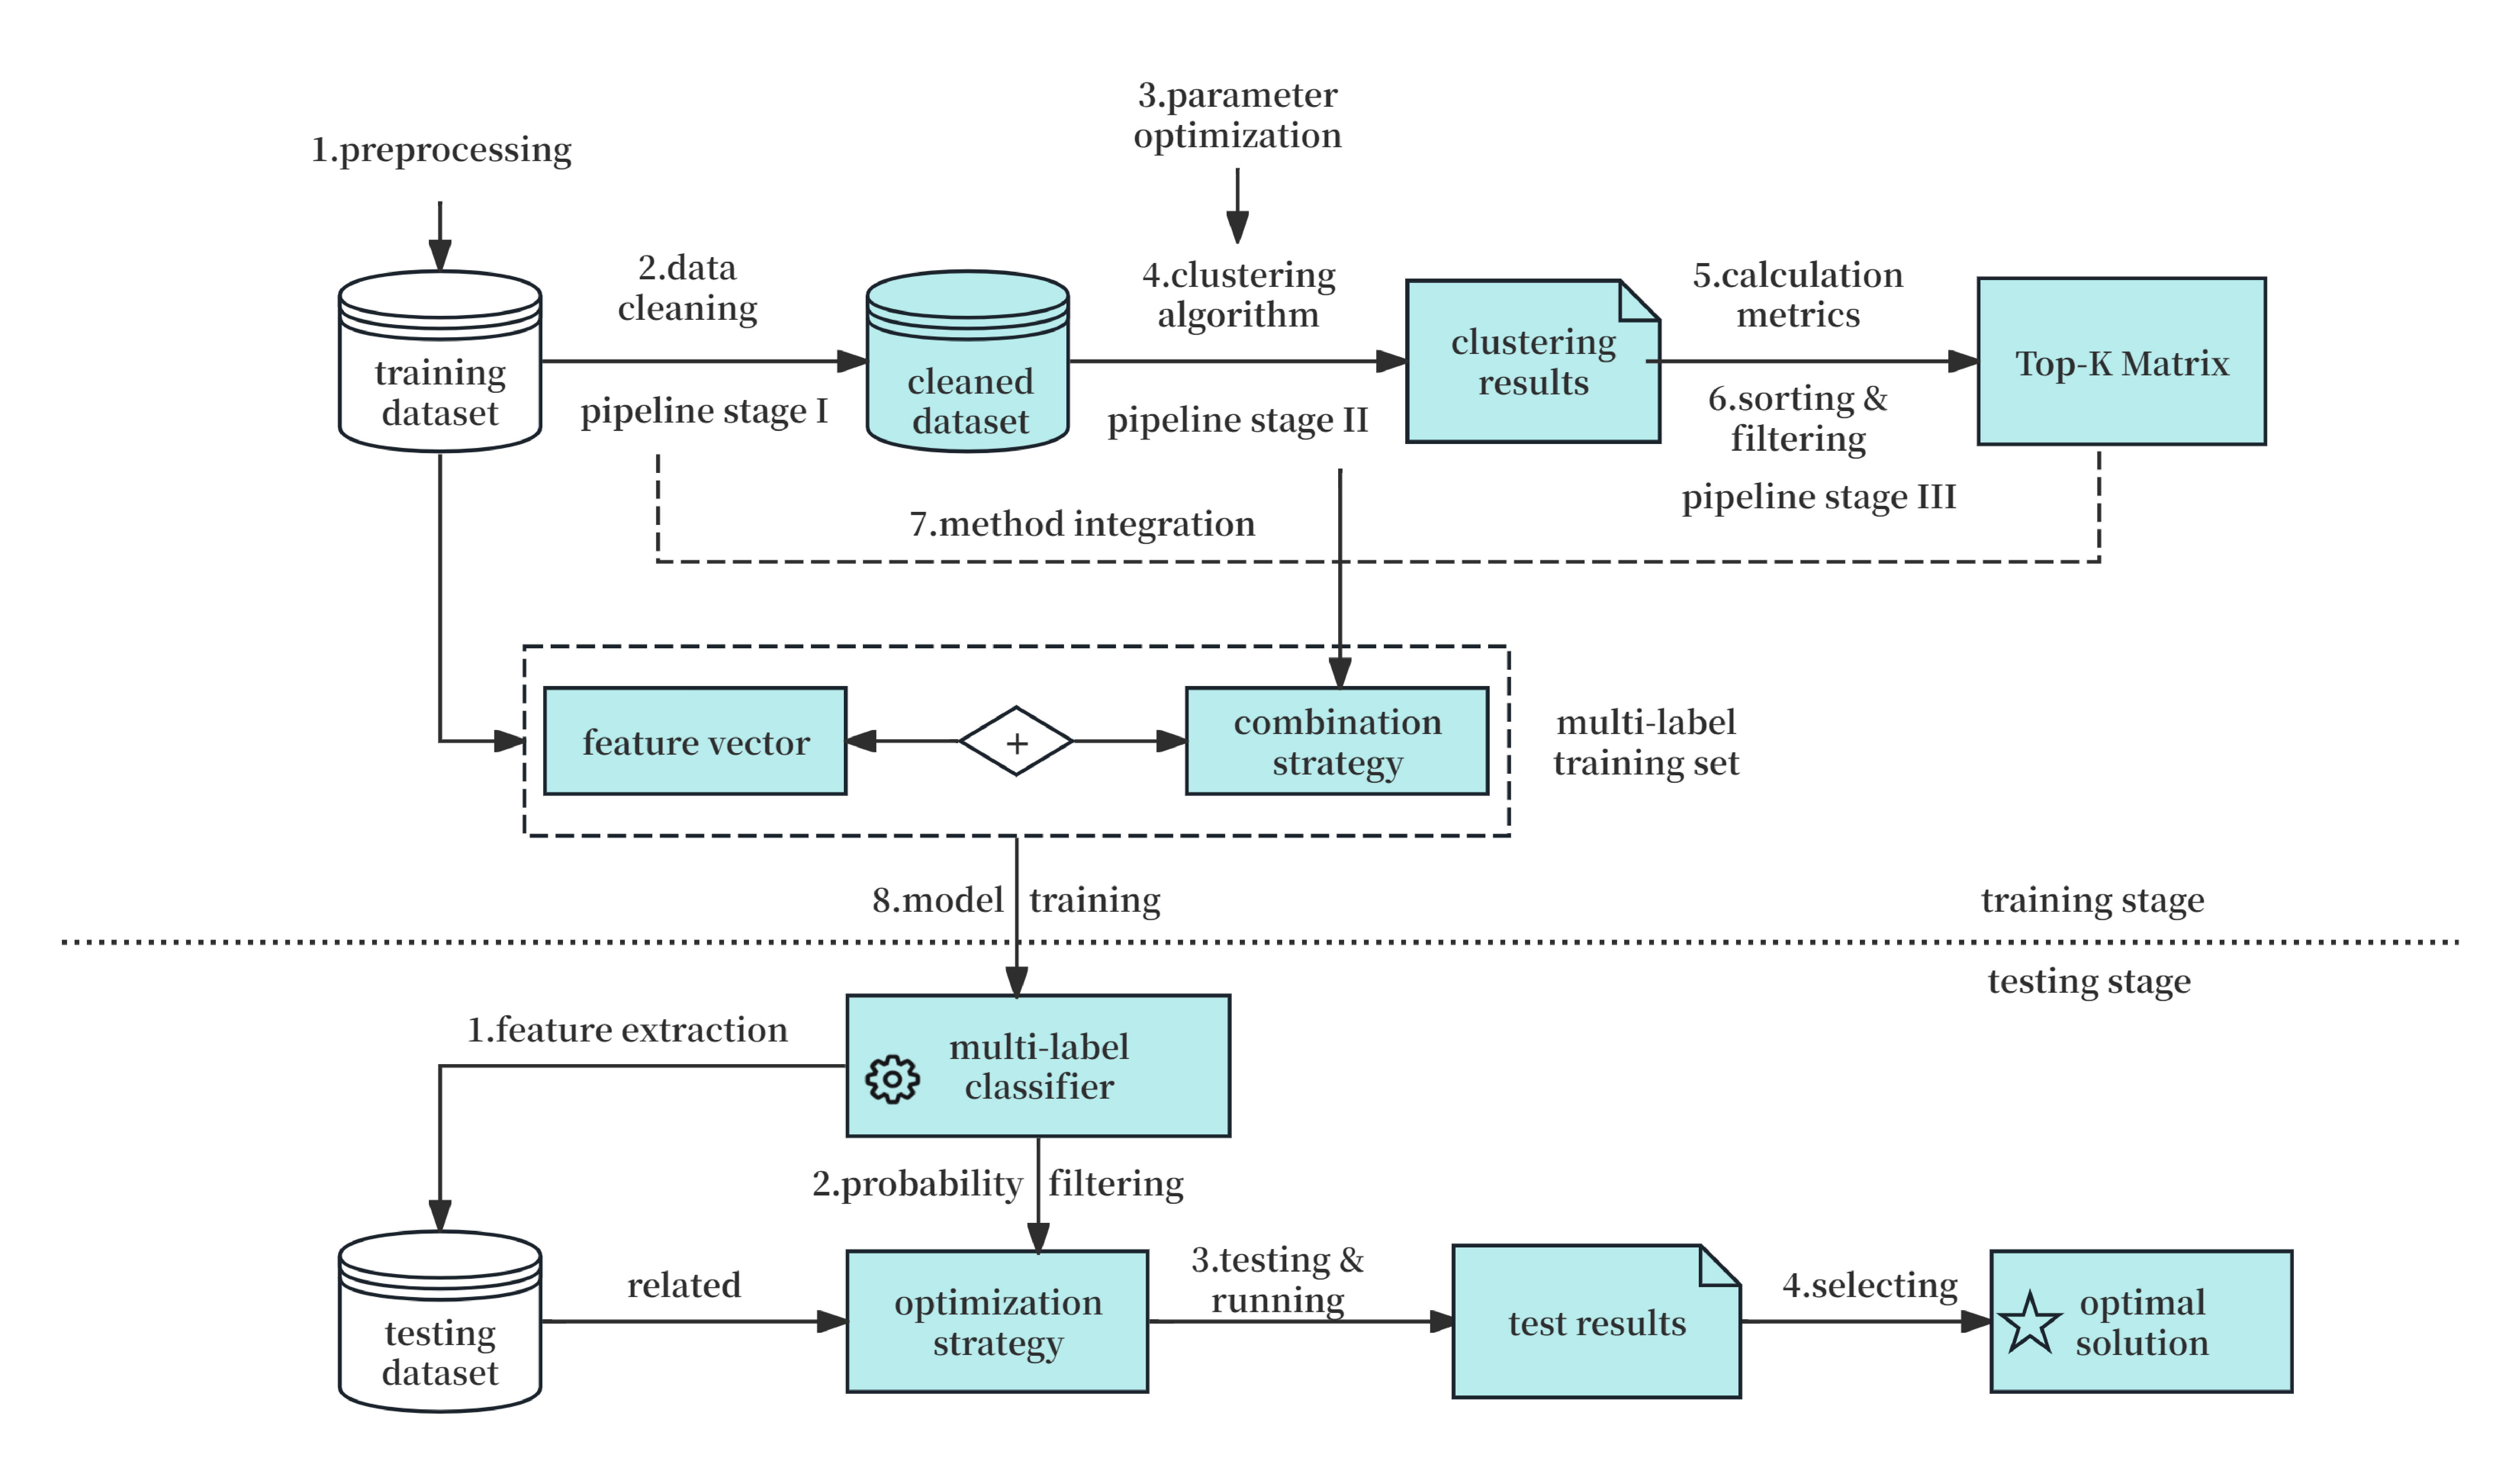
\includegraphics[width=0.9\linewidth]{figures/4graph/autocluster_workflow.pdf}
  \caption{自动化聚类优化流程示意图}
  \label{fig:autocluster-workflow}
\end{figure}

该流程主要包括\textbf{离线知识积累}(训练阶段)和\textbf{在线优化}(测试阶段)两个核心环节:
\begin{enumerate}
    \item \textbf{训练阶段(离线学习)}:基于先验数据集 $D_{\text{train}}$,计算不同数据特征与清洗-聚类策略的匹配程度,并训练多标签分类器 $\mathcal{F}$,从而建立数据特征到优选方案子空间的映射 $G(\mathbf{x}(D))$;同时收集并记录清洗准确度、聚类过程数据,以备深入机理分析。
    \item \textbf{测试阶段(在线优化)}:面对新的数据集 $D_{\text{test}}$,利用训练阶段学习到的映射 $G(\mathbf{x}(D_{\text{test}}))$,快速筛选搜索空间 $\Omega$ 中的候选策略子集 $\Omega'(D_{\text{test}})$,避免全量穷举,从而在较短时间内获取高质量的清洗-聚类方案。若需进一步探讨其内在机制,可通过与离线记录的分布及过程数据比对来解释为何某些组合在新数据上表现突出或失效。
\end{enumerate}

在接下来的小节中,我们将给出训练与测试环节的关键算法伪代码,并展示如何将多标签训练集 $\mathcal{M}$ 与在线推荐结果有机结合。

\subsubsection{训练阶段:离线知识积累}
训练阶段的目标是基于先验数据集 \(D_{\text{train}}\) 生成多标签训练集并学习多标签分类器。算法伪代码如算法~\ref{alg:train-phase} 所示。

\begin{algorithm}[t]
\small
\setlength{\tabcolsep}{6pt}
\renewcommand{\arraystretch}{1.2}
\caption{离线训练阶段:生成训练数据与训练多标签分类器}
\label{alg:train-phase}
\KwIn{
    先验数据集 $D_{\text{train}}=\{D^{(1)},\dots,D^{(N)}\}$;\\
    搜索空间 $\Omega$;\\
    Top-K 大小 $K$。
}
\KwOut{多标签分类器 $\mathcal{F}$}

\SetKwFunction{GenerateTrainingData}{GenerateTrainingData}
\SetKwFunction{TrainClassifier}{TrainClassifier}

$\mathcal{M} \leftarrow \GenerateTrainingData(D_{\text{train}}, \Omega, K)$\;
$\mathcal{F} \leftarrow \TrainClassifier(\mathcal{M})$\;
\KwRet{$\mathcal{F}$}

\bigskip

\SetKwProg{Fn}{Function}{:}{}
\Fn{\GenerateTrainingData{$D_{\text{train}}, \Omega, K$}}{
  $\mathcal{M} \leftarrow \emptyset$\;
  \For{$i \leftarrow 1$ \KwTo $|D_{\text{train}}|$}{
    \ForEach{$\omega \in \Omega$ \textbf{(或采样自 $\Omega$)}}{
      计算 $S(D^{(i)}, \omega)$\;
      记录 EDR/F1 等清洗准确度,以及算法内部过程数据(如质心迭代、核心点等)\;
    }
    选出 Top-K 策略 $\mathbf{M}^{(i)} = \{\omega_1^{(i)}, \dots, \omega_K^{(i)}\}$ 按得分降序\;
    映射为多标签集合 $\mathbf{L}^{(i)} = \{\ell_{\omega_1^{(i)}}, \dots, \ell_{\omega_K^{(i)}}\}$\;
    $\mathcal{M} \leftarrow \mathcal{M} \cup \{(\mathbf{x}(D^{(i)}), \mathbf{L}^{(i)})\}$\;
  }
  \KwRet{$\mathcal{M}$}
}

\Fn{\TrainClassifier{$\mathcal{M}$}}{
  \tcp{可根据具体多标签算法实现}
  训练多标签分类器 $\mathcal{F}$\;
  \KwRet{$\mathcal{F}$}
}
\end{algorithm}

\subsubsection{测试阶段:在线预测与最优方案搜索}
测试阶段在新数据集 \(D_{\text{test}}\) 上应用训练好的分类器,快速锁定优选子空间并搜索最优策略。伪代码如算法~\ref{alg:test-phase} 所示。

\begin{algorithm}[t]
\small
\setlength{\tabcolsep}{6pt}
\renewcommand{\arraystretch}{1.2}
\caption{测试阶段:寻找最优方案 \(\hat{\omega}\)}
\label{alg:test-phase}
\KwIn{
    测试数据集 $D_{\text{test}}$;\\
    多标签分类器 $\mathcal{F}$;\\
    搜索空间 $\Omega$;\\
    保留标签数 $r$。
}
\KwOut{最优方案 $\hat{\omega}$}

计算 $\mathbf{x}(D_{\text{test}})$\;
$\mathbf{L}' \leftarrow \{\}$\;
\ForEach{$\ell \in \mathcal{L}$}{
  $q_{\ell} \leftarrow \text{置信度}(\mathcal{F}, \mathbf{x}(D_{\text{test}}), \ell)$\;
  $\mathbf{L}' \leftarrow \mathbf{L}' \cup \{(\ell, q_{\ell})\}$\;
}
选取置信度最高的 $r$ 个标签 $\mathbf{L}'_{\mathrm{top}}$\;
映射回优选子空间 $\Omega'(D_{\text{test}})$\;
\ForEach{$\omega \in \Omega'(D_{\text{test}})$}{
    计算 $S(D_{\text{test}}, \omega)$ \tcp*{计算综合得分}
}
$\hat{\omega} \leftarrow \arg\max_{\omega \in \Omega'(D_{\text{test}})}S(D_{\text{test}}, \omega)$\;
\KwRet{$\hat{\omega}$}
\end{algorithm}

\subsection{小结}
本节系统介绍了自动化聚类方法的整体框架,从离线阶段的多标签训练与清洗准确度/过程数据记录,到在线阶段通过优选子空间快速搜索最优策略。在此基础上,我们不仅能在\textbf{大规模搜索空间}中高效获得近优清洗-聚类组合,还能借助\textbf{记录下的清洗精度与算法过程}信息,对清洗操作对聚类结果的影响机理进行更深入的剖析。下一章我们将结合具体实验展示该方法在多场景下的适用性与可解释性。


%====================  第 5 章标题  ====================
\section{实验设计与实施框架}

%==================== 5.1 数据集与噪声注入 =============
\subsection{数据集与噪声注入}
\label{sec:datasets}

\textcolor[rgb]{0.00,0.07,1.00}{本研究选择了数据清洗领域最常用且在属性类型与规模上具有互补性的四个公开数据集:\emph{beers}、\emph{flights}、\emph{hospital} 与 \emph{rayyan},它们的行列规模\((n,m)\),约束数量及列类型分布见表 \ref{tab:dataset_overview}。为了在可复现的条件下系统评估“清洗–聚类”管线的稳健性,我们注入两类最基础且工业场景最常见的错误:缺失值 (Missing) 与异常值 (Anomaly)。具体做法是对每个数据集的干净基线版本,在除主键列外的所有单元格上独立采样\((\text{AnomalyRate},
\text{MissingRate})\in\{0,5,10,15\}\%\times\{0,5,10,15\}\%\),
共构造 \(4\times4-1=15\) 份含错文件(剔除 \(0\%–0\%\) 组合),并以表 \ref{tab:error_def} 所列规则生成脏值。注入后得到的观测总错误率定义为\(r_{\text{tot}}=r_{\text{anom}}+r_{\text{miss}}\),
其区间分布将作为后续实验分档与特征提取的依据。}
\begin{table}[htbp]
  \centering\small
  \setlength{\tabcolsep}{6pt}
  \renewcommand{\arraystretch}{1.2}
  \caption{四个数据集的规模、列类型统计及约束数量(数值、文本、混合)}
  \begin{tabular}{lcccccc}
    \toprule
    \textbf{Dataset} & $\boldsymbol{n}$ & $\boldsymbol{m}$ & \textbf{数值列} & \textbf{文本列} & \textbf{混合列} & \textbf{约束数量}\\
    \midrule
    beers    & 2\,410 & 11 & 6 & 4 & 1 & 5 \\
    flights  & 2\,376 & 7  & 1 & 1 & 4 & 6 \\
    hospital & 1\,000 & 20 & 5 & 11 & 4 & 15 \\
    rayyan   & 1\,000 & 12 & 5 & 5 & 2 & 10 \\
    \bottomrule
  \end{tabular}
  %\end{adjustbox}
  \label{tab:dataset_overview}
\end{table}

\begin{table}[htbp]
  \centering\small
  \setlength{\tabcolsep}{6pt}
  \renewcommand{\arraystretch}{1.2}
  \caption{错误类型定义、注入规则与对应错误率}
  \begin{tabular}{llllll} % ← 列数由 5 ➜ 6
    \toprule
    \textbf{错误类型定义} & \textbf{原值(干净)} & \textbf{脏值} &
    \textbf{错误率定义} & \textbf{规则 \& 生成方法} & \textbf{与其他错误重叠}\\
    \midrule
    异常值 (A) &
      非空 &
      非空且 $\neq$ 原值 &
      $\displaystyle r_{\text{anom}}
        =\frac{|A|}{N_{\text{non--NaN}}}$ &
      \begin{tabular}[c]{@{}l@{}}
        \textbf{数值列}: $x \leftarrow x \times U(3,6)$\\[-2pt]
        \textbf{文本列}: 随机在字符串中\\[-2pt]
        \hspace*{1em}插入 $1$--$2$ 个符号片段\\[-2pt]
      \end{tabular} &
      不与缺失重叠 \\
    \addlinespace[2pt]
    缺失值 (M) &
      非空 &
      空值 (\texttt{NaN}) &
      $\displaystyle r_{\text{miss}}
        =\frac{|M|}{N_{\text{non--NaN}}}$ &
      从剩余非空候选中随机采样 &
      不与异常值重叠 \\
    \addlinespace[2pt]
    非错误 &
      非空值 &
      非空且 = 原值 &
      -- &
      保持原本为非空的数据不变 &
      -- \\
    \addlinespace[2pt]
           &
      空值 &
      空值 &
      -- &
      保持原本为空的数据不变 &
      -- \\
    \bottomrule
  \end{tabular}
  \label{tab:error_def}
\end{table}


\subsection{数据清洗模块:算法库与评价指标}
\label{sec:algo_prep}

\subsubsection{算法目录}
\label{sec:algo_cat}

\textcolor[rgb]{0.00,0.07,1.00}{为便于后续实验复现与横向比较,表 \ref{tab:clean_algo_overview} 初步汇总了本研究选取的 9 种清洗方法的关键信息,覆盖统计、规则与机器学习三大范式。}

\begin{table}[t]
\centering\small
\renewcommand{\arraystretch}{1.2}
\setlength{\tabcolsep}{6pt}
%\begin{adjustbox}{width=\linewidth}
\caption{本实验选取的 9 种数据清洗方法总览}
\begin{tabular}{@{}lcccc@{}}
\toprule
\textbf{算法} & \textbf{针对错误类型} & \textbf{必需配置} &
\textbf{模型范式} & \textbf{清洗目标} \\
\midrule
Mode Impute & MV, FI & — &
统计填补 & \textit{Repair} \\

Raha-Baran & MV, FI, Rule viol. & 无显式约束 &
端到端 ML & \textit{Detect + Repair} \\

HoloClean & MV, FI, Dup, Rule viol. &
FD/CF + 外部知识 &
概率图模型 & \textit{Detect + Repair} \\

BigDansing & Schema viol., Typos &
检测规则 & 规则驱动 & \textit{Detect} \\

BoostClean & Label/Attr Noise &
下游模型 (监督) &
Boosting Ensemble & Task–Aware Repair \\

Horizon & MV, Outlier &
时序窗口宽度 &
时序/统计混合 & \textit{Repair} \\

Scared & MV, FI, Outlier &
半监督标注预算 &
主动学习模型 & \textit{Detect + Repair} \\

Unified & MV, Rule viol., Dup &
统一约束文件 &
多策略融合 & \textit{Detect + Repair} \\

GroundTruth & — & — &
理想基线 & \textit{Upper Bound} \\
\bottomrule
\multicolumn{5}{l}{\footnotesize
MV: Missing Value;FI: Format Inconsistency;Dup: Duplicate;Rule~viol.: 约束违规。}
\end{tabular}
%\end{adjustbox}
\label{tab:clean_algo_overview}
\end{table}

\vspace{-1em}
\subsubsection{单元格级评估指标}\label{sec:metrics}
\textcolor[rgb]{0.00,0.07,1.00}{本小节旨在说明\textbf{如何对9种清洗算法的单元格级表现进行系统量化},
从而为第 6 章的结果比较和机理分析奠定统一度量基础。
与前小节的算法库(表 \ref{tab:clean_algo_overview})相对应,
我们首先给出基于 \emph{Before/After} 状态的 $2\times2$ 混淆矩阵,
随后从该矩阵派生 Precision、Recall、F1 及
\emph{Error‑Drop Rate (EDR)} 等公式。所有指标均对
\{\textit{Anomaly},\,\textit{Missing}\} 两类错误求和,
具体符号定义见表 \ref{tab:cell-metrics-def}。}

\begin{table}[ht]
\centering\small
\setlength{\tabcolsep}{6pt}
\renewcommand{\arraystretch}{1.25}
\caption{单元格级混淆矩阵及派生指标 Precision, Recall, F1, EDR}
\begin{tabular}{c|cc}
\toprule
 & \multicolumn{2}{c}{\textbf{修改后}}\\\cline{2-3}
\textbf{修改前} & 正确 (R) & 错误 (W)\\\hline
错误 (W) & TP & FN\\
正确 (R) & FP & TN\\
\bottomrule
\end{tabular}

\vspace{0.6em}
\begin{tabular}{@{}lp{9.5cm}@{}}
\toprule
\textbf{符号} & \textbf{定义/含义} \\
\midrule
$TP$ & 错误单元格被正确修复\\
$FP$ & 正确单元格被误改坏\\
$FN$ & 错误单元格未被修复\\
$TN$ & 正确单元格保持正确\\
\midrule
$\displaystyle\text{Precision}=\frac{TP}{TP+FP}$ &
改动中有多少是真正修复 \\[4pt]
$\displaystyle\text{Recall}=\frac{TP}{TP+FN}$ &
原有错误中有多少被修复 \\[4pt]
$\displaystyle\text{\(F_1\)}=\frac{2\,\text{Prec}\,\text{Rec}}{\text{Prec}+\text{Rec}}$ &
综合精确率与召回率 \\[6pt]
$\displaystyle\text{EDR}=\frac{TP-FP}{TP+FN}$ &
\emph{净}改进率:单位原始错误的净收益 \\
\bottomrule
\end{tabular}
\label{tab:cell-metrics-def}
\end{table}

\subsection{聚类算法及超参数}\label{sec:clu_algo}

\textcolor[rgb]{0.00,0.07,1.00}{为支撑后续因果验证,本节统一说明6类定制化聚类脚本在初始化策略、超参搜索维度、过程级指标(含期望方向)及复杂度变化四个维度上的设定,相关符号与缩写沿用前文。表~\ref{tab:algo_full} 汇总了全部信息,所有超参数均通过 \texttt{Optuna} 网格枚举,并在第\,6\,章结合过程曲线进行机理解析。}

\begin{table}[t]
  \centering\small
  \setlength{\tabcolsep}{6pt}
  \renewcommand{\arraystretch}{1.07}
  \caption{6类聚类脚本的主要概览(\(\downarrow/\uparrow\) 表示指标的期望改善方向)。}
  \begin{tabular}{@{}lcccc@{}}
    \toprule
    \textbf{算法脚本} &
    \textbf{初始化/采样} &
    \textbf{调优维度} &
    \makecell[c]{\textbf{过程指标}\\(期望方向)} &
    \makecell[c]{\textbf{复杂度}\\(相对变化)} \\ 
    \midrule
    \multicolumn{5}{@{}l}{\textit{质心型}}\\
    K-Means\textsubscript{base} &
      k-means++ &
      $k$ &
      \(\Delta n_{\text{iter}}\!\downarrow,\;\text{GeoDecay}\!\downarrow,\;\text{AUC}_\Delta\!\downarrow\) &
      \(\mathcal{O}(nkT)\) \\[2pt]
    K-Means\textsubscript{PPS}\cite{10.5555/3016100.3016103} &
      K-MC$^{2}$ &
      $k$ &
      同上 &
      \(\mathcal{O}(n)\) 初始化$\;\!\downarrow$ \\[2pt]
    K-Means\textsubscript{NF}\cite{10.1109/TKDE.2022.3155450} &
      随机标签$\!\to\!F$ &
      $k$ &
      同上 &
      Gram 计算$\;\uparrow$ \\[4pt]
    \multicolumn{5}{@{}l}{\textit{模型型}}\\
    GMM--EM\,(tracking) &
      k-means++ &
      $k$(Kneedle) &
      \(\Delta n_{\text{iter}}\!\downarrow,\;\text{AUC}_{\text{LL}}\!\downarrow\) &
      warm--start 循环$\;\uparrow$ \\[4pt]
    \multicolumn{5}{@{}l}{\textit{密度型}}\\
    DBSCAN\,(noise--aware) &
      — &
      \(\varepsilon,\; \text{minPts}\) &
      \(\Delta n_{\text{core}}\!\uparrow,\;\Delta\rho_{\text{noise}}\!\downarrow,\;\Delta W_{\text{cdf}}\!\downarrow\) &
      \(\mathcal{O}(n\log n)\) \\[4pt]
    \multicolumn{5}{@{}l}{\textit{层次型}}\\
    HC\,(merge--tree) &
      — &
      $k$、linkage、metric &
      \(\Delta n_{\text{merge}}\!\downarrow,\;\Delta h_{\max}\!\downarrow,\;\Delta R_{\text{intra/inter}}\!\downarrow\) &
      \(\mathcal{O}(n^{2})\) \\
    \bottomrule
  \end{tabular}
  \label{tab:algo_full}
\end{table}

\textcolor[rgb]{0.00,0.07,1.00}{为使后续大规模对比实验中的评价既无监督又可跨数据集或算法直接比较,
我们首先将
\[
\text{Sil}\in[-1,1],\qquad 
\text{DB}\in(0,\infty)
\]
统一映射到同向同尺度区间
\[
S=\frac{\text{Sil}+1}{2}\in[0,1],\qquad 
D=\frac{1}{1+\text{DB}}\in(0,1],
\]
并采用\emph{加权调和平均}
\[
\text{CI}_{\mathrm{harm}}(\alpha)=
\frac{1}{\dfrac{\alpha}{S}+\dfrac{1-\alpha}{D}},\qquad 
\alpha\in[0,1]
\]
作为总评价指标,令 $\alpha$ 决定两项度量的相对权重。}

\textcolor[rgb]{0.00,0.07,1.00}{为确定 $\alpha$ 的最优取值,我们设计了一个权重网格预实验;
Algorithm \ref{alg:grid} 给出了完全自动化的流程:外层遍历
$\alpha$ 网格,内层对所有\emph{数据集--算法}组合调用
\textsc{Optuna} 最大化 $\text{CI}_{\mathrm{harm}}(\alpha)$,
随后统计每个 $\alpha$ 的
\emph{最大方差} $v_{\max}(\alpha)$ 与 \emph{中位均值} $m_{\mathrm{avg}}(\alpha)$,
并借助 \texttt{kneed.KneeLocator} 函数在
$\bigl\{(\alpha,\,m_{\mathrm{avg}}(\alpha))\bigr\}$ 轨迹上寻找经典肘部
$\alpha_{\text{elbow}}$。}

\begin{algorithm}[t]
\small
\setlength{\tabcolsep}{6pt}
\renewcommand{\arraystretch}{1.2}
\caption{\textcolor[rgb]{0.00,0.07,1.00}{预实验阶段:权重网格搜索与肘部检测}}
\label{alg:grid}
\KwIn{
  数据集集合 $\mathcal{D}$(大小 $|\mathcal{D}|$);
  算法集合 $\mathcal{A}$(大小 $|\mathcal{A}|$);\\
  $\alpha$ 网格 $\mathcal{G}=\{\alpha_1,\dots,\alpha_{n_\alpha}\}$;
  \textsc{Optuna} trial 数 $N$
}
\KwOut{
  结果表 $\bigl[\alpha_i,\,v_{\max}(\alpha_i),\,m_{\mathrm{avg}}(\alpha_i)\bigr]_{i=1}^{n_\alpha}$;
  肘部权重 $\alpha_{\text{elbow}}$
}

\ForEach{$\alpha_i\in\mathcal{G}$}{
  \ForEach{$(d,a)\in\mathcal{D}\times\mathcal{A}$ \textbf{并行}}{
    在算法 $a$ 的超参数空间用 \textsc{Optuna} 进行 $N$ 次贝叶斯优化,\\
    得到最优得分 $s_{d,a}^{(\alpha_i)}$\;
  }
  计算数据集内方差
  $\text{Var}_d(\alpha_i)=
  \operatorname{Var}\{s_{d,a}^{(\alpha_i)}\}_{a\in\mathcal{A}}$\;
  以及中位数
  $\widetilde m_d(\alpha_i)=
  \operatorname{median}\{s_{d,a}^{(\alpha_i)}\}_{a\in\mathcal{A}}$\;
  \[
  v_{\max}(\alpha_i)=\max_{d}\text{Var}_d(\alpha_i),\qquad
  m_{\mathrm{avg}}(\alpha_i)=
  \frac{1}{|\mathcal{D}|}\sum_{d}\widetilde m_d(\alpha_i)
  \]
}
用 \texttt{kneed.KneeLocator}$\bigl(\{\alpha_i\},\{m_{\mathrm{avg}}(\alpha_i)\}\bigr)$\\
检测肘部并返回 $\alpha_{\text{elbow}}$\;
\KwRet 结果表及 $\alpha_{\text{elbow}}$
\end{algorithm}

\textcolor[rgb]{0.00,0.07,1.00}{在实际预实验中,我们取 $|\mathcal{D}|=4$、$|\mathcal{A}|=6$,
$\mathcal{G}$ 设为 $20$ 等分的线性网格,内层
\textsc{Optuna} trial 数 $N=20$。
统计得到的
$m_{\mathrm{avg}}(\alpha)$ 随 $\alpha$ 单调上升,
而 $v_{\max}(\alpha)$ 单调下降;
对 $m_{\mathrm{avg}}$ 曲线作二阶差分并再次调用
\texttt{kneed},肘部出现在
\[
\boxed{\alpha_{\text{elbow}}\approx0.47}.
\]
图~\ref{fig:alpha-vs-median} 与图~\ref{fig:alpha-vs-var}
分别给出了 $\alpha$ 对应的 $m_{\mathrm{avg}}$ 与 $v_{\max}$ 折线以及二阶导曲线。
后续正式实验固定
$\alpha^\star=\alpha_{\text{elbow}}$
以兼顾较高的平均得分与显著降低的跨算法方差。}

\begin{figure}[t]
  \centering
  \begin{subfigure}{0.49\linewidth}
    \centering
    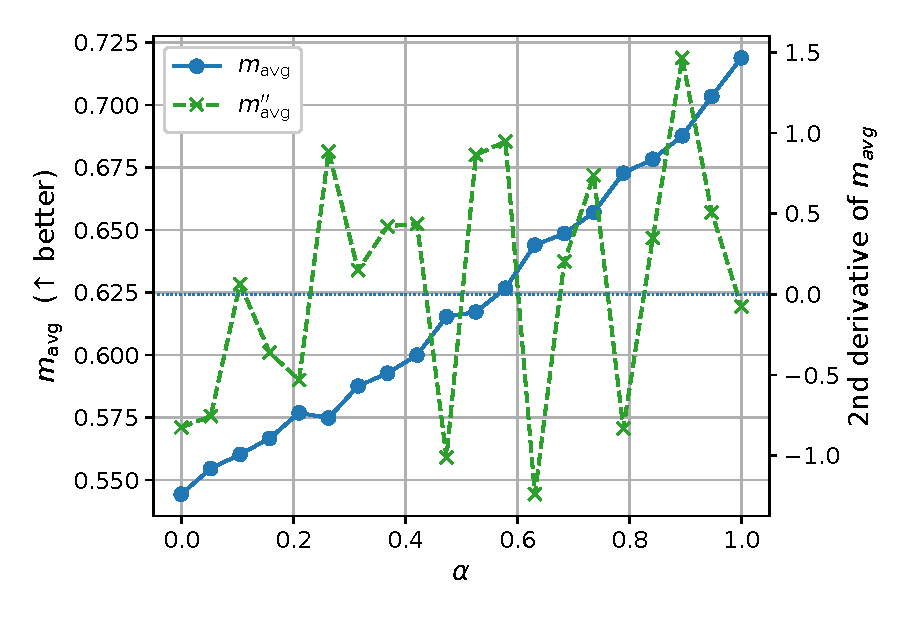
\includegraphics[width=\linewidth]{figures/4graph/alpha_vs_median.eps}
    \caption{$\alpha$–$m_{\mathrm{avg}}$ 折线及二阶导}
    \label{fig:alpha-vs-median}
  \end{subfigure}\hfill
  \begin{subfigure}{0.49\linewidth}
    \centering
    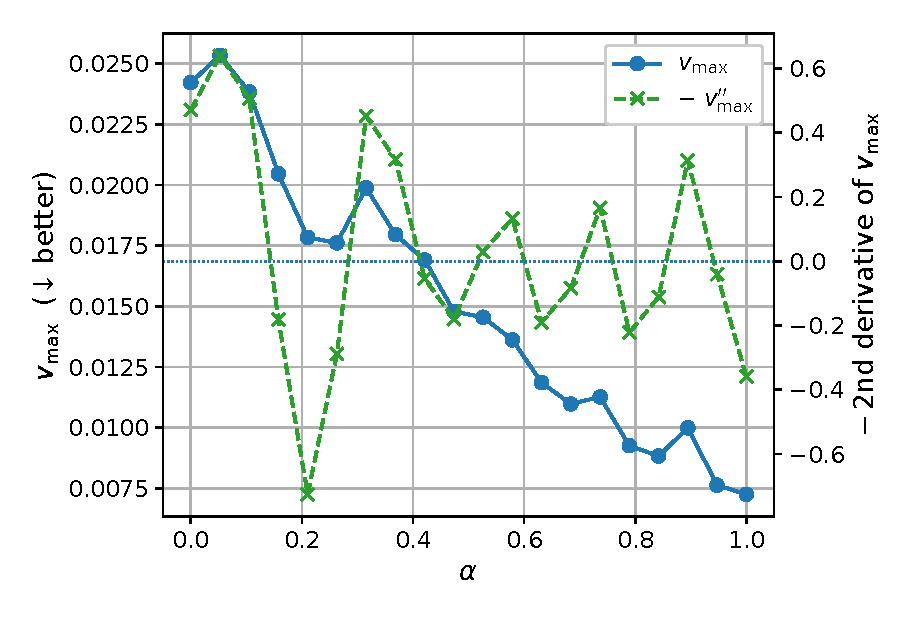
\includegraphics[width=\linewidth]{figures/4graph/alpha_vs_variance.eps}
    \caption{$\alpha$–$v_{\max}$ 折线及二阶导(取相反数)}
    \label{fig:alpha-vs-var}
  \end{subfigure}
  \caption{权重网格预实验:平均得分与最大方差随 $\alpha$ 变化曲线}
\end{figure}

%--------------------------------------------------
\subsection{\textcolor[rgb]{0.00,0.07,1.00}{实验设计流程}}\label{sec:exp_pipeline}

为验证前文提出的“清洗–聚类协同优化”假设,本节依托图~\ref{fig:exp_flow} 所示的统一流水线组织全部实验。该流水线由离线测评、元学习训练与在线评估三环节构成:首先在完全可控的环境中获取可复现的实验现象,随后循迹揭示影响机理并抽取可迁移规律,最终将模型化知识应用到真实业务场景。

离线测评阶段以4张公开数据表为基准,在 \(\langle r_{\text{miss}},r_{\text{anom}}\rangle\) 网格上注入多档噪声,并分别施加9种清洗策略与6类聚类脚本。流水线自左而右依次执行:错误注入与特征提取,预聚类标准搜索,清洗批处理,聚类及过程跟踪,评价指标计算与分档,最终得到实验原始记录,其中包括修复标签、过程日志、终态得分与最优超参。

基于上述记录,我们首先对不同清洗–聚类管线的性能指标做定性比较,初步判断清洗量与聚类质量的相关性以及各算法族对噪声的敏感度。随后进入定量剖析阶段,旨在明确回答“数据清洗究竟在何时、以何种程度对聚类起作用”,并从以下三个互补视角展开论证:

\emph{(i)过程动力学视角:} 以迭代轮次 \(\Delta n_{\text{iter}}\),几何衰减率 \(\text{GeoDecay}\) 与核心点计数 \(\Delta n_{\text{core}}\) 等过程指标为观测对象,比较清洗前后的相对改变量,刻画清洗对收敛速度、噪声判定稳定性及层次树紧凑度的影响时机与幅度,回答清洗是否实质改变聚类算法运行的内部过程。

\emph{(ii)结果映射视角:} 在单元格级修复准确度(EDR、Precision、Recall、\(F_1\))与聚类评价指标(Silhouette、Davies–Bouldin、Combined) 之间建立多项式分段回归分析模型,识别清洗量的线性、阈值或饱和区段,以回答清洗准确度能否、以及在何种程度上转化为聚类指标收益。

\emph{(iii)超参数漂移视角:} 追踪 Optuna 的超参寻优轨迹,比较清洗前后最优参数 \(k^\star\)、\(\varepsilon^\star\) 及协方差结构的系统性漂移,并以二维 KDE 描绘差分分布 \(p(\Delta k,\Delta\varepsilon)\),回答数据质量与清洗策略的变化对聚类的最优超参数造成何种“漂移”,并如何利用这种漂移动态调整 AutoML 的搜索空间。\\
三重视角层层递进地构成“行为 $\rightarrow$ 结果 $\rightarrow$ 超参”的因果链:\emph{过程动力学} 揭示清洗对聚类内部机制的即时效应,\emph{结果映射} 量化该效应在评价层面的收益转化,而 \emph{超参数漂移} 则捕捉收益最大化所伴随的搜索空间重塑。三类证据均在同一数据基线上获取,可相互校验并消解单点偏差。

元学习训练阶段,我们将上述“数据特征—策略选择—评分收益”的三元规律转化为可调用的知识,把不同数据集的特征及多种历史搜索管线抽象为一组特征向量(称为配置),然后在离线阶段学习该配置到综合评分的映射,从而训练并构建多标签预测器 $\varPhi$ 。随后在搜索时利用该预测器逐层扩展管线树并在置信不足时裁剪,得到搜索子空间 $\Omega' \subset \Omega$。 

在线评估阶段,我们对新应用场景的数据集 $D^\ast$ 进行特征提取,并将其输入预测器 $\varPhi$ 得到优选子空间 $\Omega'_\ast$,随后在 $\Omega'_\ast$ 内进行局部搜索得到估测的最优组合 $\hat{\pi}$。将该结果与无先验的全空间搜索基线进行对照,记录并比较二者在搜索时间、CPU 利用率与聚类质量上的差异。 

综上,统一流水线以一次离线批量运行形成“现象观测—机理剖析—规律抽取—模型训练”的四层闭环,并生成可直接驱动搜索裁剪的预测器 \(\varPhi\) 以供在线验证。下一章将基于这些原始数据与模型结果,系统阐释清洗—聚类协同效应的实证发现及规律,并给出对 AutoML 动态优化策略的定量评估。

\begin{figure}[t]
  \centering
  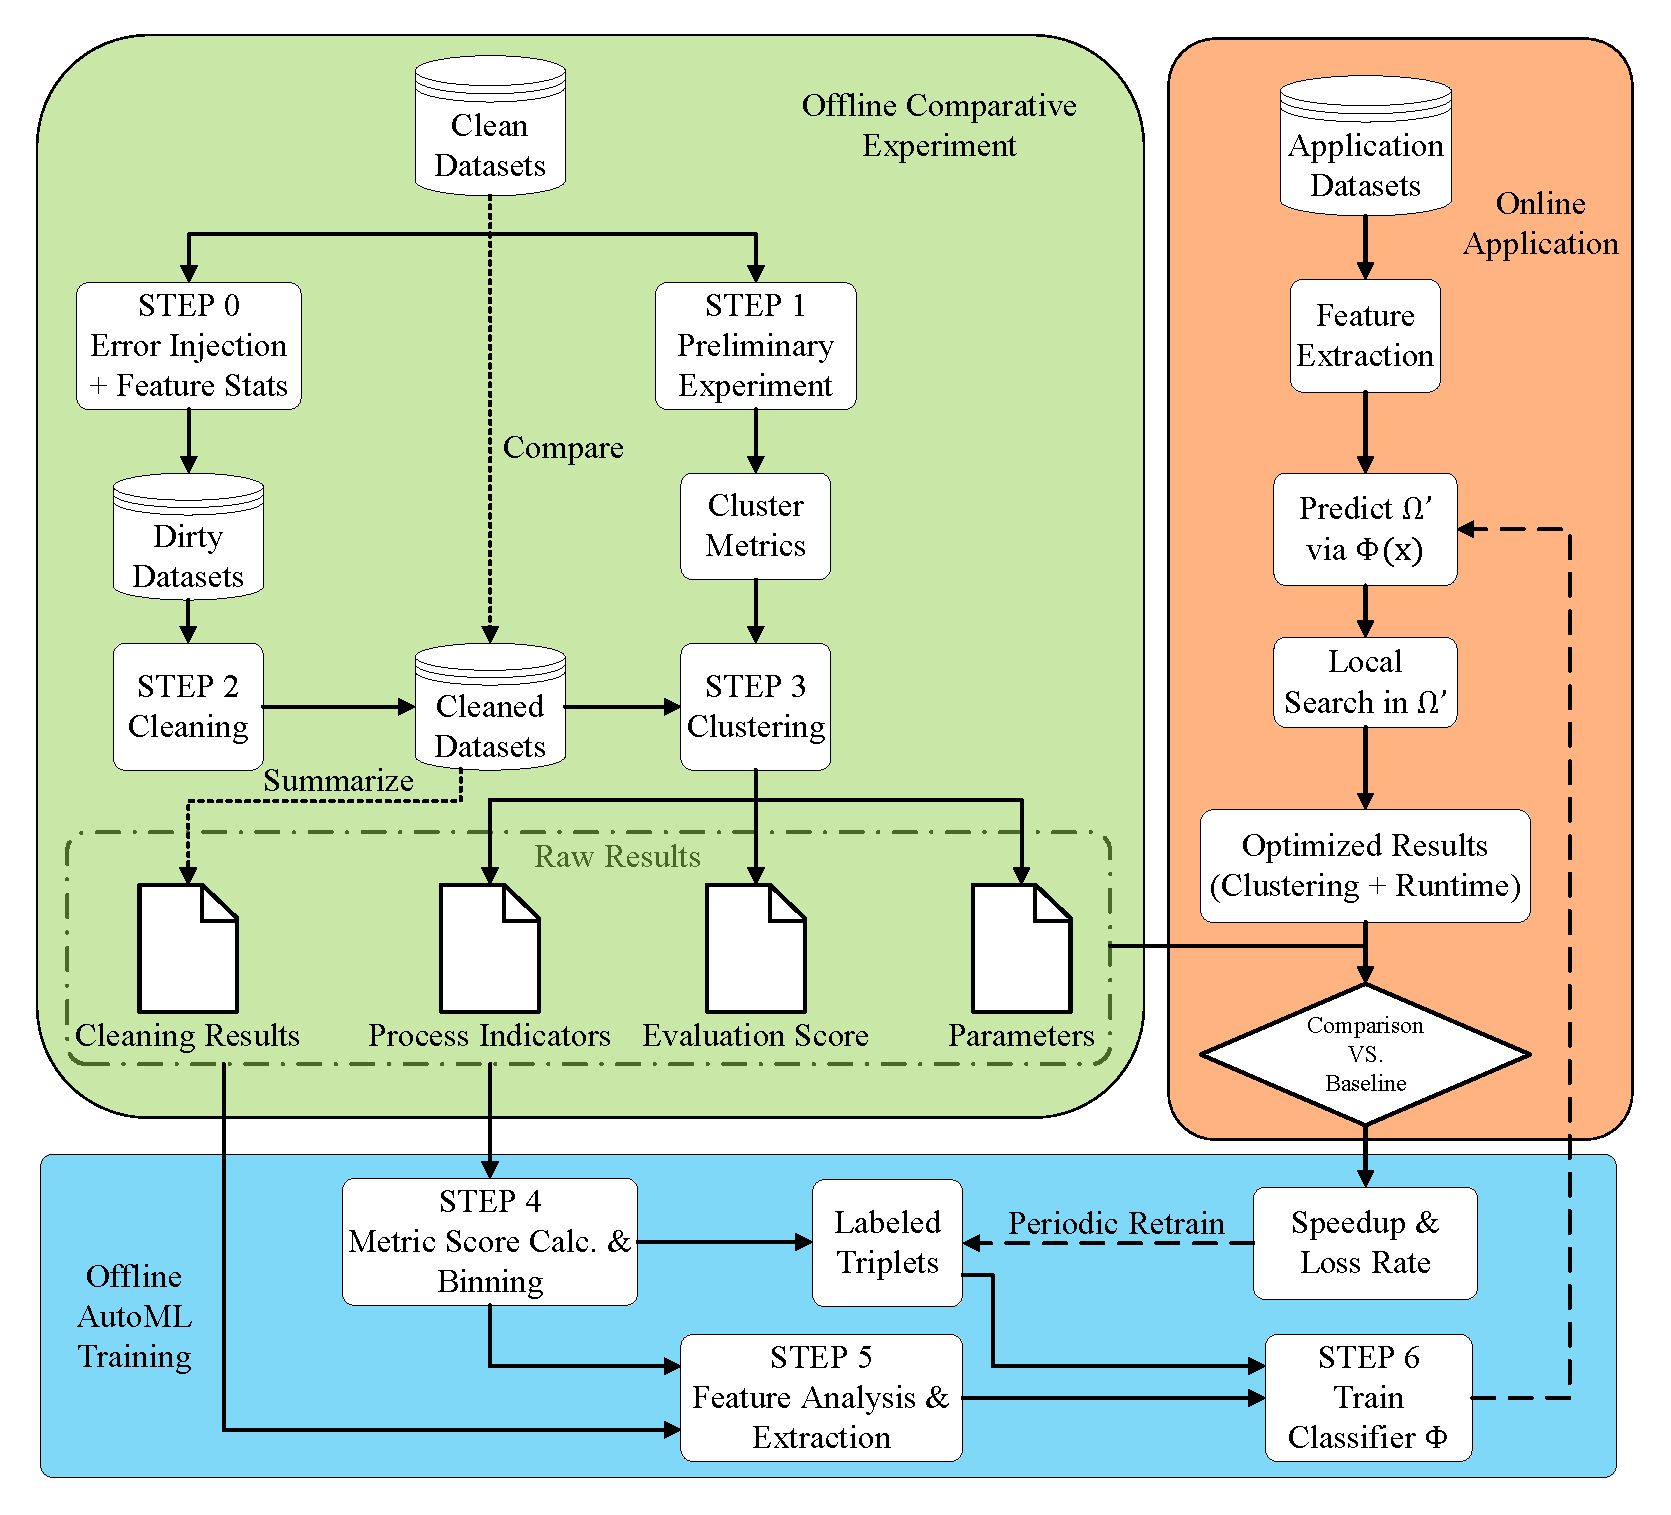
\includegraphics[width=0.95\linewidth]{figures/4graph/flowchart1.pdf}
  \caption{本研究中批量实验的流水线示意图}
  \label{fig:exp_flow}
\end{figure}

\section{机理分析与 AutoML 优化}
\label{sec:chapter6}
%====================================================================

\vspace{-0.3em}
\noindent

根据第\,\ref{sec:exp_pipeline}节的实验设计,我们利用统一流水线依次完成了\textit{错误注入 $\rightarrow$ 清洗批处理 $\rightarrow$ 聚类跟踪 $\rightarrow$ 指标分档} 的全链评测,获得了四组互补的原始实验结果:\emph{单元格级检测指标}、\emph{聚类过程日志}、\emph{综合质量得分} 以及 \emph{最优超参轨迹}。本章在此基础上依次从以下四个角度探讨数据清洗对下游聚类的影响——清洗准确度(Q\textsubscript{1})、过程干预(Q\textsubscript{2})、收益映射(Q\textsubscript{3}) 与超参漂移(Q\textsubscript{4}),并据此提炼可落地的 AutoML 动态优化策略。

%--------------------------------------------------
\subsection{\textcolor[rgb]{0.00,0.07,1.00}{清洗准确度对聚类质量的作用机制}}
\label{sec:exp_results}
%------------------------------------------------------------------

本小节聚焦\emph{全局对照} 结果,利用原始数据中对清洗-聚类的得分评估以及错误类型敏感性的记录,从“相对收益、波动风险、极值分布”三个不同的角度分别绘制了\emph{热力图}、\emph{均值–方差散点图} 与\emph{Top‑10误差条形图} (见 Fig.\,\ref{fig:score_eval_all})。我们分析了不同清洗指标对聚类的影响,阐明了清洗覆盖度∕精度在不同噪声强度下的权衡,并指出多种组合策略在不同场景下的稳健优势及失效条件。我们将有助于AutoML优化的跨数据集发现归纳至表\ref{tab:global_findings_refined1} 。

% 需在导言区 \usepackage{tabularx}
\begin{table}[t]
  \centering\small
  \setlength{\tabcolsep}{6pt}
  \renewcommand{\arraystretch}{1.25}
  \caption{§6.1的6条核心发现($\checkmark$ 表示结果与通常的直觉相悖)}
  \begin{tabularx}{\textwidth}{@{\extracolsep{\fill}}c X X X c@{}}
    \toprule
    \# & \textbf{量化发现} & \textbf{数据支撑} & \textbf{结论意义} & \textbf{是否反直觉} \\
    \midrule
    1 &
      \emph{EDR比\(F_1\)更能解释清洗对聚类收益的作用} &
      Fig.\,5‑3‑1 散点;§6.1.1 & 
      将EDR设为清洗‑聚类协同优化的首要目标 & $\checkmark$ \\
    2 &
      “众数+HC” 默认最优,且最佳错误率阈值随任务从5\%→20\%漂移 &
      Fig.\,5‑3‑1/5‑3‑2; §6.1.1–6.1.2 &
      提供一条通用默认轨迹,同时指导 EDR 上限需任务自适应 &  \\ 
    3 &
      修复优先级:缺失>异常,且异常占比\(\geq10\%\) 时收益反转 &
      Fig.\,5‑3‑2 热力图;§6.1.2 &
      建议流水线按从Missing再到Anomaly分阶段清洗 & $\checkmark$ \\ 
    4 &
      HC在超高噪声 (\(\ge30\%\)) 段仍保持前二平均秩 &
      Fig.\,5‑3‑2 清洗-聚类曲线;§6.1.2 &
      为极端脏数据提供稳健兜底聚类策略 &  \\ 
    5 &
      文本语料冗余场景下 “众数+DBSCAN” 反超HC &
      Fig.\,5‑3‑1 Top‑10;§6.1.3 &
      高密度文本应切换到DBSCAN并放宽\(\varepsilon\) & $\checkmark$ \\ 
    6 &
      Ground‑Truth清洗并非聚类最优基线,过度修复压平梯度 &
      Fig.\,5‑3‑2 热力图;§6.1.2 &
      不应以单元格\(F_1\)为唯一清洗目标 & $\checkmark$ \\ 
    \bottomrule
  \end{tabularx}
  \label{tab:global_findings_refined1}
\end{table}


%─────────────────────────────────────────────
\subsubsection{全局对照:收益–风险权衡}
\label{subsec:global_contrast}

\medskip
\noindent%
\textbf{稳健默认组合.}\;
在四个数据集的 Top‑10 榜单中,\texttt{mode+HC} 与 \texttt{GT+HC}
分别17次与13次位列首位——两者在 Friedman 检验
\((\chi^{2}{=}1671.4,\,p{<}10^{-16})\) 下无显著差异,
并共同将均值–方差散点控制在
\(\overline{S}_{\%\mathrm{GT}}>110\%,\,\sigma^{2}_{S}<1\) 的低风险高收益象限。
这一现象说明“轻度众数填补 + 层次聚类”可以作为默认分支写入
AutoML 策略库,前提是后续调参过程中监控
\(\Delta\mathrm{Sil}\) 与 \(\Delta\mathrm{DBI}\) 的同向性以防梯度被压平。

\medskip
\noindent%
\textbf{文本场景的密度法反超.}\;
在以文本向量为主的\textit{rayyan}数据集上,
\texttt{mode+DBSCAN} 的综合得分比 HC 组合高出约0.4,
且误差条几乎完全落在 HC 置信区间之外。
高语义冗余文本在向量空间形成致密块,
使 DBSCAN 能避免 HC 的簇碎片化。
因此在相似语料驱动的场景下,
AutoML 应将密度法提至首选并适当放宽\(\varepsilon\) 搜索上界。

\medskip
\noindent%
\textbf{EDR 的决定性优先于\(F_1\).}\;
根据表\ref{tab:q1-acc-all} 中的数据计算得到:净修复量指标 \textit{EDR}在Missing 单元格的全局平均值为 0.41,Anomaly中为 0.17。对 28 组“数据集×错误率”样本的相关性分析表明,\textit{EDR} 与下游 \textit{Combined Score} 的 Pearson 系数为 0.71,高于 \(F_1\) 的 0.55,说明 \textit{EDR} 更能准确表征清洗收益对聚类性能的实际贡献。

\medskip
\noindent%
\textbf{高噪声文本需专门优化.}\;
Spearman矩阵揭示不同数据集间算法排名的一致性,其均值为 $\bar\rho=0.73$。其中 \emph{flights} 与 \emph{hospital} 的相关性最高($\rho=0.87$),显示了在结构化数值与日期属性主导的场景下策略效果具有良好迁移性;相反,\emph{rayyan}(高文本噪声)数据集的相关性最低,仅 0.50,暗示针对高噪声文本数据需采用专门的规则扩展与词典优化,而不能简单迁移数值场景下的经验。

\begin{figure}[htbp]
  \centering
  \footnotesize
  \setlength{\abovecaptionskip}{4pt}
  \setlength{\belowcaptionskip}{0pt}

  % ---------- beers ----------
  \begin{subfigure}{0.33\linewidth}
    \centering
    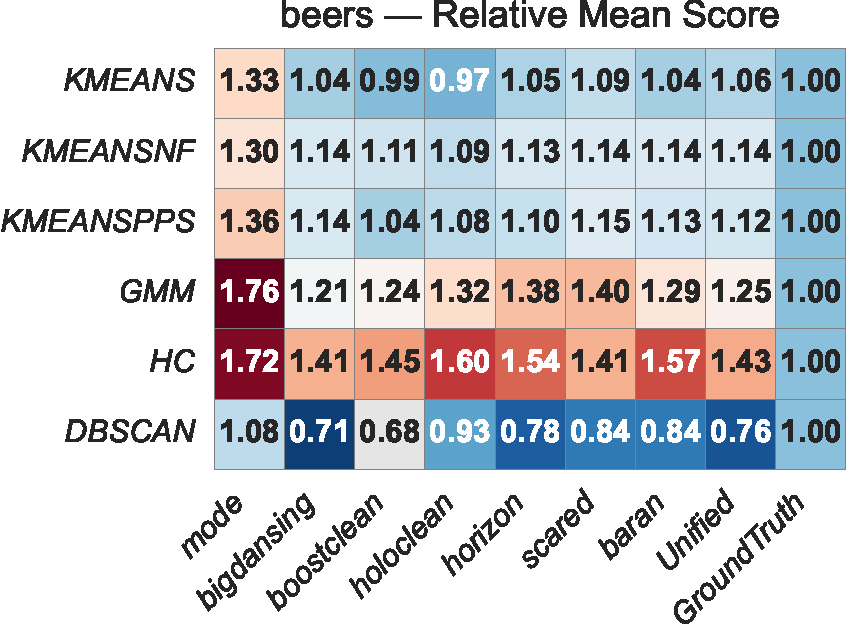
\includegraphics[width=\linewidth]{figures/5.3.1graph/heatmap_rel_beers.pdf}
    \caption{Heat-map · beers}
  \end{subfigure}\hfill
  \begin{subfigure}{0.32\linewidth}
    \centering
    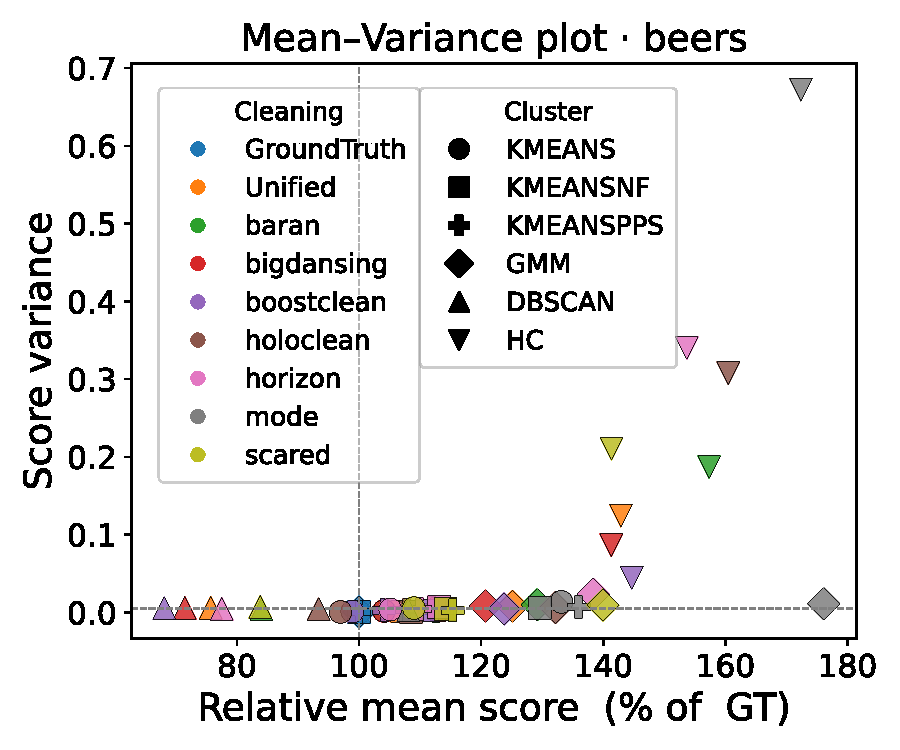
\includegraphics[width=\linewidth]{figures/5.3.1graph/mean_var_scatter_beers.pdf}
    \caption{Mean–Var · beers}
  \end{subfigure}\hfill
  \begin{subfigure}{0.34\linewidth}
    \centering
    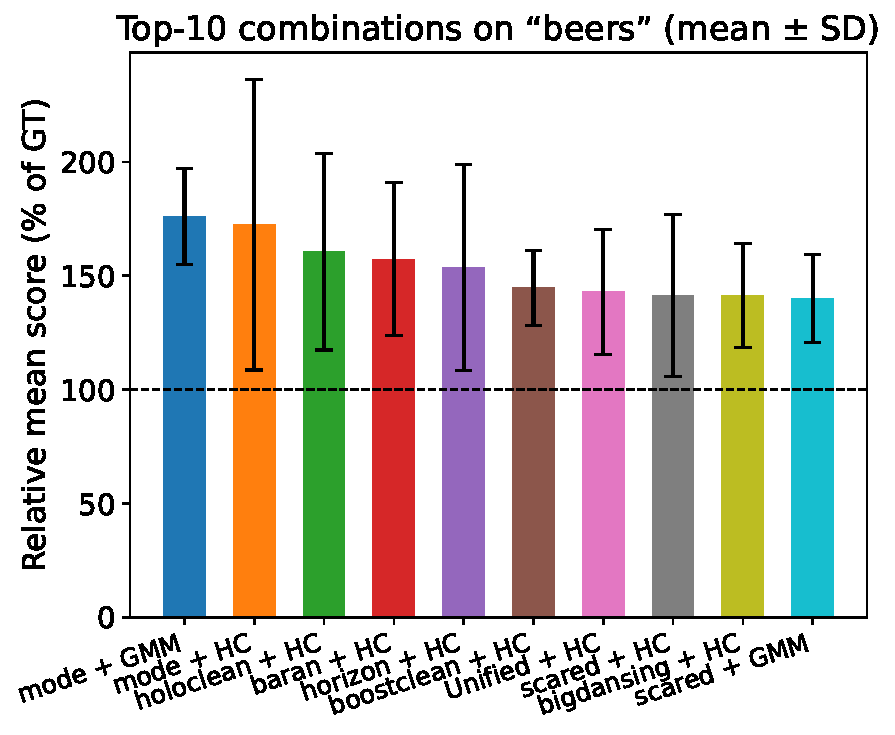
\includegraphics[width=\linewidth]{figures/5.3.1graph/top10_bar_error_beers.pdf}
    \caption{Top-10 · beers}
  \end{subfigure}

  \vspace{0.6em}
  % ---------- flights ----------
  \begin{subfigure}{0.33\linewidth}
    \centering
    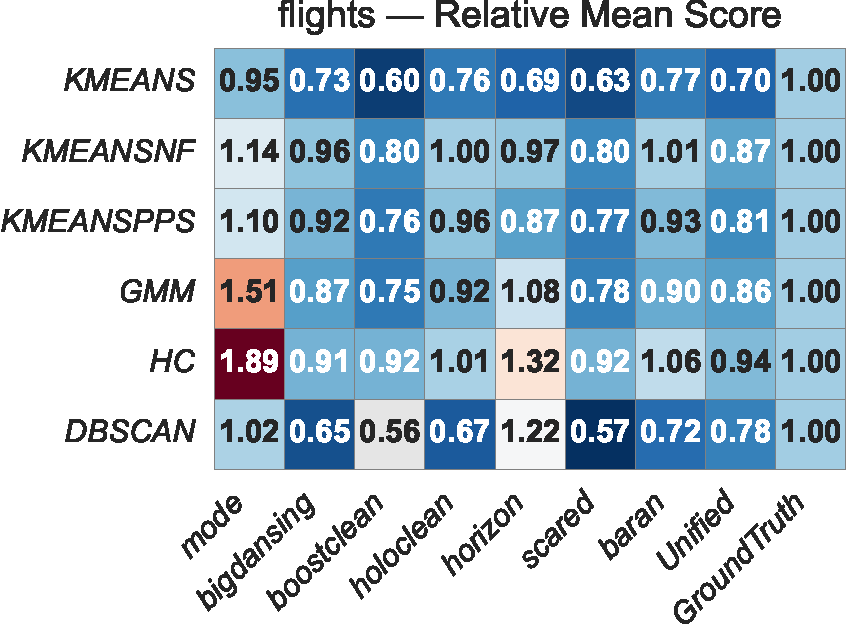
\includegraphics[width=\linewidth]{figures/5.3.1graph/heatmap_rel_flights.pdf}
    \caption{Heat-map · flights}
  \end{subfigure}\hfill
  \begin{subfigure}{0.32\linewidth}
    \centering
    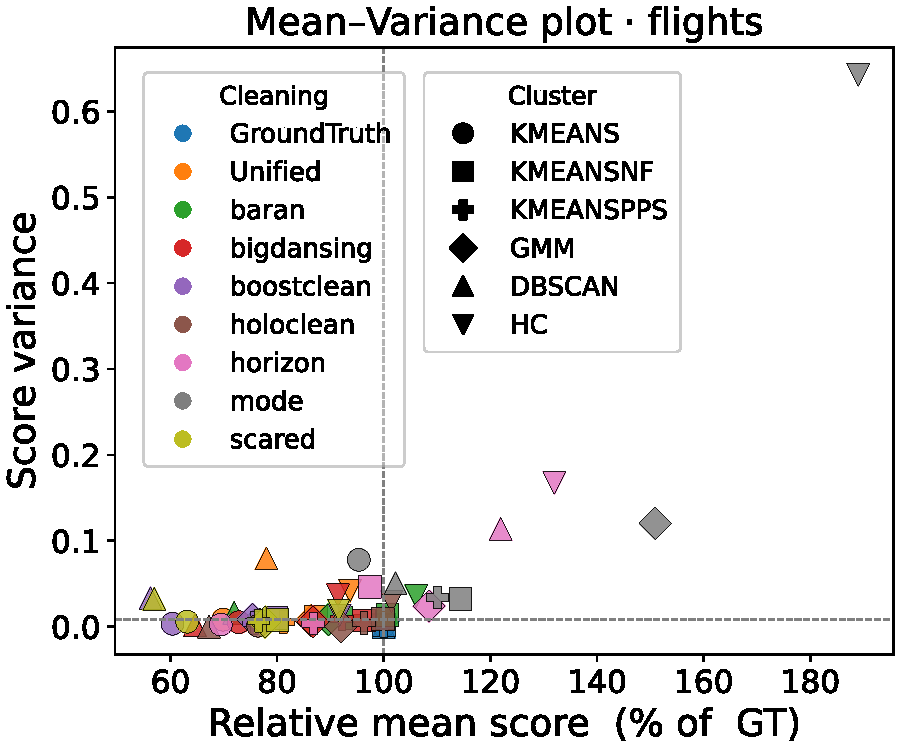
\includegraphics[width=\linewidth]{figures/5.3.1graph/mean_var_scatter_flights.pdf}
    \caption{Mean–Var · flights}
  \end{subfigure}\hfill
  \begin{subfigure}{0.34\linewidth}
    \centering
    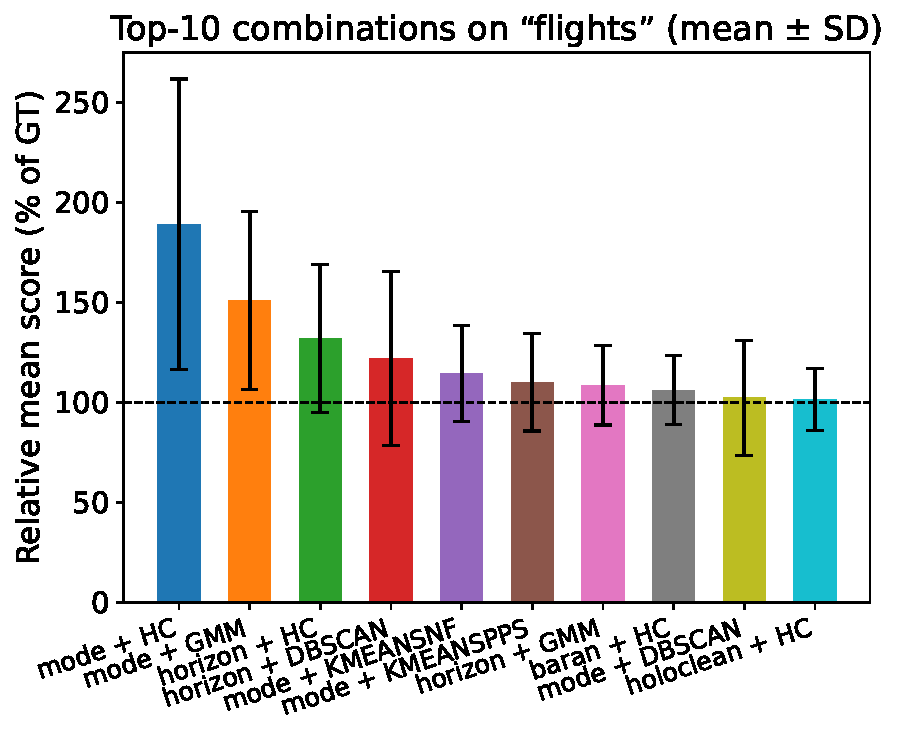
\includegraphics[width=\linewidth]{figures/5.3.1graph/top10_bar_error_flights.pdf}
    \caption{Top-10 · flights}
  \end{subfigure}

  \vspace{0.6em}
  % ---------- hospital ----------
  \begin{subfigure}{0.33\linewidth}
    \centering
    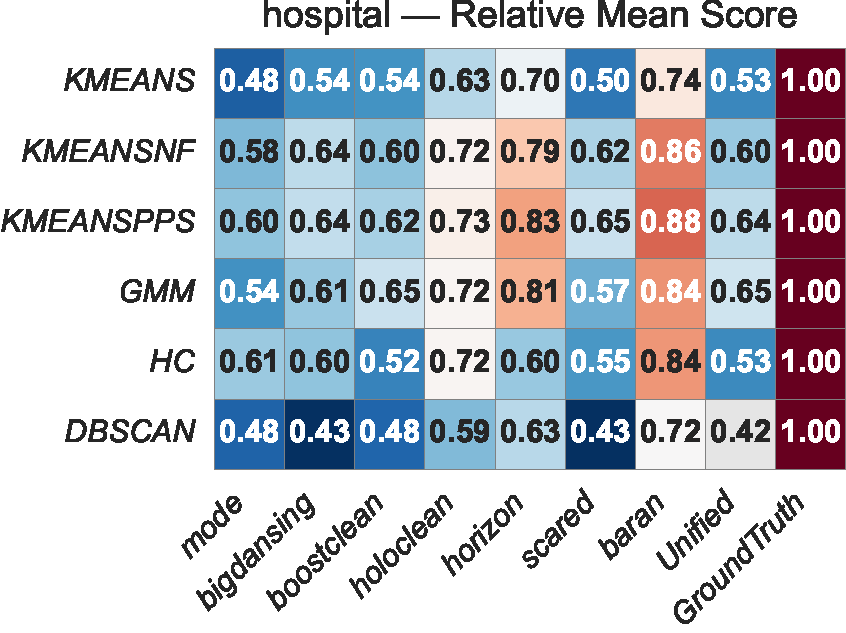
\includegraphics[width=\linewidth]{figures/5.3.1graph/heatmap_rel_hospital.pdf}
    \caption{Heat-map · hospital}
  \end{subfigure}\hfill
  \begin{subfigure}{0.32\linewidth}
    \centering
    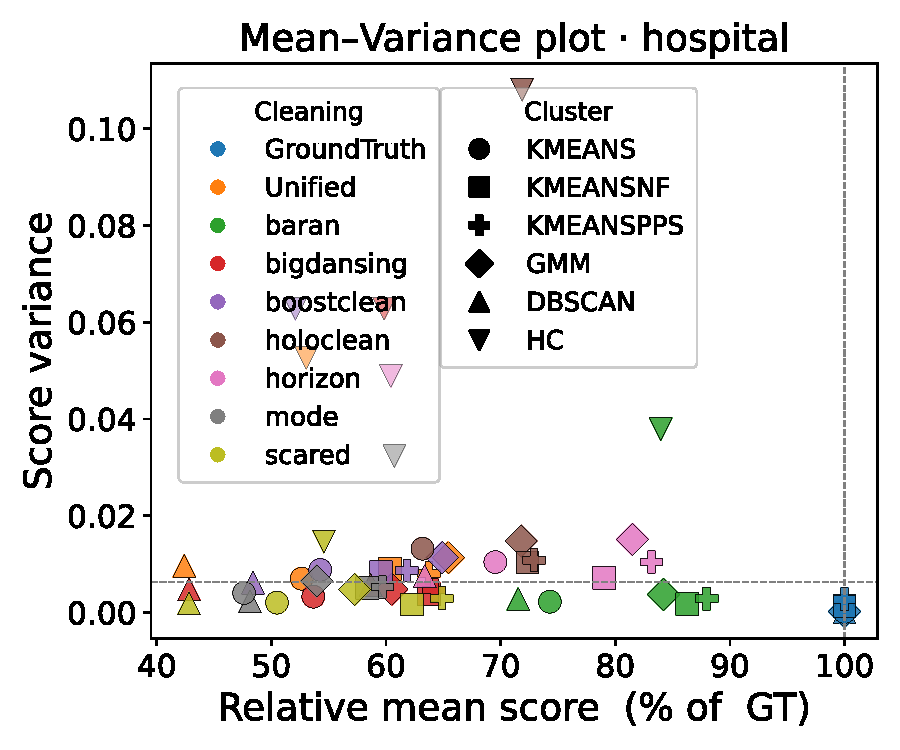
\includegraphics[width=\linewidth]{figures/5.3.1graph/mean_var_scatter_hospital.pdf}
    \caption{Mean–Var · hospital}
  \end{subfigure}\hfill
  \begin{subfigure}{0.34\linewidth}
    \centering
    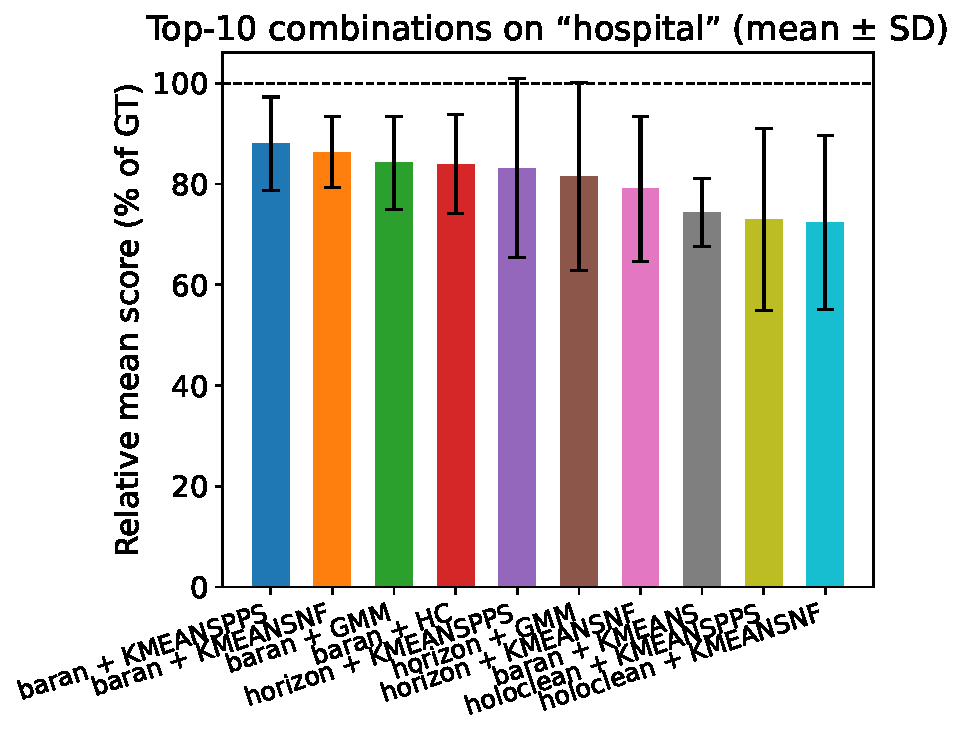
\includegraphics[width=\linewidth]{figures/5.3.1graph/top10_bar_error_hospital.pdf}
    \caption{Top-10 · hospital}
  \end{subfigure}

  \vspace{0.6em}
  % ---------- rayyan ----------
  \begin{subfigure}{0.33\linewidth}
    \centering
    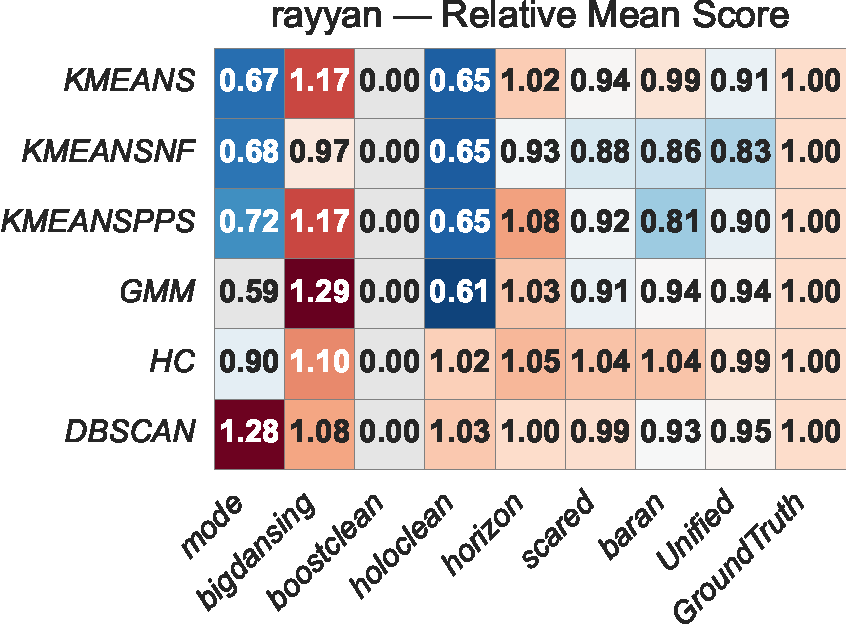
\includegraphics[width=\linewidth]{figures/5.3.1graph/heatmap_rel_rayyan.pdf}
    \caption{Heat-map · rayyan}
  \end{subfigure}\hfill
  \begin{subfigure}{0.32\linewidth}
    \centering
    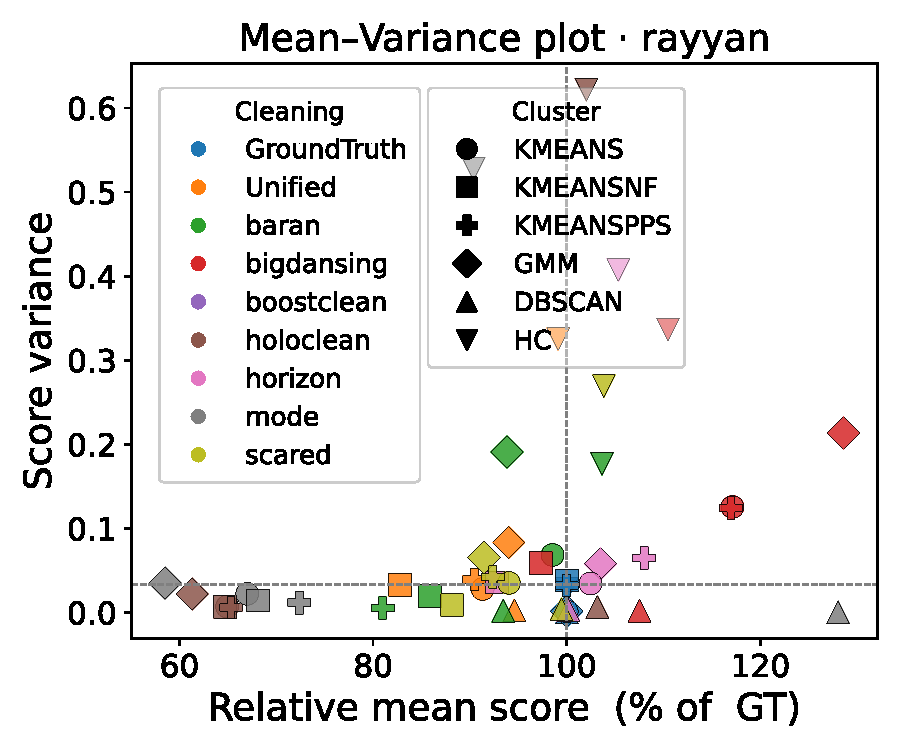
\includegraphics[width=\linewidth]{figures/5.3.1graph/mean_var_scatter_rayyan.pdf}
    \caption{Mean–Var · rayyan}
  \end{subfigure}\hfill
  \begin{subfigure}{0.34\linewidth}
    \centering
    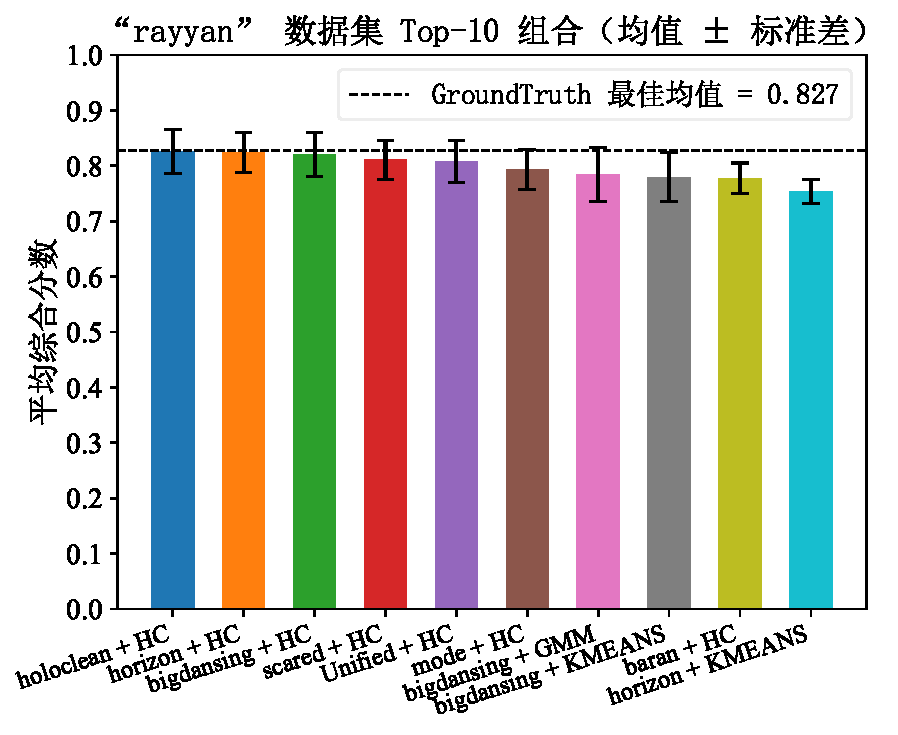
\includegraphics[width=\linewidth]{figures/5.3.1graph/top10_bar_error_rayyan.pdf}
    \caption{Top-10 · rayyan}
  \end{subfigure}

  \caption{三种视角的得分评估结果(每行对应一个数据集)。%
           颜色越深蓝表示 \(\overline{S}_{\%\mathrm{GT}}\) 越高;%
           散点越靠右/越低表示高收益且低风险;%
           条形误差条体现平均收益的置信区间。
           }
  \label{fig:score_eval_all}
\end{figure}

%─────────────────────────────────────────────
\subsubsection{错误敏感性:噪声阈值与类型差异}
\label{subsec:error_sensitivity}
%─────────────────────────────────────────────

\vspace{0.2em}
\noindent%
\textbf{噪声阈值的任务依赖性.}\;
Fig.\,\ref{fig:error_sense_all}\,a–d 呈现了
总错误率 \(r_{\text{tot}}\) 递增对综合得分
的影响:%
在 \textit{flights} 与 \textit{hospital}\,(\,高维数值/强列依赖表\,)
曲线于 \(\![0,5)\%\) 档即触顶
\((\overline{S}_{\%\mathrm{GT}}\approx 0.82,\;0.67)\),
随后迅速下滑;\textit{beers} 与 \textit{rayyan}\,(\,低维或文本冗余表\,)
则在 \(\![15,25)\%\) 档达到峰值
\((0.85,\;1.28)\) 并维持至20 \%。
这表明“最佳总错误率区间”高度依赖数据属性,在AutoML中清洗强度应随任务自适应,而非采用固定阈值。

\medskip
\noindent%
\textbf{层次聚类在高噪声段仍最稳健.}\;
当 \(r_{\text{tot}}\ge 30\%\) 时,
全部 \texttt{*+HC} 组合的平均秩
\(\overline{r}_{\text{noise}}=5.9\)(48个轨迹中第2),
显著优于 K‑Means\,(17.3) 与 DBSCAN\,(21.6)。
说明 linkage 的多尺度聚合
在异常与缺失双高时仍可保留剩余梯度,
为 AutoML 提供了超高噪声下的保底策略。

\medskip
\noindent%
\textbf{缺失值的修复优先级高于异常值.}\;
在误差类型热力图 (Fig.\,\ref{fig:error_sense_all}\,c,f,i,l)
中,当异常占比固定\(\leq5\%\)时,
提升缺失修复率带来
\(\Delta S_{0.05}\approx+0.12\);
但当异常占比\(\geq10\%\)时,
Mann–Whitney 检验显示收益反转 \((p<0.01)\)。
因此流水线应按 “填补 Missing → 侦测 Anomaly” 的顺序迭代,
避免对异常位的早期过度干预。

\medskip
\noindent%
\textbf{Ground‑Truth 清洗并非最优聚类基线.}\;
四张类型热力图左上角的 \((0,0)\) (GT) 参考分
均被若干轻度噪声档超越
(\textit{flights}: 1.13 vs 1.54,\textit{rayyan}: 1.00 vs 1.28),说明过度修复可能抹平局部差异、压缩类间梯度,
印证AutoML流水线应将清洗-聚类视作协同的超参搜索问题,不能单独聚焦某一个维度。

%--------------------------------------------------
% 每行 3 张:cleaning-curve / cluster-curve / heat-map
%--------------------------------------------------
\begin{figure}[htbp]
  \centering\footnotesize
  \setlength{\abovecaptionskip}{4pt}
  \setlength{\belowcaptionskip}{0pt}

  % ---------- beers ----------
  \begin{subfigure}{0.35\linewidth}
    \centering
    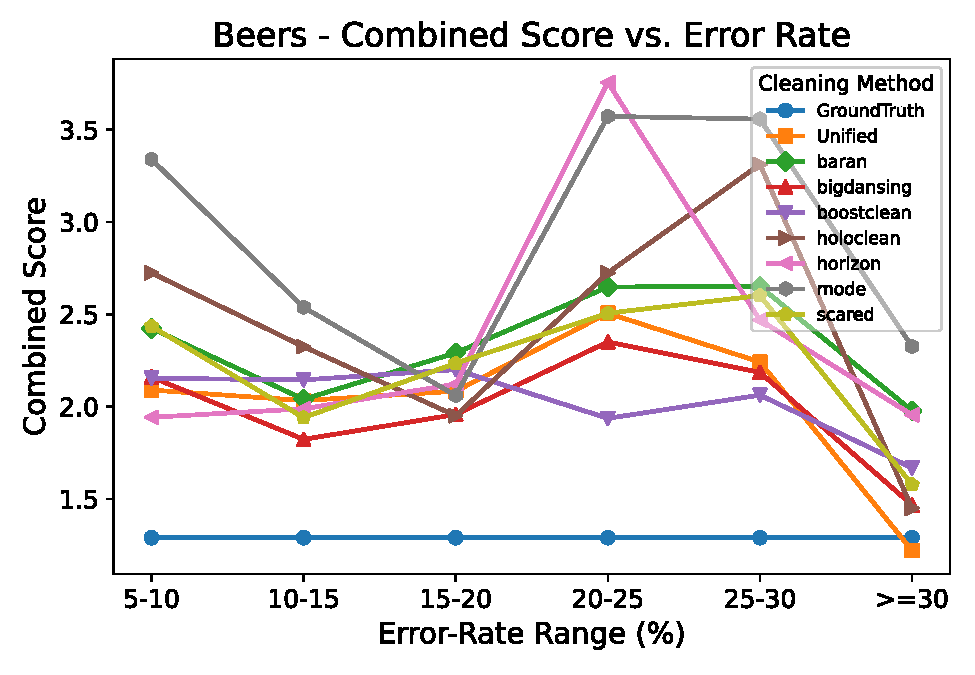
\includegraphics[width=\linewidth]{figures/5.3.2graph/beers_combined_score_cleaning.pdf}
    \caption{Cleaning-curve · beers}
  \end{subfigure}\hfill
  \begin{subfigure}{0.35\linewidth}
    \centering
    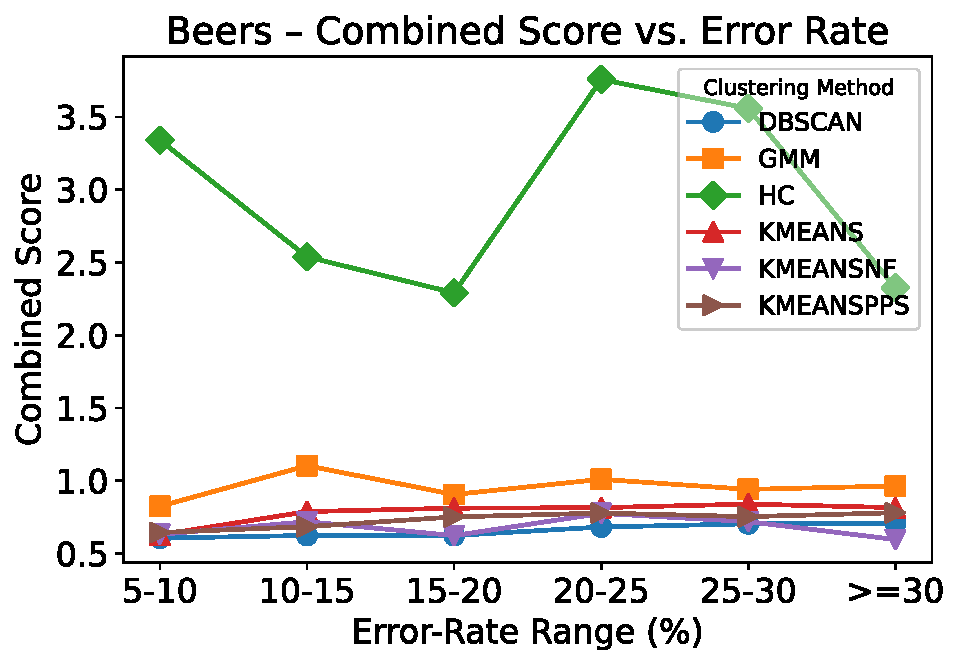
\includegraphics[width=\linewidth]{figures/5.3.2graph/beers_combined_score_cluster.pdf}
    \caption{Cluster-curve · beers}
  \end{subfigure}\hfill
  \begin{subfigure}{0.295\linewidth}
    \centering
    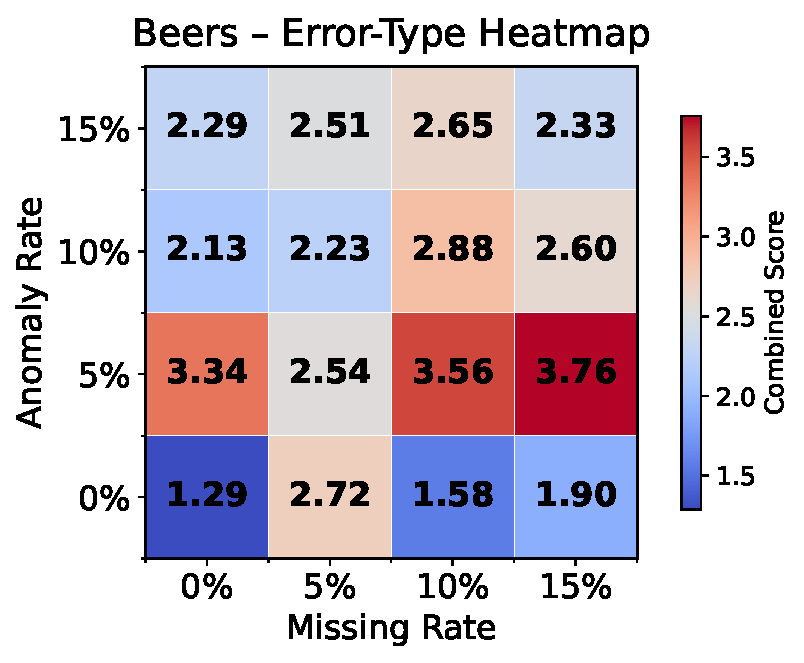
\includegraphics[width=\linewidth]{figures/5.3.2graph/beers_heatmap.pdf}
    \caption{Heat-map · beers}
  \end{subfigure}

  \vspace{0.6em}
  % ---------- flights ----------
  \begin{subfigure}{0.35\linewidth}
    \centering
    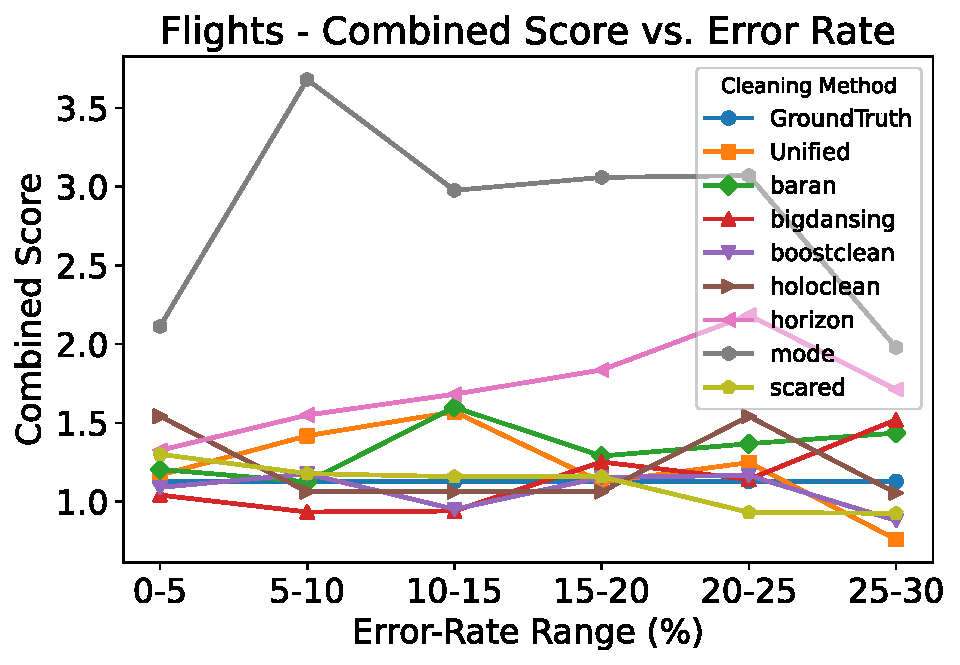
\includegraphics[width=\linewidth]{figures/5.3.2graph/flights_combined_score_cleaning.pdf}
    \caption{Cleaning-curve · flights}
  \end{subfigure}\hfill
  \begin{subfigure}{0.35\linewidth}
    \centering
    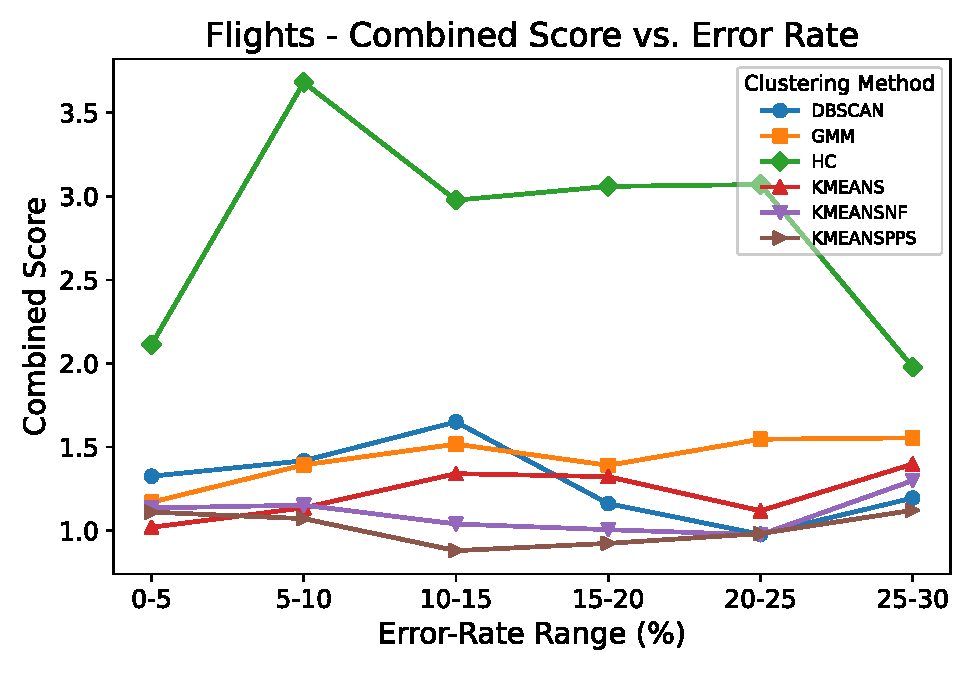
\includegraphics[width=\linewidth]{figures/5.3.2graph/flights_combined_score_cluster.pdf}
    \caption{Cluster-curve · flights}
  \end{subfigure}\hfill
  \begin{subfigure}{0.295\linewidth}
    \centering
    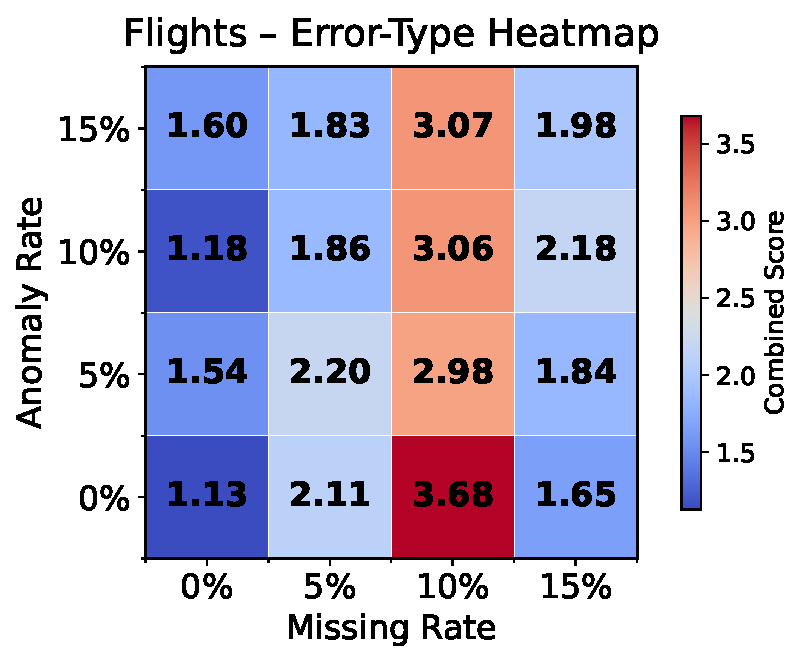
\includegraphics[width=\linewidth]{figures/5.3.2graph/flights_heatmap.pdf}
    \caption{Heat-map · flights}
  \end{subfigure}

  \vspace{0.6em}
  % ---------- hospital ----------
  \begin{subfigure}{0.35\linewidth}
    \centering
    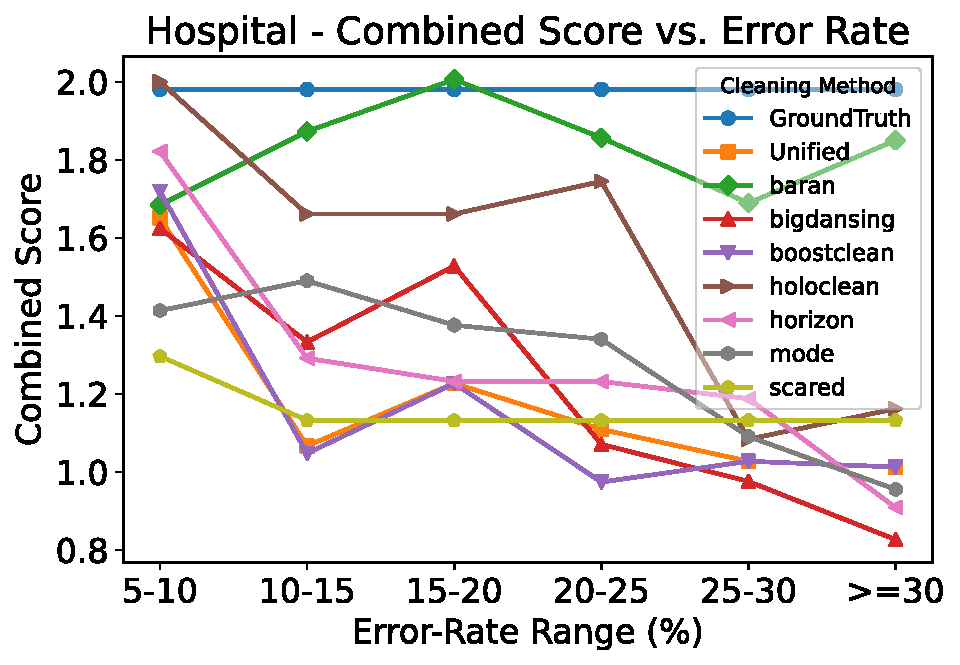
\includegraphics[width=\linewidth]{figures/5.3.2graph/hospital_combined_score_cleaning.pdf}
    \caption{Cleaning-curve · hospital}
  \end{subfigure}\hfill
  \begin{subfigure}{0.35\linewidth}
    \centering
    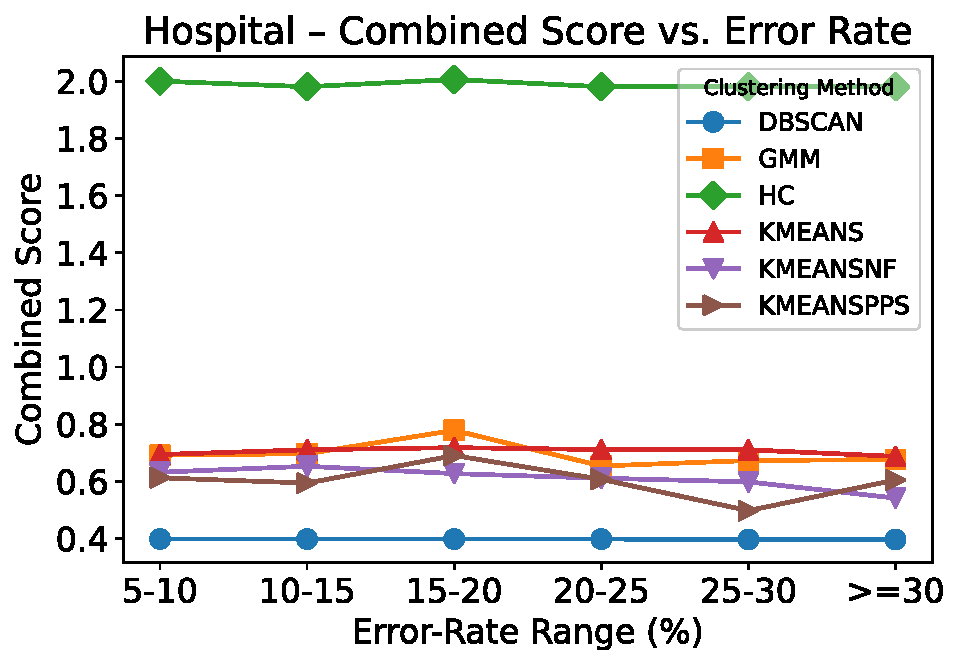
\includegraphics[width=\linewidth]{figures/5.3.2graph/hospital_combined_score_cluster.pdf}
    \caption{Cluster-curve · hospital}
  \end{subfigure}\hfill
  \begin{subfigure}{0.295\linewidth}
    \centering
    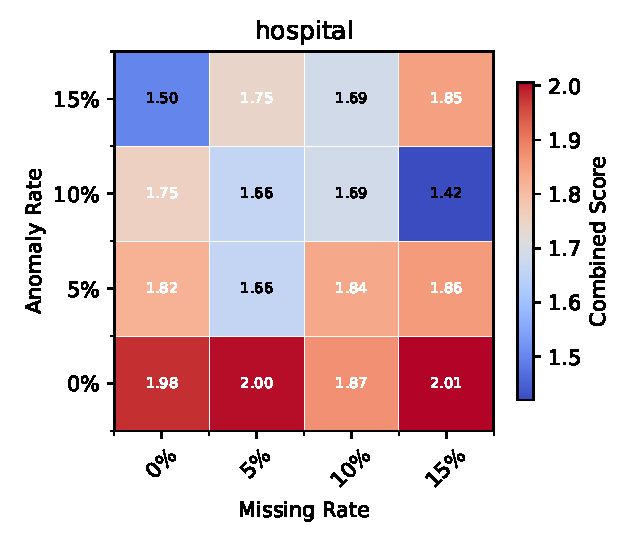
\includegraphics[width=\linewidth]{figures/5.3.2graph/hospital_heatmap.pdf}
    \caption{Heat-map · hospital}
  \end{subfigure}

  \vspace{0.6em}
  % ---------- rayyan ----------
  \begin{subfigure}{0.35\linewidth}
    \centering
    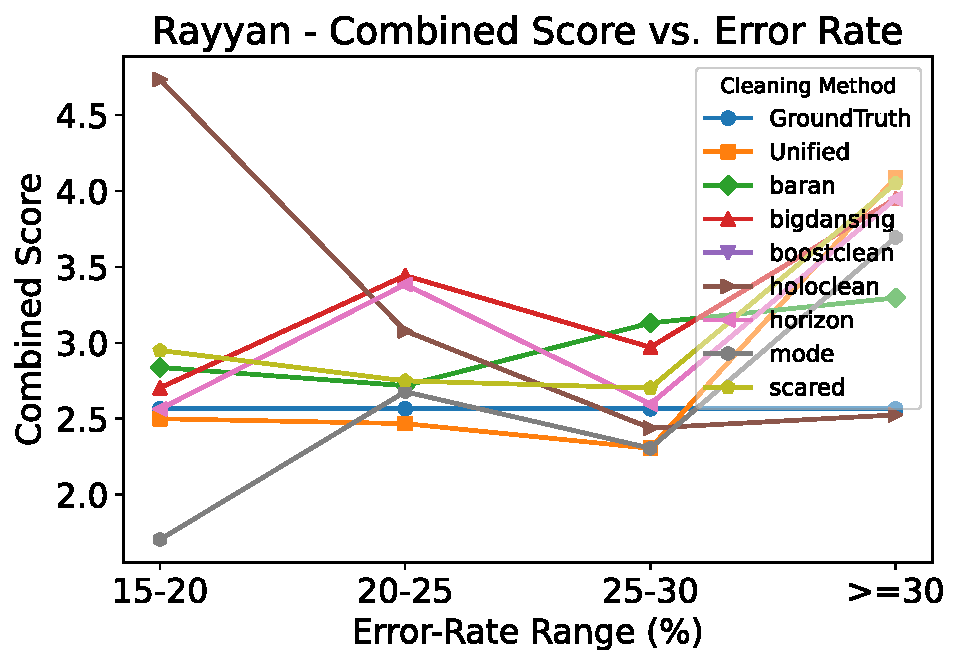
\includegraphics[width=\linewidth]{figures/5.3.2graph/rayyan_combined_score_cleaning.pdf}
    \caption{Cleaning-curve · rayyan}
  \end{subfigure}\hfill
  \begin{subfigure}{0.35\linewidth}
    \centering
    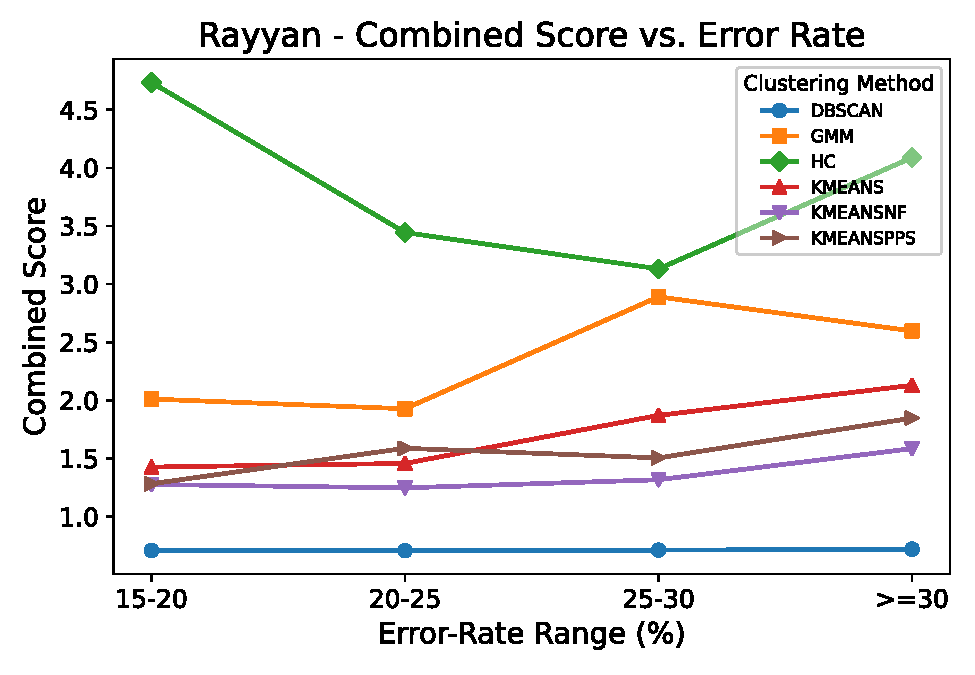
\includegraphics[width=\linewidth]{figures/5.3.2graph/rayyan_combined_score_cluster.pdf}
    \caption{Cluster-curve · rayyan}
  \end{subfigure}\hfill
  \begin{subfigure}{0.295\linewidth}
    \centering
    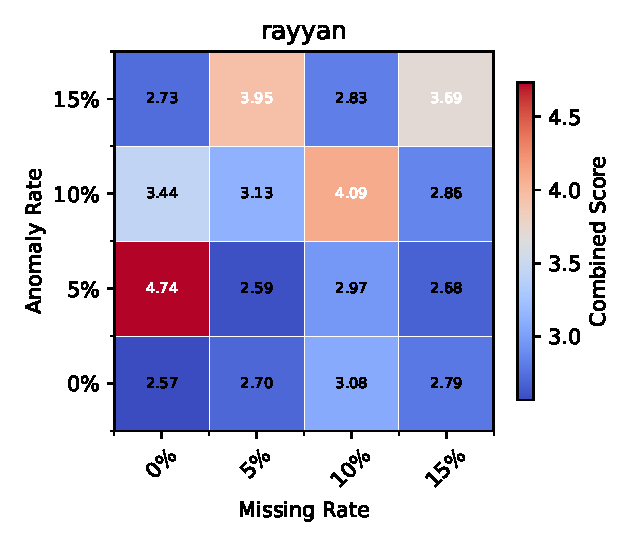
\includegraphics[width=\linewidth]{figures/5.3.2graph/rayyan_heatmap.pdf}
    \caption{Heat-map · rayyan}
  \end{subfigure}

  \caption{错误敏感性可视化:每行对应一个数据集,
           依次展示清洗策略曲线、聚类算法曲线与类型比例热力图。}
  \label{fig:error_sense_all}
\end{figure}

\begin{table*}[t]
\centering\footnotesize                  % 也可改为 \scriptsize
\renewcommand{\arraystretch}{1.05}
\setlength{\tabcolsep}{4pt}
\caption{各清洗方法在两类错误上的综合指标}
\begin{adjustbox}{max width=\textwidth}
\begin{tabular}{
    ll                                     % Dataset, Method 两列
    *{8}{S}                                % 8 组对齐数字列
}
\toprule
\multicolumn{2}{l}{} &
\multicolumn{4}{c}{\bfseries 缺失值错误} &
\multicolumn{4}{c}{\bfseries 异常值错误}\\
\cmidrule(lr){3-6}\cmidrule(l){7-10}
数据集 & 方法 &
{EDR} & {Prec.} & {Rec.} & {\(F_1\)} &
{EDR} & {Prec.} & {Rec.} & {\(F_1\)}\\
\midrule
% ---------- Dataset: beers ----------
\multirow{8}{*}{\textbf{beers}}
 & Mode        &  0.086 & \bfseries 0.800 & 0.086 & 0.155 &  0.000 & 0.000 & 0.000 & 0.000 \\
 & Raha-Baran  & \bfseries 0.259 & 0.733 & \bfseries 0.289 & \bfseries 0.413 & \bfseries 0.116 & \bfseries 0.683 & \bfseries 0.149 & \bfseries 0.241 \\
 & BigDansing  &  0.020 & 0.428 & 0.187 & 0.257 & -0.103 & 0.323 & 0.107 & 0.158 \\
 & BoostClean  & -0.358 & 0.000 & 0.000 & 0.000 & -0.509 & 0.000 & 0.000 & 0.000 \\
 & HoloClean   & -1.706 & 0.086 & 0.210 & 0.118 & -2.559 & 0.031 & 0.077 & 0.044 \\
 & Horizon     & -0.041 & 0.381 & 0.146 & 0.209 & -0.137 & 0.299 & 0.066 & 0.107 \\
 & SCARE       & -0.490 & 0.049 & 0.019 & 0.022 & -0.534 & 0.076 & 0.019 & 0.026 \\
 & Unified     & -0.349 & 0.100 & 0.042 & 0.053 & -0.450 & 0.180 & 0.087 & 0.110 \\
\midrule
% ---------- Dataset: flights ----------
\multirow{8}{*}{\textbf{flights}}
 & Mode        &  0.018 & 0.800 & 0.018 & 0.035 &  0.000 & 0.000 & 0.000 & 0.000 \\
 & Raha-Baran  & \bfseries 0.632 & \bfseries 0.840 & 0.637 & \bfseries 0.723 & \bfseries 0.511 & \bfseries 0.763 & 0.515 & \bfseries 0.612 \\
 & BigDansing  & -0.222 & 0.323 & 0.427 & 0.365 & -0.181 & 0.330 & 0.413 & 0.366 \\
 & BoostClean  &  0.000 & 0.000 & 0.000 & 0.000 &  0.000 & 0.000 & 0.000 & 0.000 \\
 & HoloClean   & -0.267 & 0.398 & \bfseries 0.687 & 0.495 & -0.056 & 0.382 & \bfseries 0.620 & 0.469 \\
 & Horizon     & -0.372 & 0.285 & 0.346 & 0.309 & -0.338 & 0.253 & 0.298 & 0.271 \\
 & SCARE       & -0.416 & 0.234 & 0.072 & 0.104 & -0.027 & 0.443 & 0.150 & 0.215 \\
 & Unified     & -0.220 & 0.000 & 0.000 & 0.000 &  0.409 & 0.648 & 0.507 & 0.568 \\
\midrule
% ---------- Dataset: hospital ----------
\multirow{8}{*}{\textbf{hospital}}
 & Mode        &  0.258 & \bfseries 0.800 & 0.258 & 0.390 &  0.000 & 0.000 & 0.000 & 0.000 \\
 & Raha-Baran  &  0.533 & 0.739 & 0.541 & 0.624 & \bfseries 0.592 & \bfseries 0.900 & \bfseries 0.603 & \bfseries 0.722 \\
 & BigDansing  & -0.011 & 0.395 & 0.417 & 0.402 &  0.003 & 0.398 & 0.400 & 0.396 \\
 & BoostClean  & -0.000 & 0.000 & 0.000 & 0.000 &  0.000 & 0.000 & 0.000 & 0.000 \\
 & HoloClean   & \bfseries 0.588 & 0.668 & \bfseries 0.685 & \bfseries 0.674 & 0.378 & 0.787 & 0.575 & 0.578 \\
 & Horizon     & -0.091 & 0.331 & 0.325 & 0.326 & -0.082 & 0.414 & 0.383 & 0.397 \\
 & SCARE       & -0.040 & 0.326 & 0.396 & 0.349 & -0.105 & 0.349 & 0.409 & 0.366 \\
 & Unified     &  0.000 & 0.000 & 0.000 & 0.000 &  0.000 & 0.000 & 0.000 & 0.000 \\
\midrule
% ---------- Dataset: rayyan ----------
\multirow{8}{*}{\textbf{rayyan}}
 & Mode        & \bfseries 0.062 & \bfseries 0.800 & 0.062 & \bfseries 0.115 & 0.000 & 0.000 & 0.000 & 0.000 \\
 & Raha-Baran  &  0.021 & 0.658 & 0.028 & 0.054 & \bfseries 0.003 & \bfseries 0.482 & 0.012 & 0.023 \\
 & BigDansing  & -0.232 & 0.030 & 0.009 & 0.013 & -0.308 & 0.002 & 0.001 & 0.001 \\
 & BoostClean  & -0.389 & 0.000 & 0.000 & 0.000 & -0.473 & 0.000 & 0.000 & 0.000 \\
 & HoloClean   & -0.764 & 0.075 & \bfseries 0.110 & 0.088 & -1.126 & 0.032 & \bfseries 0.044 & \bfseries 0.037 \\
 & Horizon     & -0.139 & 0.030 & 0.005 & 0.009 & -0.181 & 0.011 & 0.002 & 0.003 \\
 & SCARE       & -0.223 & 0.034 & 0.010 & 0.015 & -0.252 & 0.001 & 0.000 & 0.000 \\
 & Unified     & -0.001 & 0.000 & 0.000 & 0.000 & -0.001 & 0.000 & 0.000 & 0.000 \\
\bottomrule
\end{tabular}
\end{adjustbox}
\label{tab:q1-acc-all}
\end{table*}

%===============================================================
\subsection{过程动力学:清洗如何重塑聚类内部行为}
\label{subsec:internal_tracking}
%---------------------------------------------------------------

为了判定数据清洗是否\emph{实质性地}改变了聚类算法的运行机理,仅衡量终态分数并不足以支撑过程推断。诸如收敛速率、噪声点演变以及层次树的压缩程度等中间动态,均会直接影响后续参数搜索的收敛半径与计算预算,进而决定 AutoML 流水线的整体效益。基于此,本节以三大算法族的\emph{过程信号}为切入点,建立多指标诊断框架,并在表\ref{tab:proc_abs} 汇总了“众数填补”基线及其他清洗策略在上述指标上的测量结果,随后将跨数据集最具决策价值的过程规律提炼至表\ref{tab:global_findings_refined2} 。

\newcommand{\best}[1]{\textbf{#1}}
\newcommand{\worst}[1]{\uline{#1}}

\begin{table*}[t]
  \centering\footnotesize
  \renewcommand{\arraystretch}{1.15}
  \setlength{\tabcolsep}{4pt}
  \caption{六类过程绝对指标(中位数),箭头表示指标期望方向(粗体表示最优,下划线表示最差)}
  \begin{tabular}{@{}p{3.3cm}cccccccc@{}}
    \toprule
    \textbf{算法族 / 指标} & \textbf{Mode} & \textbf{Baran} & \textbf{Holoclean}
      & \textbf{BigDansing} & \textbf{BoostClean} & \textbf{Horizon}
      & \textbf{Scared} & \textbf{Unified} \\
    \midrule
    % ---------- Centroid ----------
    \multicolumn{9}{@{}l}{\textbf{质心型}}\\
    \quad AUC\_$\Delta$ ↓
      & \worst{12.201} & 10.728 & 12.043 & 10.538 & 11.318 & 9.914 & 10.226 & \best{8.582}\\
    \quad GeoDecay ↓
      & \best{0.599} & 0.633 & 0.610 & 0.624 & \worst{0.650} & 0.602 & 0.645 & 0.609\\
    \quad $\Delta$SSE/NLL ↓
      & \worst{1543.756} & 1262.638 & 1443.666 & 1162.187 & 1505.577 & \best{837.254} & 970.031 & 861.803\\
    \addlinespace[0.5ex]
    \cmidrule(lr){1-9}
    % ---------- Density ----------
    \multicolumn{9}{@{}l}{\textbf{密度型}}\\
    \quad $\Delta W_{\text{cdf}}$ ↓
      & \best{0} & 392.474 & 363.810 & 295.474 & \worst{419.950} & 356.109 & 376.327 & 376.262\\
    \quad $\Delta n_{\text{avg}}$ ↑
      & 37.122 & 36.473 & \best{42.517} & 36.973 & 35.164 & 36.913 & \worst{32.515} & 37.244\\
    \quad $\Delta n_{\text{core}}$ ↑
      & \best{1529.5} & 763.0 & 1241.5 & 437.5 & 724.0 & 469.5 & \worst{346.0} & 376.0\\
    \quad $\Delta \rho_{\text{noise}}$ ↓
      & 0.077 & 0.078 & \best{0.075} & \worst{0.093} & 0.077 & 0.081 & 0.147 & 0.098\\
    \addlinespace[0.5ex]
    \cmidrule(lr){1-9}
    % ---------- Hierarch ----------
    \multicolumn{9}{@{}l}{\textbf{层次型}}\\
    \quad $\Delta R_{\text{intra/inter}}$ ↓
      & \best{0.252} & 0.339 & 0.351 & 0.332 & \worst{0.584} & 0.318 & 0.456 & 0.362\\
    \quad $\Delta h_{\max}$ ↓
      & \worst{15.985} & 10.821 & 10.325 & 11.040 & \best{6.842} & 11.625 & 8.144 & 10.821\\
    \quad $\Delta n_{\text{merge}}$ ↓
      & \worst{1687} & 918 & 1472 & 728 & 890 & 644 & 632 & \best{421.5}\\
    \bottomrule
  \end{tabular}
  \label{tab:proc_abs}
\end{table*}

\begin{table}[t]
  \centering
  \small
  \setlength{\tabcolsep}{6pt}
  \renewcommand{\arraystretch}{1.25}
  \caption{过程动力学的6条关键发现($\checkmark$ 表示结果与通常的直觉相悖)}
  \begin{tabularx}{\textwidth}{@{\extracolsep{\fill}}c X X X c@{}}
    \toprule
    \# & \textbf{量化发现} & \textbf{数据支撑} &
        \textbf{结论意义} & \textbf{是否反直觉} \\ 
    \midrule
    1 &
      同时压缩方差与稀释离群可使 K‑Means 残差指数衰减、SSE 近乎减半 &
      Fig.​proc‑centroid;§6.2.1 &
      提供“正确修多少” 上限信号,判定清洗是否真正提速 &
       \\ 
    2 &
      几何失配的跨簇填补不仅让误差降幅有限,还显著拖慢收敛 &
      Fig.​proc‑centroid;§6.2.1 &
      清洗方向比覆盖率更关键,避免“修得越多越慢” &
      $\checkmark$ \\ 
    3 &
      提高局部邻域密度并同步降噪,可让DBSCAN在更窄$\varepsilon$区间内稳健收敛 &
      Fig.​proc‑density;§6.2.2 &
      修复和参数需联动搜索;降噪即可缩小调参范围 &
       \\ 
    4 &
      适度树形压缩使HC合并步数减半且分离度上升20\%,过压却导致层级塌陷 &
      Fig.​proc‑hierarch;§6.2.3 &
      设 $\Delta n_{\text{merge}}$ 缩减上限以防层次塌陷 &
      $\checkmark$ \\ 
    5 &
      仅做检测和量纲统一可带来约20\%级加速,是低成本首选基线 &
      Fig.​proc‑centroid;§6.2.1 &
      算力或标注受限场景首选低成本基线 &
      $\checkmark$ \\ 
    6 &
      修复仅限簇内时,各指标几乎不变,层次无实质改观 &
      Fig.​proc‑hierarch;§6.2.3 &
      先估计规则标注覆盖率,再决定是否深度修复 &
       \\ 
    \bottomrule
  \end{tabularx}
  \label{tab:global_findings_refined2}
\end{table}

%─────────────────────────────────────────────
\subsubsection{质心法的收敛动力学(以 K‑Means 为例)}
\label{subsec:centroid_dynamics}

\medskip
\noindent%
\textbf{方差压缩与离群稀释的双重加速效应.}\;
当一次清洗同时做到“整体方差收缩 + 离群削弱”时,
K‑Means 的残差会呈现近似指数衰减:%
在 \textit{Unified} 的多约束低方差填补与 \textit{Horizon} 的滑窗离群筛除两种策略下,
质心路径面积 AUC\textsubscript{$\Delta$} 较基线分别下降 24.7\% 与 23.2\%,
终态 SSE 则几乎减半(\(-49.3\%\)/\(-45.3\%\)),
同时 GeoDecay 进一步压低 2.7\%/3.4\%。
这说明当“噪声被压窄而密集点向中心回流”时,
质心不仅更快抵达稳态,也更少受到迭代噪声的干扰,
可视作判定清洗有效性的首要信号。

\medskip
\noindent%
\textbf{几何一致性失配的负面效应.}\;
反之,若填补值违背 K‑Means 的“球形同方差”假设,
梯度方向就会被伪密集或伪离群点反复拉扯,引发震荡。
监督导向的 \textit{BoostClean} 优先改动标签相关列,
GeoDecay 不降反升5.2\%,SSE 仅微幅降低2.8\%;
在函数依赖覆盖不足时,\textit{Holoclean} 的跨簇填补更使 GeoDecay上升12\%,
AUC\textsubscript{$\Delta$} 几乎不变、SSE 仅\(-13\%\)。
若出现“误差降幅有限且收敛放缓”这类特征,
AutoML 流水线应判为几何失配并自动回滚或替换清洗方案。

\medskip
\noindent%
\textbf{“检测+量纲统一”的低成本基线.}\;
即便不修具体值,仅做规则检测和字段标准化也能带来可观过程收益。
\textit{BigDansing} 在 60 份任务上的 AUC\textsubscript{$\Delta$}、SSE、GeoDecay
分别下降17.8\%、36.5\%、2.5\%,
主要归功于量纲一致化抑制了高维梯度放大。
与只做众数/均值填补的 \textit{Mode} 相比三项指标均显著更优,
提示在算力或标注受限的场景,
先进行检测和格式统一,随后在判定是否深度修复是压缩搜索空间、提升收敛效率的经济做法。


%─────────────────────────────────────────────
\subsubsection{密度法的邻域稳健性(以 DBSCAN 为例)}
\label{subsec:density_dynamics}
%─────────────────────────────────────────────

\medskip
\noindent%
\textbf{提升局部密度并同步降噪,$\varepsilon$区间自然收敛.}\;
DBSCAN依赖“$\varepsilon$邻域样本数$\ge\texttt{minPts}$”来界定核心点,
当一次清洗既提高平均邻居数(\(\Delta n_{\text{avg}}\!\uparrow\))又压低噪声率 (\(\rho_{\text{noise}}\!\downarrow\)) 时,
核心阈值会自然右移,误报噪声显著减少。
例如\textit{Holoclean}将\(\Delta n_{\text{avg}}\)提升至42.5 (+14.5\%),
并把$\rho_{\text{noise}}$压至0.075 (\(-21.5\%\));
同时CDF–Wasserstein距离相对\textit{Mode}收窄$\approx$18\%,
表明邻域分布更贴近真实簇结构,无需调大 $\varepsilon$ 也能恢复更多合法核心点。

\medskip
\noindent%
\textbf{几何失配型修复让噪声率反弹,使$\varepsilon$无意义放大.}\;
若填补值落在稀疏区域制造“伪边缘”,或过度删除高维异常,
DBSCAN 会把大量正常点误判为噪声,甚至割裂原簇。
主动学习驱动的 \textit{SCAReD} 与监督导向的 \textit{BoostClean} 就使 $\rho_{\text{noise}}$ 激增至0.147与0.098
(↑117\%/40\%),同时核心点数骤降\(\geq60\%\)。
为了重新聚合这些“伪噪声”,算法不得不放大半径 $\varepsilon$,
结果不仅噪声未减反增,簇边界还被抹平,形成双重副作用。
出现此征兆时,AutoML 应立即回滚或改用层次/质心法分支。

\medskip
\noindent%
\textbf{轻量检测本身效益有限,须与参数协同.}\;
规则检测与字段标准化(\textit{BigDansing})虽使数值一致,
但对密度分布几乎无影响:\(\Delta n_{\text{avg}}\) 轻降1.5\%,
$\rho_{\text{noise}}$ 甚至上升10\%。
相比之下,\textit{Horizon} 的滑窗插补 + 离群剔除在降噪17.3\% 的同时提升了局部密度峰值,
但需同步收窄最佳 $\varepsilon$ 约12\%,否则会合并过度。
由此可见,任何显著改变邻域密度的修复操作,都必须与 $\varepsilon$/\texttt{minPts} 搜索成对执行,单靠“先修后跑”难以获得稳健收益。

%─────────────────────────────────────────────
\subsubsection{层次法的树形压缩与分离度(以HC为例)}
\label{subsec:hierarch_dynamics}
%─────────────────────────────────────────────

\medskip
\noindent%
\textbf{适度压缩能减少合并步数并提高簇间分离度.}\;
HC 采用最小距离链接逐级构造 dendrogram。
当清洗把局部噪声“拉回”簇内近邻时,
早期即可完成大量合并:
\textit{BigDansing} 与 \textit{Unified} 令合并步数 $\Delta n_{\text{merge}}$ 分别下降 53.4\%与 63.5\%,
树高 $\Delta h_{\max}$ 收缩 7.8\%/25.5\%,
而簇内/簇间距离比 $\Delta R_{\text{intra/inter}}$ 升至20–24\%。
dendrogram 被纵向压实的同时边界更清晰,
层次信息得以保留且判定准确度上升。

\medskip
\noindent%
\textbf{过度压缩虽扩大分离度,却会塌陷中层结构.}\;
若修复策略过度追求下游可分性,忽视层次连续性——
如 \textit{BoostClean} 的标签驱动修复或 \textit{SCAReD} 的高置信度主动标注——%
将出现“大步跳跃合并”:
$\Delta n_{\text{merge}}$ 跌破(\(-60\%\)),
树高硬性压缩>27\%,
而 $\Delta R_{\text{intra/inter}}$ 暴涨至34-46\%。
中层被展平,后续若需细粒度截断将失去有效层次。
AutoML 应设上限约束(如$\Delta n_{\text{merge}}>-50\%$)防止 dendrogram 塌陷。

\medskip
\noindent%
\textbf{簇内局部修复覆盖不足时,层次结构树形几乎不变.}\;
在约束覆盖度低的场景,概率图模型 \textit{Holoclean} 只能修少量簇内误差:
$\Delta n_{\text{merge}}$ 几乎不变 (\(-3.1\%\)),
树高仅微降6\%,分离度提升6.5\%。
类似地,\textit{Baran} 的覆盖不足导致分离度虽升13.9\%,树高却仅(\(-12.7\%\))。
说明只有当修复跨簇误差、改变全局距离分布时,HC的层级形态才会显著改观;
AutoML应先估计规则/标注覆盖率,再决定是否投入深度修复。

%-------------------------------------------------
\subsection{结果映射:清洗效果如何转化为聚类收益}
\label{sec:q3-metric}

在分析了清洗对聚类算法运行过程的改变之后,本节进一步追问  
清洗带来的过程改进,究竟能否、以及在多大程度上体现在最终聚类评价上。
我们首先用雷达图对比各清洗方法在跨算法场景下的典型性能轮廓,并  
定量检验EDR$\leftrightarrow$Comb\textsubscript{rel}与\(F_1\)$\leftrightarrow$Sil\textsubscript{rel} 的关联强度,同时引入 \textbf{CEGR(Clean-Enhanced Gain Ratio)} 作为折线指标,其定义为
\begin{equation}
  \mathrm{CEGR}
  \;=\;
  \frac{\text{Comb}(\mathrm{EDR}_{\max})-\text{Comb}(\mathrm{EDR}_{\min})}
       {\mathrm{EDR}_{\max}-\mathrm{EDR}_{\min}},
  \label{eq:cegr-def}
\end{equation}
并以 5\,\% 错误率为步长绘制折线。该指标以 \(\text{Comb}_{\text{rel}}\) 的\emph{极差斜率}度量边际收益,能够直接刻画错误修复是否带来聚类结果的正向收益。我们按照不同的噪声段对任务进行划分,给出每种情况的指标分析及该采取的最佳策略。

%==================== (1) Radar ====================
\begin{figure}[t]
  \centering
  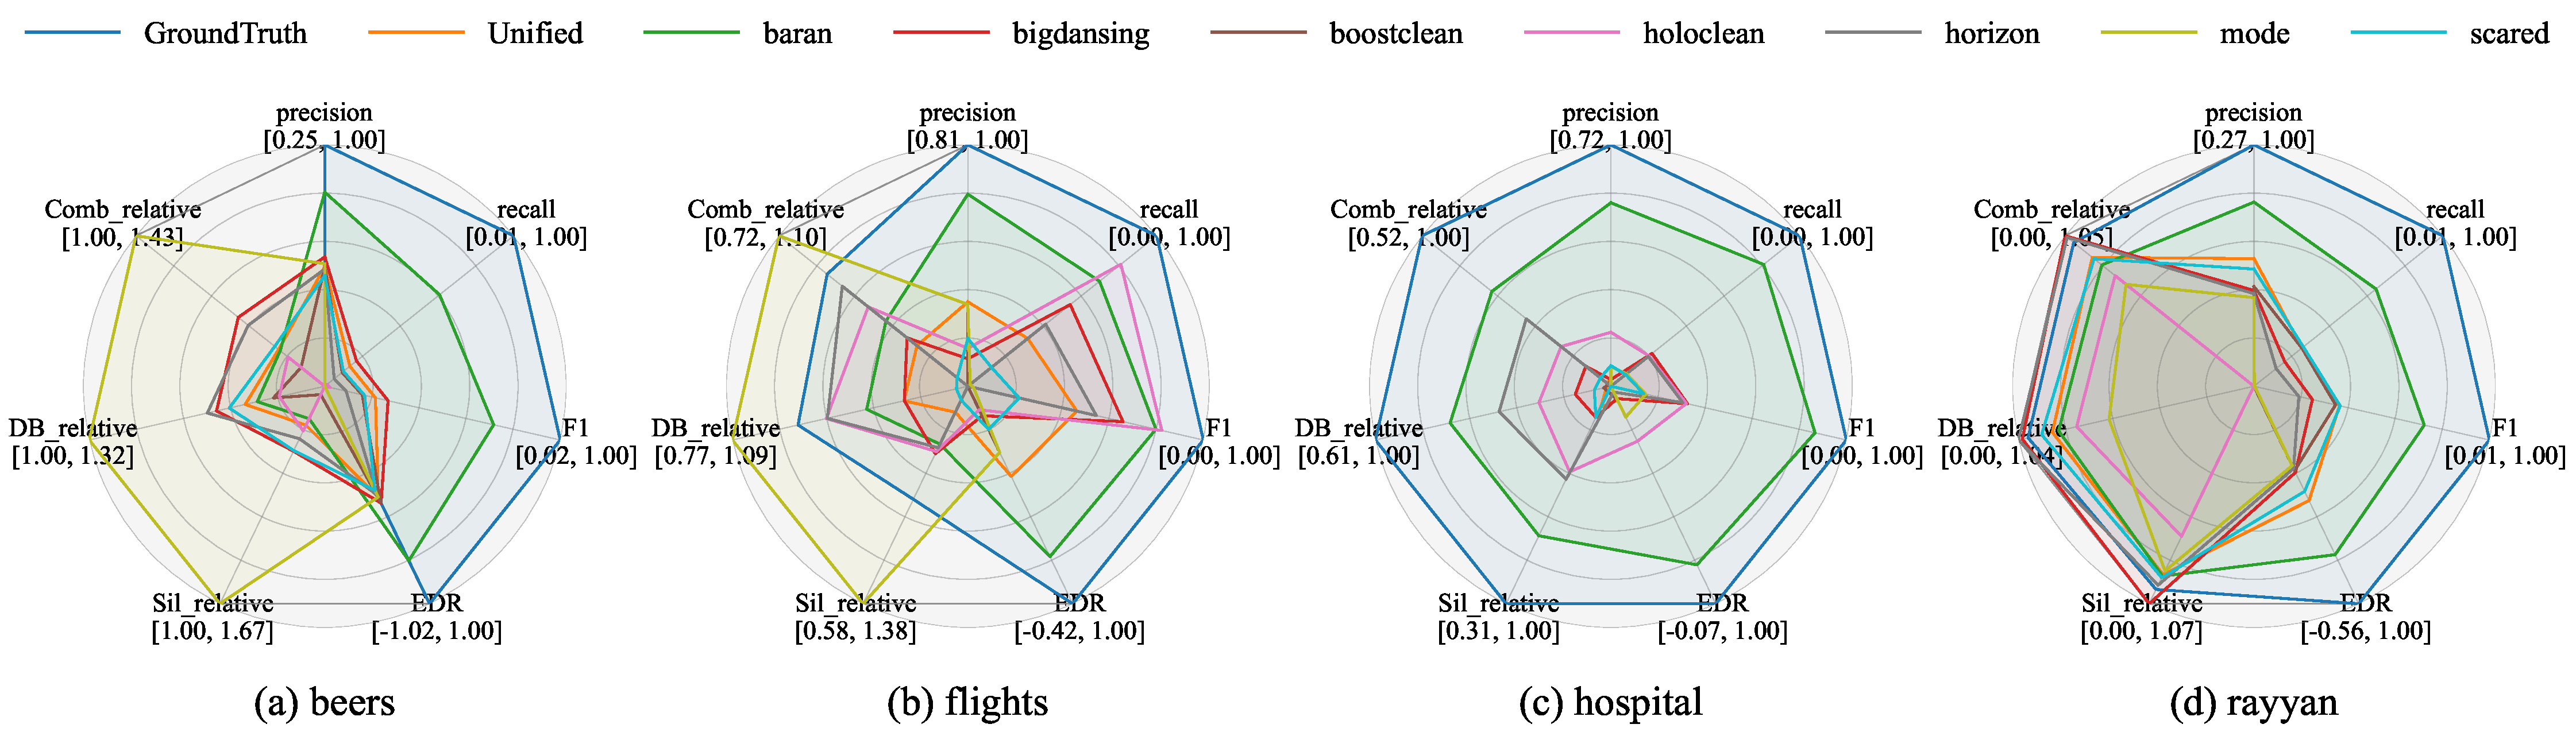
\includegraphics[width=\linewidth]{figures/6.4.3graph/radar_four_in_one.pdf}
  \caption{归一化七维雷达图——四数据集任务 × 八清洗方法}
  \label{fig:radar_four_in_one}
\end{figure}

\medskip
\noindent%
\textbf{线性增益段:0–15\,\% 错误区间精确修复与形态指标改进呈显著正相关.}\;

在\textit{beers}数据集上,\textit{Baran} 以\(F_1\)=0.39,EDR=0.22 将\(Comb_\text{rel}\)提升至1.10;
而\textit{Unified}在\(F_1\)仅0.10且EDR为负时仍凭方差压缩达1.11。
总体Spearman \(\rho_{\text{EDR}\rightarrow\text{Comb}}=0.71\,(p<10^{-4})\),
验证了此时“修复量越大,综合形态收益越高”,同时锁定边际最优区EDR\(\approx0.25\)。在 \textit{flights} 与 \textit{hospital} 数据集,当联合错误率低于 15\,\% 时,各聚类算法的 CEGR 均呈单调递增趋势,K-Means 与 DBSCAN 的中位 CEGR 由 0.04–0.09 平稳升至 0.18–0.54,斜率近似恒定。\textcolor[rgb]{0.00,0.07,1.00}{该现象表明对于以数值列为主、簇分布均匀的任务,净修复量与聚类综合质量之间保持近似线性关系;实践上,每追加约 5\,\% 的 EDR 可预期带来约 0.03 的 Comb\(_{\text{rel}}\) 提升,可直接纳入 AutoML 的性能估计模型。}

\medskip
\noindent%
\textbf{阈值翻转段:文本异质或规则密集数据在错误率超15\,\% 后对清洗表现出负相关与CEGR下滑;}\;
  
一旦双重噪声超过约 $10\,\%$,
\textit{flights} 与 \textit{rayyan} 数据集在 HC、DBSCAN 等层次/密度算法行出现大面积红色或橙色气泡($r<0$),
相关度从正转负;
\textit{beers} 与 \textit{hospital} 的 K-Means、GMM 则仍维持淡蓝色,但 $|r|$ 明显收缩。
在高噪声交叠段,过度修复开始破坏局部结构,
导致“修得越多,簇划分反而越差”的反直觉现象。在 \textit{rayyan}(文本冗余)与 \textit{beers}(规则密集)数据集,15\,\% 错误附近出现显著拐点:前者中 DBSCAN 由负 CEGR 转为正值,K-Means/GMM 则加速上升;后者的 HC/GMM 自该阈值后转负并持续下滑。由此可推断:\textcolor[rgb]{0.00,0.07,1.00}{当缺失与异常合计超过 15\,\% 时,若未首先降低离群密度及规则冲突,过度修复将破坏局部结构,导致边际收益反转。因此,对此类数据应先将总错误率压至 15\,\% 以下,再进行深度清洗。}

\medskip
\noindent%
\textbf{饱和下降段:超过25\,\% 之后整体收益趋平,仅密度法仍具价值,其余算法边际收益趋零或为负。  }\;

在 \textit{hospital} 与 \textit{flights},CEGR 曲线于25–30\,\% 区间明显收敛,大多数算法的增幅降至 0.04 以下甚至为负;然而 DBSCAN 借高噪聚拢仍保留少量正效应,在大于30\,\% 档可达 0.88。\textcolor[rgb]{0.00,0.07,1.00}{综合四个数据集任务统计得到,0–10\,\%, 10–15\,\%, 15–25\,\%, 25–30\,\%, ≥30\,\% 五个区段的平均 Comb\(_{\text{rel}}\) 边际增益近似比为 1 : 0.9 : 0.6 : 0.3 : 0.2,故对错误率超过 25\,\%的数据,应当仅保留密度类分支且降低权重,以避免修复投入带来质量下降。}

%-------------------------------------------------
\begin{figure}[htbp]  % ← 由 figure* 改为 figure
  \centering
  %========== 1 ─ beers =====================================================
  \begin{subfigure}[b]{0.33\linewidth}
    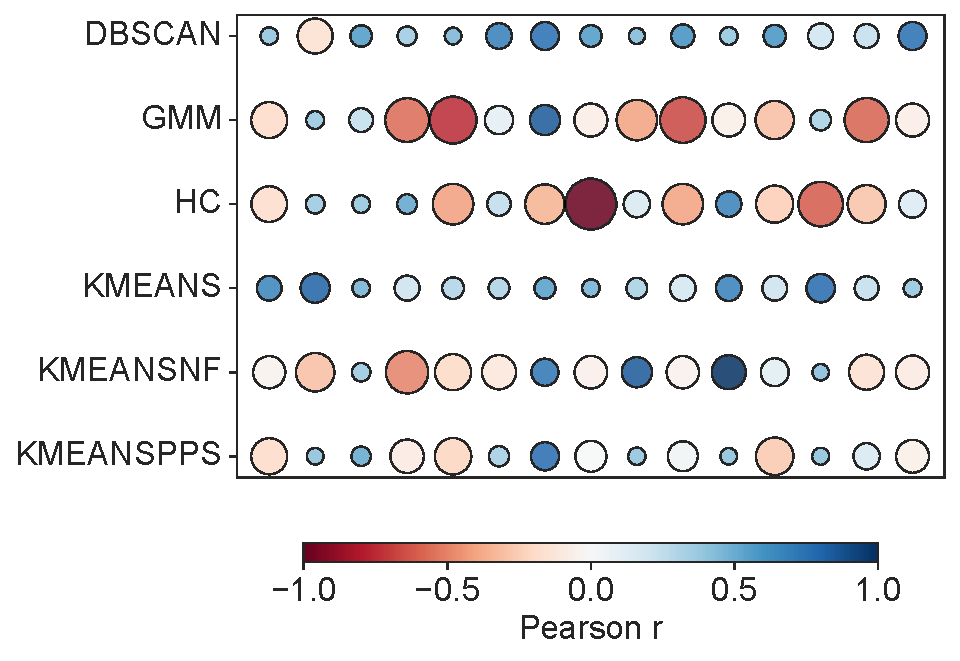
\includegraphics[width=\linewidth]{figures/6.4.3graph/BE_EDR_vs_Comb_relative.pdf}
    \caption{Beers — EDR vs.\ Comb\textsubscript{rel}}
    \label{fig:be_edr_comb}
  \end{subfigure}\hfill
  \begin{subfigure}[b]{0.33\linewidth}
    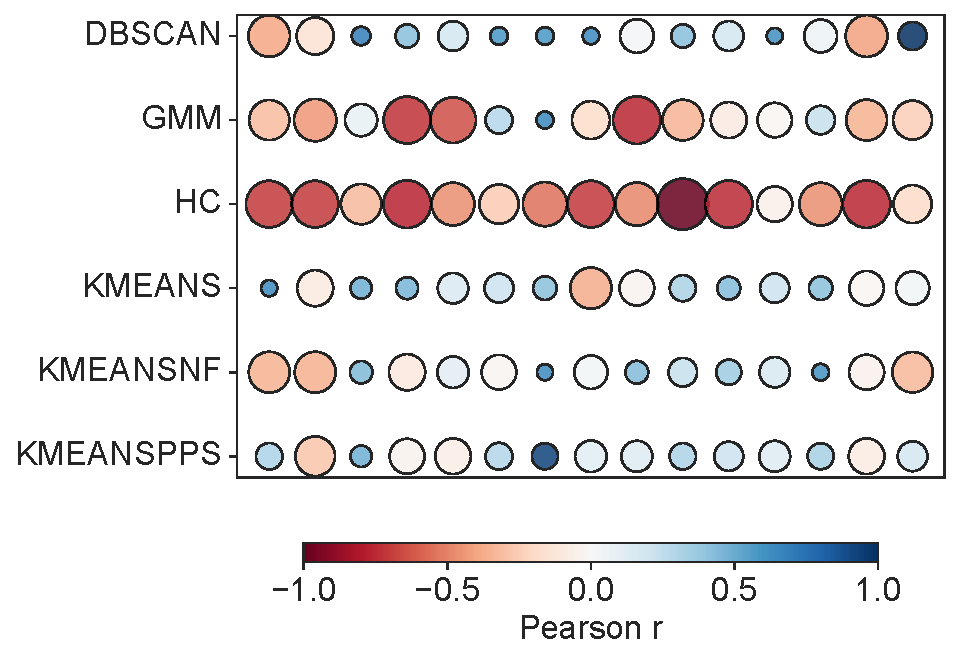
\includegraphics[width=\linewidth]{figures/6.4.3graph/BE_F1_vs_Sil_relative.pdf}
    \caption{Beers — F1 vs.\ Sil\textsubscript{rel}}
    \label{fig:be_f1_sil}
  \end{subfigure}\hfill
  \begin{subfigure}[b]{0.33\linewidth}
    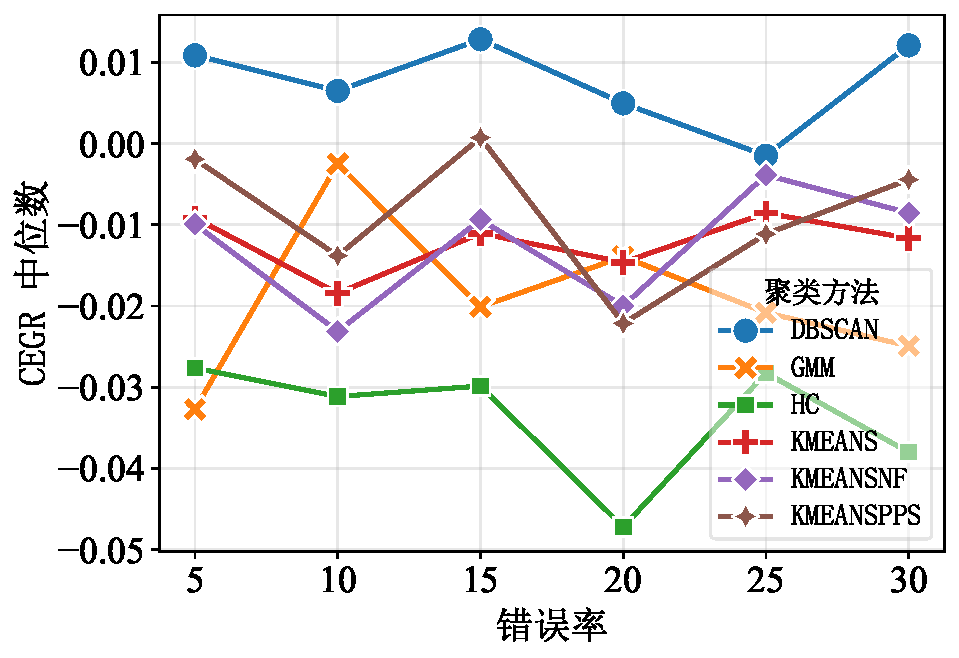
\includegraphics[width=\linewidth]{figures/6.4.3graph/CEGR_5pct_beers.pdf}
    \caption{Beers — CEGR 曲线}
    \label{fig:be_cegr}
  \end{subfigure}

  %========== 2 ─ flights ===================================================
  \begin{subfigure}[b]{0.33\linewidth}
    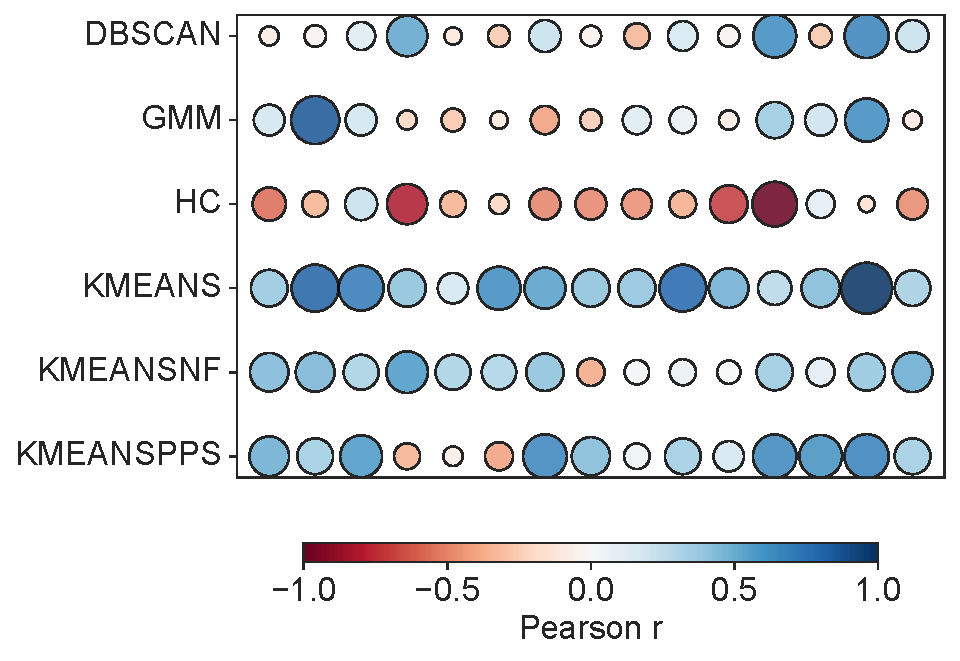
\includegraphics[width=\linewidth]{figures/6.4.3graph/FL_EDR_vs_Comb_relative.pdf}
    \caption{Flights — EDR vs.\ Comb\textsubscript{rel}}
    \label{fig:fl_edr_comb}
  \end{subfigure}\hfill
  \begin{subfigure}[b]{0.33\linewidth}
    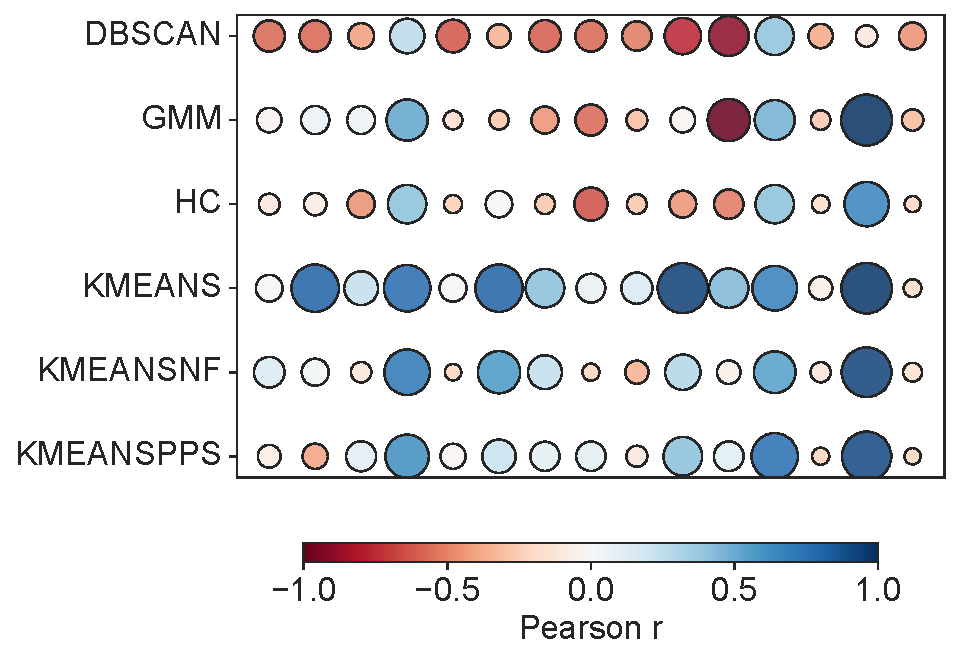
\includegraphics[width=\linewidth]{figures/6.4.3graph/FL_F1_vs_Sil_relative.pdf}
    \caption{Flights — F1 vs.\ Sil\textsubscript{rel}}
    \label{fig:fl_f1_sil}
  \end{subfigure}\hfill
  \begin{subfigure}[b]{0.33\linewidth}
    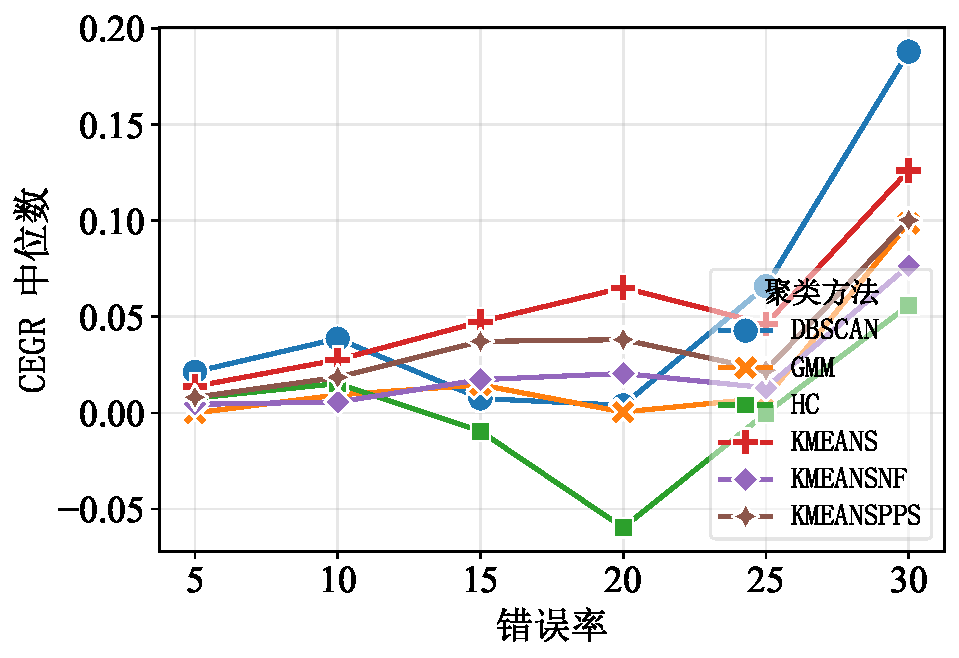
\includegraphics[width=\linewidth]{figures/6.4.3graph/CEGR_5pct_flights.pdf}
    \caption{Flights — CEGR 曲线}
    \label{fig:fl_cegr}
  \end{subfigure}

  %========== 3 ─ hospital ==================================================
  \begin{subfigure}[b]{0.33\linewidth}
    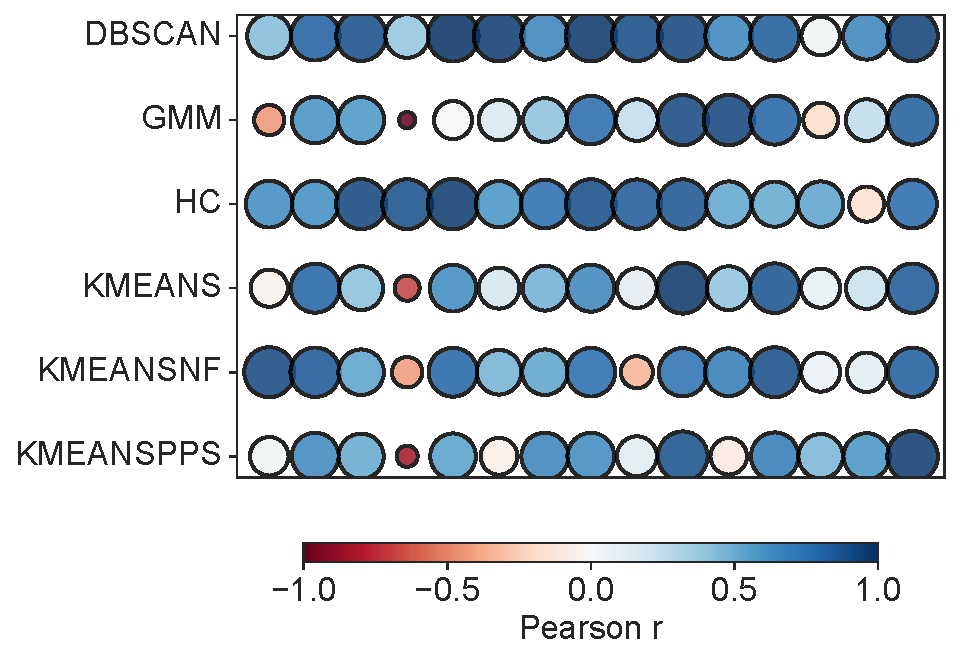
\includegraphics[width=\linewidth]{figures/6.4.3graph/HO_EDR_vs_Comb_relative.pdf}
    \caption{Hospital — EDR vs.\ Comb\textsubscript{rel}}
    \label{fig:ho_edr_comb}
  \end{subfigure}\hfill
  \begin{subfigure}[b]{0.33\linewidth}
    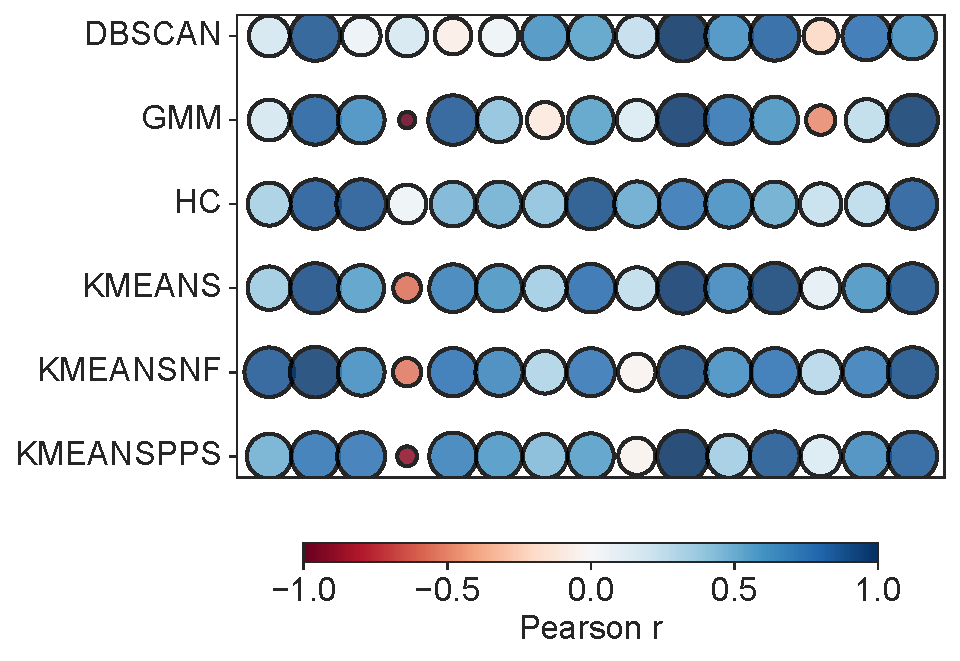
\includegraphics[width=\linewidth]{figures/6.4.3graph/HO_F1_vs_Sil_relative.pdf}
    \caption{Hospital — F1 vs.\ Sil\textsubscript{rel}}
    \label{fig:ho_f1_sil}
  \end{subfigure}\hfill
  \begin{subfigure}[b]{0.33\linewidth}
    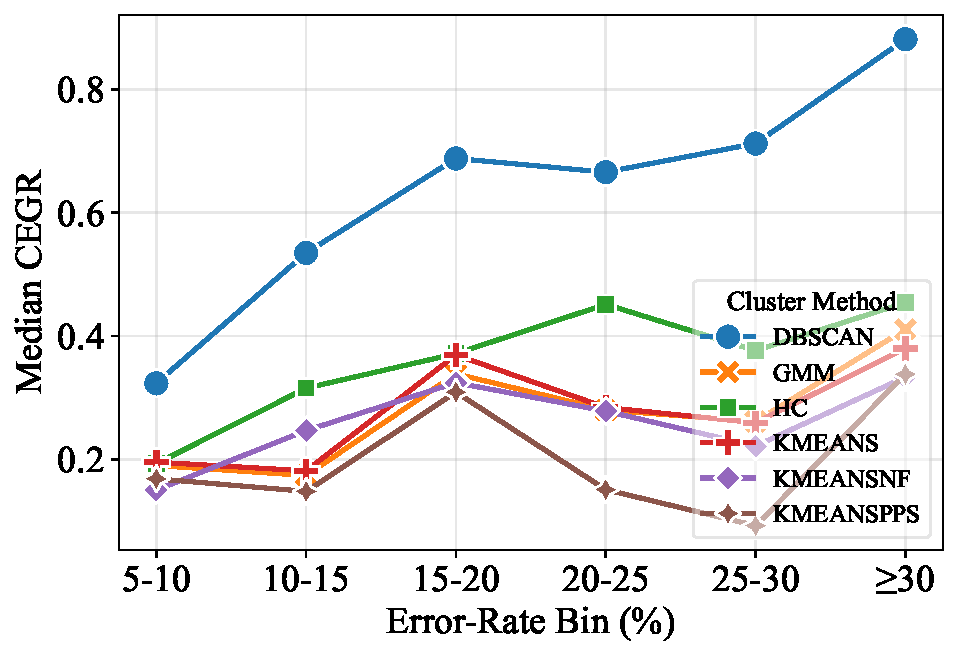
\includegraphics[width=\linewidth]{figures/6.4.3graph/CEGR_5pct_hospital.pdf}
    \caption{Hospital — CEGR 曲线}
    \label{fig:ho_cegr}
  \end{subfigure}

  %========== 4 ─ rayyan ====================================================
  \begin{subfigure}[b]{0.33\linewidth}
    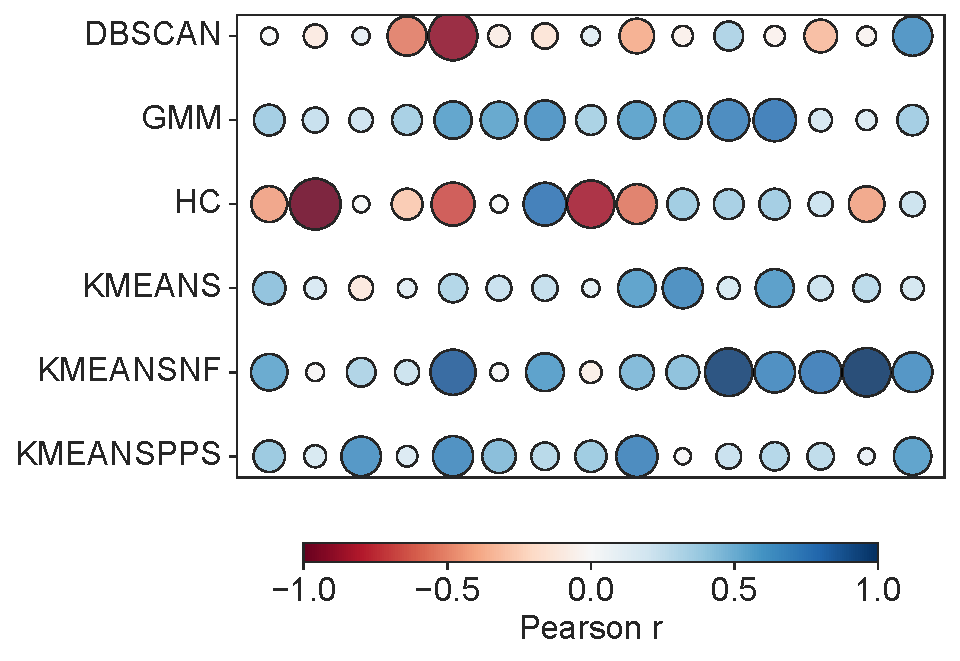
\includegraphics[width=\linewidth]{figures/6.4.3graph/RA_EDR_vs_Comb_relative.pdf}
    \caption{Rayyan — EDR vs.\ Comb\textsubscript{rel}}
    \label{fig:ra_edr_comb}
  \end{subfigure}\hfill
  \begin{subfigure}[b]{0.33\linewidth}
    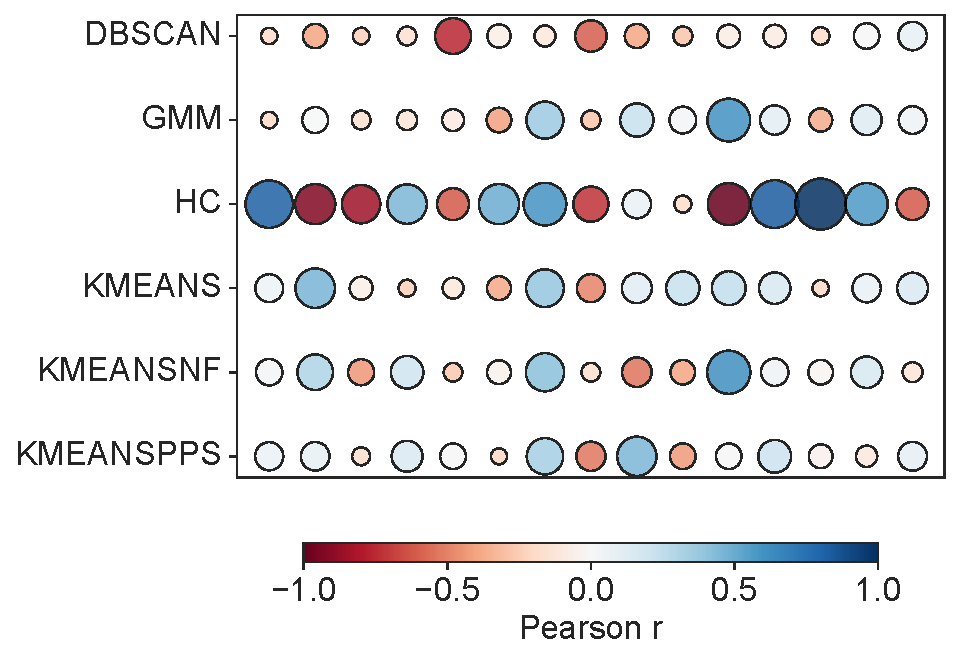
\includegraphics[width=\linewidth]{figures/6.4.3graph/RA_F1_vs_Sil_relative.pdf}
    \caption{Rayyan — F1 vs.\ Sil\textsubscript{rel}}
    \label{fig:ra_f1_sil}
  \end{subfigure}\hfill
  \begin{subfigure}[b]{0.33\linewidth}
    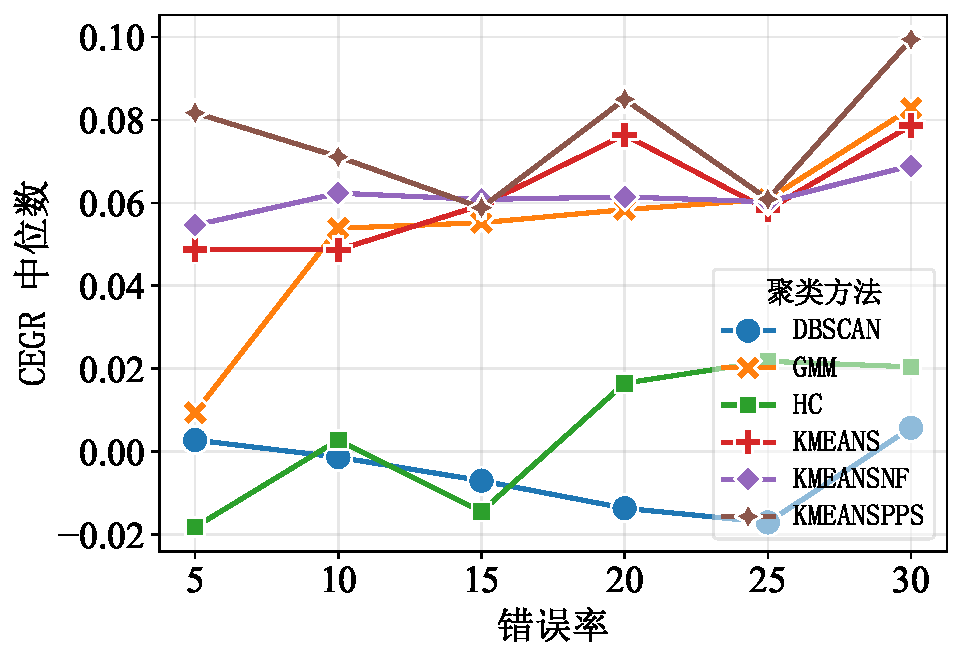
\includegraphics[width=\linewidth]{figures/6.4.3graph/CEGR_5pct_rayyan.pdf}
    \caption{Rayyan — CEGR 曲线}
    \label{fig:ra_cegr}
  \end{subfigure}

  \caption{四个数据集的“清洗–聚类”相关性与收益趋势:  
           每行同一数据集——左、中的散点图展示 Pearson 相关性;右侧折线图给出随错误率递增的 CEGR 中位数。}
  \label{fig:scatter_line_grid}
\end{figure}


% =======================================================================
\subsection{超参数选择偏移}
\label{subsec:param_shift}

在前面三节(§6.1–§6.3)中,我们已经依次阐明了
(i)不同错误分布对聚类结构的直接扰动,
(ii)各清洗策略对过程指标(质心收敛、邻域密度等)的调节效应,
以及(iii)清洗-聚类组合对最终簇质量的增益或折损。
本节旨在进一步回答一个顺理成章却尚未量化的问题:  
\textcolor[rgb]{0.00,0.07,1.00}{当数据质量与清洗策略发生变化时,聚类算法的最优超参数会否出现系统性的“漂移”,
且这种漂移是否显著到需要在 AutoML 中动态调整搜索空间?}

为进一步量化数据质量与清洗策略对聚类调参的影响,本节将建立以下两张表格:表~\ref{tab:hyper-drift} 汇总不同错误率区间下各清洗方法对 $k$、$\varepsilon$ 与协方差类型的偏移方向与幅度,给出超参数“收缩/放宽”最突出的策略及其噪声阈点;表~\ref{tab:anova} 则报告 “错误率 × 清洗方法” 两因素 ANOVA 的主效应与交互效应显著性(R\textsuperscript{2}, $F$, $p$),判定何时必须保留宽搜索窗、何时可安全剪枝。深入分析两张表格,我们可以得到以下三条主要结论:

% siunitx 设置
\sisetup{
  round-mode            = places,
  round-precision       = 3,
  detect-weight         = true,
  table-align-text-post = false
}

% 自定义显著性符号
\newcommand{\sigfilled}{\ding{72}}   % 实心五角星
\newcommand{\sighollow}{\ding{73}}   % 空心五角星

%────────────────── 表 10:超参数漂移 ──────────────────%
\begin{table*}[t]
\caption{各错误率档位下最优超参数相对基准的中位漂移(负值=收缩;正值=放宽)}
  \centering\footnotesize
  %=========== 子表 (a) Δk ===========%
  \begin{subtable}[t]{\textwidth}
    \centering
    \caption{聚类簇数漂移$\boldsymbol{\Delta k}$}  % (a) 会自动添加
    \resizebox{\textwidth}{!}{%
      \begin{tabular}{lccccccccc}
        \toprule
        \textbf{错误档位 (\%)} &
          GroundTruth & Unified & Baran & Bigdansing & BoostClean &
          HoloClean & Horizon & Mode & Scared \\
        \midrule
        0--5   & 0 & -7  & -0.5 &  0.5 & -8  & -5.5 & -3   & -2.5 & -10  \\
        5--10  & 0 & -3  &  0   &  0   & -9  & -0.5 & -5   &  4   & -8   \\
        10--15 & 0 & -11 & -4   & -6.5 & -11 & -4   & -8   & -1.5 & -13.5\\
        15--25 & 0 & -11 & -0.5 & -3.5 & -12 &  0   & -5   &  1   & -5   \\
        25--30 & 0 & -6  & -3   & -2.5 & -12 &  2   & -4.5 &  5   & -5   \\
        $\ge$30 & 0 & -4 & -3.5 & -1   & -11.5 & 2.5 & -4 & 12 & -4 \\
        \bottomrule
      \end{tabular}}
  \end{subtable}

  \bigskip

  %=========== 子表 (b) Δε ===========%
  \begin{subtable}[t]{\textwidth}
    \centering
    \caption{密度阈值漂移$\boldsymbol{\Delta\varepsilon}$}  % (b) 自动添加
    \resizebox{\textwidth}{!}{%
      \begin{tabular}{lccccccccc}
        \toprule
        \textbf{错误档位 (\%)} &
          GroundTruth & Unified & Baran & Bigdansing & BoostClean &
          HoloClean & Horizon & Mode & Scared \\
        \midrule
        0--5   & 0 &  0.065 &  0.155 & -0.735 &  0.060 & -0.175 & -0.445 & -0.455 & -0.380 \\
        5--10  & 0 &  0.060 &  0.040 & -0.050 &  0.080 & -0.060 &  0.050 & -0.090 & -0.010 \\
        10--15 & 0 &  0.020 &  0     &   0    &   0    & -0.155 &   0    & -0.035 &  0.010 \\
        15--25 & 0 &  0.010 &  0     &   0    &   0    & -0.040 &  0.020 & -0.030 &  0.020 \\
        25--30 & 0 & -0.070 & -0.010 & -0.110 & -0.050 & -0.020 & -0.135 & -0.555 & -0.040 \\
        $\ge$30 & 0 & -0.035 &  0.105 & -0.480 & -0.615 &  0.105 &  0.030 &  0.085 & -0.175 \\
        \bottomrule
      \end{tabular}}
  \end{subtable}

  %=========== 主表 caption ===========%
  \label{tab:hyper-drift}
\end{table*}


%----------- 修订后的 Table 11 --------------------------------%
\begin{table}[t]
\caption{Error-Rate × Cleaning 二因素 ANOVA 结果($n=432$)。  
           显著性:\sigfilled\,$p<0.05$,\sighollow\,$p<0.01$,\dag\,$p<0.001$.}
  \centering\footnotesize
  \begin{tabular}{
      l
      S[table-format=1.3]  % R²
      S[table-format=2.3]  % F
      c                    % p (改成普通文本列)
      S[table-format=1.3]
      S[table-format=2.3]
      c
      S[table-format=1.3]
      S[table-format=1.3]
      c}
    \toprule
            & \multicolumn{3}{c}{\textbf{错误率主效应}}
            & \multicolumn{3}{c}{\textbf{清洗主效应}}
            & \multicolumn{3}{c}{\textbf{交互效应}} \\
    \cmidrule(lr){2-4}\cmidrule(lr){5-7}\cmidrule(l){8-10}
    \textbf{参数} &
      {$R^{2}$} & {$F$} & {$p$} &
      {$R^{2}$} & {$F$} & {$p$} &
      {$R^{2}$} & {$F$} & {$p$} \\
    \midrule
    $\Delta k$ &
      0.031 & 15.044 & $<\num{1.6e-14}$\textsuperscript{\dag} &
      0.108 & 32.729 & $<\num{9.0e-49}$\textsuperscript{\dag} &
      0.025 &  1.532 & 0.018\textsuperscript{\sigfilled} \\
    $\Delta\varepsilon$ &
      0.038 &  4.417 & 0.001\textsuperscript{\dag}      &
      0.068 &  4.948 & $<\num{6.8e-06}$\textsuperscript{\dag} &
      0.084 &  1.221 & 0.172 \\
    $\Delta\text{cov}$ &
      0.006 &  3.775 & 0.002\textsuperscript{\sighollow} &
      0.008 &  2.951 & 0.003\textsuperscript{\sighollow} &
      0.007 &  0.532 & 0.993 \\
    \bottomrule
  \end{tabular}
  \label{tab:anova}
\end{table}


\medskip
\noindent%
\textbf{聚类簇数 \(k\) 的“收缩效应”随噪声强度线性放大,且由清洗策略主导.}\;

表\ref{tab:hyper-drift} 显示,在全部错误率档位中,\textit{Unified} 与 \textit{boostclean} 的 \(\Delta k\) 均保持显著负偏移(最大 \(-13.5\)),而 \textit{horizon} 与 \textit{mode} 在 \(\ge 30\%\) 档出现正偏移(+12、+5),形成明显的“收缩—扩张”对照。两因素 ANOVA 进一步印证:清洗方法主效应解释度最高(\(R^{2}=0.108,\;F=32.7,\;\dagger p<0.001\)),其次为错误率(\(R^{2}=0.031,\;F=15.0,\;\dagger p<0.001\)),交互项虽显著(\(\star p\approx0.018\))但解释度仅 \(2.5\%\)。结合 §6.2 的发现,可得:\textcolor[rgb]{0.00,0.07,1.00}{\(k\) 的最优值主要由清洗方法决定,噪声水平仅作线性拉伸;因此在 AutoML 中可按清洗法设定窄窗(\(\pm2\))并随错误率作线性修正。 }

\medskip
\noindent%
\textbf{密度阈值 \(\varepsilon\) 的漂移幅度有限,主要受单因素驱动,交互作用可忽略.}\; 

\(\Delta\varepsilon\) 的绝对值整体落在 \(\pm0.8\) 区间,仅在 0–5\,\% 档对大部分方法出现 0.06–0.16 的轻微正漂移;中高噪声时多为微负或趋零。ANOVA 结果给出:错误率与清洗方法均显著(\(\dagger p<0.001\)),但解释度分别仅 \(3.8\%\) 与 \(6.8\%\);交互项不显著(\(p\approx0.17\))。\textcolor[rgb]{0.00,0.07,1.00}{这说明\(\varepsilon\) 的最优调整更多取决于单一因素,而“噪声\(\times\)清洗”的协同效应可忽略。依据 §6.4.1 结果,可将  \(\varepsilon\) 搜索窗统一收窄至 \(\pm10\%\),并在高噪声(\(>25\%\))情形下允许一次性右移约 0.05。  }

\medskip
\noindent%
\textbf{协方差类型几乎不受数据质量与清洗策略影响,可视为稳态超参数.}\;

所有组合中 \(\Delta\text{cov}\) 恒为 0(未发生类型变更),ANOVA 各效应 \(R^{2}\) 均不足 \(0.8\%\),虽主效应达到显著(\(\star p<0.01\)),但解释度极小且交互完全不显著(\(p\approx0.99\))。结合 §6.3 已证实“协方差形态对综合评分影响边际化”,我们得出:\textcolor[rgb]{0.00,0.07,1.00}{covariance type 可固定为基准设置(如 \texttt{tied}),无须在 AutoML 搜索空间中保留可调维度,可直接削减约 12–15\,\% 的评估开销而无显著性能风险。 }

\subsection{原理驱动的 \textit{AutoML} 改进与搜索经验}
\label{sec:6.5}

回顾第6.1到第6.4节的多角度系统剖析,我们可以把清洗–聚类闭环中得到的规律归并为三条互补的\textit{AutoML} 优化路径:\emph{特征增强、阈值裁剪、动态调优}。它们既在离线阶段缩窄候选空间,又在在线阶段提升了收敛效率与最终质量,并为结果解释留下可追踪的过程信号,具体如下。

\begin{enumerate}[leftmargin=1.6em,itemsep=4pt]
  \item \textbf{错误机理特征化}  \\
        通过引入\textbf{净修复量}~(EDR)、\textbf{错误类型分布}~($r_{\mathrm{miss}}, r_{\mathrm{anom}}$) 及\textbf{过程级指标}(如~$\rho_{\text{noise}}$, $\Delta n_{\text{merge}}$, GeoDecay),
        将原特征向量 $x(D)$ 扩展为 $\tilde{x}(D)=\langle x(D),\text{EDR},\rho_{\text{noise}},\dots\rangle$。
        相关分析($r_{ \text{EDR}\rightarrow\text{Comb}}=0.71$)证明 EDR 是解释聚类收益的首要因子,而 $\rho_{\text{noise}}$ 与 $\Delta n_{\text{merge}}$ 等过程信号则提供了错误修复在算法内部触发的具体链路,可直接作为多标签模型~$\Phi$ 的高权重特征。

  \item \textbf{阈值驱动的搜索裁剪}  \\
        大规模实验揭示了按错误分段式的收益规律:\ding{192}~$r_{\mathrm{tot}}\!<\!15\%$ 时\;EDR 与聚类得分近似线性正相关;\ding{193}~$15\%\!\le r_{\mathrm{tot}}\!<\!25\%$ 出现\emph{翻转阈},需优先削减离群而非盲目填补;\ding{194}~$r_{\mathrm{tot}}\!\ge\!25\%$ 进入\emph{饱和区},除密度法(DBSCAN) 外其余分支边际收益趋零。  
        据此,我们在 $\Omega$ 上实施两级裁剪:
        \begin{itemize}
          \item \emph{量化阈值剪枝}:若 $\hat{r}_{\mathrm{tot}}\!<\!15\%$,保留 ``清洗$+$任意聚类'';若 $15$--$25\%$,剔除高误删风险的监督导向修复与层次法;若 $\ge\!25\%$,仅保留密度族并收紧 \(\varepsilon\) 搜索界。
          \item \emph{过程信号剪枝}:实时监控 $\rho_{\text{noise}}$、$\Delta n_{\text{merge}}$;当出现 ``噪声反弹'' 或 ``树塌陷''($\Delta n_{\text{merge}}<-50\%$)时,立即回滚对应策略。
        \end{itemize}

  \item \textbf{参数漂移感知的动态调优}  \\
        清洗操作会系统性地移动最佳超参数:质心法的 $k$ 呈 $\Delta k<0$ 收缩,密度法的 \(\varepsilon\) 则有 \(\Delta\varepsilon\) < 0 的\emph{左移}趋势(平均 $-12\%$)。  
        因此,\textit{AutoML} 在第二轮微调时:
        \begin{itemize}[leftmargin=1.6em,itemsep=4pt]
          \item 以 $\widehat{\Delta \theta}$ 为中心重置局部搜索窗,避免在失效区间浪费预算;
          \item 使用\textbf{分层启发式}:先对易漂移参数($k$, \(\varepsilon\))作粗粒网格,再对稳定参数(\textit{minPts},$\;$covariance‐type)应用贝叶斯优化,两阶段均匀分配评估次数;
          \item 对高噪文本任务追加“众数$+$密度”分支并放宽 \(\varepsilon\)的上限,以防止向量冗余造成的簇碎片化。
        \end{itemize}

\end{enumerate}

\vspace{0.5em}
\noindent
\textcolor[rgb]{0.00,0.07,1.00}{综上所述,基于前序章节大量的实证与机理洞察,我们提出了一个\textbf{原理驱动、阈值自适应、过程可解释}的无监督 \textit{AutoML} 流水线。该流水线不仅在搜索效率与聚类质量之间取得权衡,更为后续在线增量更新与跨领域迁移奠定了理论与工程双重基础。}


%---------------------------------
% 第七章:结论
%---------------------------------

\section{结论}
\label{sec:conclusion}

本文提出了一种面向数据质量的自动化清洗-聚类优化方法,通过协同优化框架整合数据清洗策略与聚类算法,并利用自动化优化管线缩小搜索空间,以提升聚类效率和质量。研究的主要结论如下:

\begin{enumerate}
    \item \textbf{清洗策略与聚类算法的协同优化是提高聚类质量的关键}。  
    不同清洗-聚类组合在不同数据特征下的适配性差异显著,其中 Raha-Baran + HC 适用于高维、多特征数据,而 mode + DBSCAN 在低维数值数据上可能导致极端分割。

    \item \textbf{自动化管线有效减少搜索开销,同时保持较高聚类质量}。  
    通过多标签学习建模“数据特征—优选方案子空间”的映射,该方法在平均 5.83 倍加速的情况下,实现了聚类质量 19.20\% 的提高,部分数据集在自动化搜索下获得更优结果。

    \item \textbf{数据特征(如错误率、缺失率、噪声水平)直接影响最优策略的选择}。  
    在高错误率场景下,模式填充(mode)易导致偏差,而 Raha-Baran 在语义受限数据(如医疗、文献分析)中的适配性较优。此外,密度聚类(DBSCAN, OPTICS)对超参数敏感度较高,需要更精细的调优策略。
\end{enumerate}

\paragraph{未来工作}  
本研究为数据清洗与聚类算法的协同优化提供了理论支持和实验验证,同时为自动化机器学习在无监督场景下的应用拓展了新方向。后续研究可进一步从以下方面优化:

\begin{itemize}
    \item \textbf{数据驱动的自适应清洗策略} 
 
    结合知识图谱、深度学习等方法,提升对复杂数据缺陷(如跨属性错误)的识别与修复能力,确保输入数据的准确性和一致性,为后续聚类优化提供可靠的数据基础。

    \item \textbf{采用更精细的超参数智能调优}  

    采用贝叶斯优化、遗传算法等方法,提高聚类算法的稳定性,并增强模型的可解释性。通过智能调优,使密度聚类算法能够适应不同数据分布,减少参数选择对聚类结果的影响。

    \item \textbf{引入更先进的分类模型以优化映射}  

    为更准确地捕捉数据特征与最优清洗-聚类组合间的潜在关联,可尝试引入表达能力更强的分类模型(如深度神经网络、集成学习框架等),取代传统多标签或简单判别器。

    \item \textbf{集成最新的聚类算法和评价指标}  

    在现有框架中引入近期提出的改进型聚类算法,如自监督聚类、基于图网络的聚类方法等,以提升聚类的泛化能力。同时,结合多种最新的聚类评价指标,如稳定性度量、可解释性分析等,确保模型在不同数据集上的可靠性和适用性。
\end{itemize}

综上,本文研究表明,清洗-聚类协同优化不仅能够提升数据质量对聚类效果的影响控制能力,还能通过自动化优化方法提升搜索效率,为高噪声、大规模数据环境下的聚类任务提供了可扩展、稳健的解决方案。

%---------------------------------
% 参考文献(可选)
%---------------------------------
\begingroup
\footnotesize % 调整参考文献字体大小
\bibliographystyle{IEEEtran}
\bibliography{references}    
\endgroup

\end{document} 